  Enterprise knowledge workers have been overwhelmed by the growing
  rate of incoming data in recent years.  In this paper, we present a
  recommendation system with the goal of helping knowledge workers in
  discovering useful new content.  Specifically, our system builds
  personalized user models based on file activities on enterprise
  network file servers.  Our models use novel features that are
  derived from file metadata and user collaboration.  Through
  extensive evaluation on real world enterprise data, we demonstrate
  the effectiveness of our system with high precision and recall
  values.  Unfortunately, our experiments reveal that per-user models
  are unable to handle heavy workloads.  To address this
  limitation, we propose a novel optimization technique, Active
  Feature-based Model Selection, that predicts the user models that 
should be applied on each test file. Such a technique can reduce the 
classification time per file by as much as 23 times without sacrificing accuracy. 

  We also show how this technique can be extended to improve the
  scalability exponentially at marginal cost of prediction accuracy, e.g., we can 
 gain 169 times faster performance on average across all shares by sacrificing 4\%
  of F-score.

%% Input other tex files. Begin. %% 
\section{Introduction} 
\label{sec:introduction}
The amount of data created, replicated and consumed every year has
been growing exponentially over the
years~\cite{IDGBigDataSurvey14}.  Between 2010 and 2020, the digital
data is expected to grow by 50 times~\cite{IDCDataGrowth}.
%%
%  Since the survey was conducted last year, we cannot use below
%  sentence anymore
\comment {
The
amount of data managed by enterprises follows a similar trend and is
expected to increase by 76\% within the next 12-18 months
\cite{IDGBigDataSurvey14}.
}
%%
Following a similar trend, enterprise data was projected to
increase by 76\% within the last one and half
years~\cite{IDCDataGrowth}.  The tremendous growth of data has become one
of the biggest challenges for enterprises.  It places unreasonable
burden on enterprise users or knowledge workers.
Studies~\cite{IDGBigDataSurvey14} have shown that nearly 65\% of
knowledge workers report feeling overwhelmed by the incoming data.
The situation is further exacerbated by the fact the enterprise data
resides across heterogeneous devices and environments, including network
file servers, source control repositories, emails and file servers,
cloud applications~\cite{salesforce, office365}, and enterprise social
networks~\cite{EnterpriseSN}.  This makes finding relevant content a
very challenging task for knowledge workers.

%% Analysis of the growing data plays an
%% increasingly vital role for businesses and enterprises thus assign a
%% high priority on their ability to harness the data. At the same time,
%% the growing data places unreasonable demand on enterprise users or
%% knowledge workers to cope up with its massive volumes. Studies such as
%% \cite{IDGBigDataSurvey14} have reported that nearly 65\% of knowledge
%% workers report feeling overwhelmed by the incoming data. The situation
%% is further exacerbated by the fact that the data in enterprises is
%% stored across heterogenous devices and locations. While enterprise
%% users continue using traditional technologies such as network file
%% servers, source control repositories, emails and file servers, they
%% are also increasingly using cloud based applications
%% ~\cite{salesforce, office365} and enterprise social
%% networks~\cite{EnterpriseSN} to conduct their work. The tremendous
%% growth rate of enterprise data and the diversity in its locations make
%% finding relevant content a very challenging task for knowledge
%% workers.

In this chapter, we present a system that assists knowledge workers to
\textit{discover} relevant content by providing personalized
recommendations.  In order to serve these recommendations, our system
monitors user activity over a training period and trains per-user
access models.  Although our approach currently focuses on files on
networked file servers (shares), it could potentially be applied to other types
of data as well.  For training user models, we extract interesting
metadata features based on file path and hierarchical directory
structure.  In our experiments, we observe that many enterprise users
show a high degree of collaboration, which is inferred based on their
common file accesses.  To leverage user collaboration, we propose a
collaborative filtering aware modeling approach that provides
significant improvement over metadata-based models.  Our evaluation
uses activity logs from eight different shares of an enterprise
customer.  We measure the effectiveness of our system in providing
predictions for files that are new with respect to the training data.
Our experiments show that the metadata-based models can achieve an
average F-score of nearly 50\% at 75\% precision across all shares and users.
Our collaborative filtering-based approach remarkably improves the
same F-score to over 70\%.

Although effective, per user models are not at all efficient in terms
of the runtime performance of testing.  This is because every file
that is created or modified in a share needs to be tested against the
model of each user in the share.  This could be computationally very expensive
especially for heavy workloads with a large number of users.  For
instance, for handling a heavy workload (i.e., activity
involving high file edit rate) in our experiments, our system will
need 48 64-core machines to test all edited files.  The high computational and financial cost poses a severe
constraint that could adversely affect the adoption of our system.  To
address this issue, we propose a novel technique, called Active
Features-based Model Selection (AFMS), that automatically selects only
those user models that are highly likely to generate positive
predictions, while ignoring the models that will definitely or most likely generate
negative predictions.  Thus using this technique, a test file is
tested against only the selected models, thereby speeding up the
overall testing time.  Our experiments show that AFMS drastically
reduces testing time without any loss in the prediction accuracy.
Furthermore, we show that AFMS can be used adaptively to trade-off
marginal prediction accuracy for significant performance gains during
the periods of heavy workload.


Our previous version~\cite{dwiticeis15} of this work presented the
basic technique for modeling file accesses.  This chapter presents a
new technique, AFMS, for improving solubility, along with new
experiments and insights.  The main contributions of our work are the
following:
\begin{enumerate}
\item Propose a system to analyze user file accesses in order to train
  personalized models, and recommend relevant content with a high
  degree of accuracy
\item Propose a novel model selection technique that can speed up the
  testing time by more than 6 times on average, and by over 23 times in the best case
  without any loss in the prediction accuracy
\item Extend the model selection technique to speed up the testing time
  significantly at the cost of marginal loss in the prediction accuracy
\item Demonstrate practicality of our system using a systematic study
  and evaluation based on real world enterprise data
\end{enumerate}

%%
%%  The justification for 24 64-core machines needed
%%  What is the constriant un latency of prediction?
%%
%% In this paper we present a system that assists knowledge workers to \textit{discover} relevant content by providing personalized
%% recommendations. In order to serve the recommendations, our system
%% monitors user activity over a training period and trains per user
%% access models. We focus on files on networked file servers and use a novel tokenization approach to extract metadata based features from files that enable the training of user models. In addition to modeling user access patterns using the file metadata, we note that enterprise users demonstrate a high degree of collaboration with respect to
%% common files. Thus we also propose a collaborative filtering aware modeling approach that can leverage the user collaboration and can improve the performance of our system over that of metadata based models. 
%% We provide evaluation of the system by using activity logs from eight shares of an enterprise customer. Since the system is designed to recommend new content to users, we ensure that the test data comprises of files that are new with respect to the training data. Our experiments reveal that the metadata based models can achieve average F-score of over 90\% and average recall of over 93\% for 75\% precision. In addition, user collaboration in enterprise shares can be leveraged to get average F score of over 99\% and average recall of over 99\% for 75\% precision. 
%
%In particular, the system is designed for files on networked file servers. File servers are used by enterprises for several purposes such as storing application specific data, facilitating collaboration among users, backing up data, and hosting personal home directories. 
%
%
%
%
%In addition to improving productivity of enterprise users, the proposed system can also be used to determine which files to cache on mobile devices in scenarios of intermittent connectivity. Alternatively, it can be used to reduce network latency in cloud services by caching files on client-facing web servers or directly on clients.


%% While the evaluation demonstrates feasibility of using our system to provide recommendations with high predictive correctness, the per user modeling used in our system inhibits its scalability to large shares. Specifically, for every created or modified file in a share, the models corresponding to each user in the share need to be applied. As a result of this, the computational requirement during testing can be substantial. As an example, for a populated share experiencing high file edit rate, our system may need 24 64-core machines on average for testing. This places severe computational and financial requirements on enterprises that adopt our system to help its knowledge workers discover relevant content and may even make deploying our system infeasible for large shares. 

%Practical insights are provided relating the system performance with training duration for models, separation between training and testing and user workload.
%While existing file access prediction approaches such as \cite{yeh01-mascots,yeh01-ispass} fail to provide predictions for new files, 
%The system, however, necessiates that models are constructed for each user in a share be applied on a created or modified file. As a result, classifying a file has high computational requirement which may prevent our system from scaling to large and active shares. 

%% In order to reduce the high testing computational requirement of our system, we propose a novel Active Features based Model Selection (AFMS) approach that can \textit{select} user models that may recommend a given test file to their corresponding users. Based on this, only the selected models need to be applied on the file, thus reducing its testing time computational requirement. 
%% We show empirically and verify through experiments that AFMS can reduce the computation per file testing by more
%% than an order of magnitude without any loss in model correctness. In
%% addition, we demonstrate that AFMS can reduce the testing complexity by more than two
%% orders of magnitude with graceful degradation in model
%% correctness. Furthermore, AFMS can also enable adaptive techniques that can trade off model perdictive correctness for faster processing of files during periods of high file activity in shares. Based on the proposed approach, we show that our system can be
%% scaled up to shares accessed by large number of users and having high rates of file activity, and can be implemented using only a household machine. 

%% \cite{dwiticeis15} presents a previous version of this work. The
%% current paper presents new techniques, extensive new
%% experiments and insights as compared to \cite{dwiticeis15}. The main
%% contributions of our work are the following: 
%% \begin{enumerate}
%% \item Propose a system to analyze user file accesses to train
%%   personalized models and recommend relevant content
%% \item Propose a novel model selection approach that
%%   can reduce the high computational requirement of the system by 5 times on average and by over 20 times at maximum without any loss in predictive correctness 
%% \item Propose an approach that can lower the testing computational requirement by several orders at the cost of marginal loss in the model predictive correctness
%% \item Demonstrate viability of proposed approaches using a systematic study and evaluation based on real world enterprise data 
%% \end{enumerate}


\comment{
Rest of the paper is organized as follows.  \\ 
\textbf{pending} \\ 
\textbf{Need to draft differences with ICEIS paper too.}\\ 
}
%%%% OLD CONTENT: COMMENTING %%%
\comment{ 
Enterprise knowledge workers are inundated with new options for
conducting their work with the rise of Enterprise Social
Networks~\cite{EnterpriseSN} and cloud based
applications~\cite{salesforce, office365} alongside traditional
technologies such as email, source control repositories, network file
servers, and office software suites.  Enterprises are also embracing
new computing devices such as mobile devices and tablets in addition
to existing personal computers, laptops, workstations and servers.
The amount of enterprise data grows significantly each year: studies
estimate that unstructured data grows annually by
40-50\%~\cite{IDCDataGrowth}.  The fragmentation in the tools and
devices used to work and the sheer growth of data places increasingly
unrealistic demands on knowledge workers to keep up with the influx of
data.  In fact, it has been reported that 65\% of users have felt at
times overwhelmed by the amount of incoming
data~\cite{IDGBigDataSurvey14}.

This chapter presents a system that utilizes machine learning and
natural language processing to automate the discovery of important new
or modified content and identify which subset of users will likely use
or benefit from it. The system is designed for file servers
and is evaluated with activity collected over eight network file
servers from an enterprise customer.  Enterprises use file servers for
a myriad of purposes including storing application data, back up,
enabling collaboration, and hosting personal home directories. The
proposed system will support a wide range of applications, such as
recommender systems or server cache management systems, by providing
predictions about what data will likely be accessed in the near
future.

The system bases its predictions on user activity and content
metadata.  We track content accessed by users over a specified
training interval.  Data (i.e. access to a particular piece of
content) are represented by a set of features that include path
components (e.g., parent and ancestral directories), keywords in the
path, and extension.
% NB - if we remove tokenization details, we should remove this sentence
%We employ a novel tokenization scheme to extract salient keywords from the
%metadata because it is common to observe concatenation and uniform case in
%naming files and folders.  
Each datum represents an instance in training our model.  Combining
this training data with the files specifically accessed by the user,
this system builds personalized models to predict future file
accesses. While traditional approaches for file access prediction such
as \cite{yeh01-mascots,yeh01-ispass} cannot be applied to recommend
new files, the proposed user model based approach is generalizable
enough to be applied even to content that has not been accessed
before, or is newly created. Additionally, analysis of file activity
yields the insight that very regular patterns of collaboration occur.
The chapter demonstrates a method in which an individual's prediction
precision and recall can be greatly improved by incorporating the
predictions of all other user models.

This work makes the following contributions:
\begin{itemize}
\item Observations about the nature of enterprise file activity
\item A system that analyzes file activity and metadata and applies
  machine learning and natural language processing to provide
  predictions
%\item A method to tokenize file metadata
\item A strategy to combine the personalized models of multiple file
  users to improve the predictions of individual users
\end{itemize}
%The paper is organized as follows.  Section~\ref{sec:data} provides observations
%about file activity data. Section~\ref{sec:features} details the feature space
%and Section~\ref{sec:models} details the approach to construct and evaluate
%individual models. Section~\ref{sec:evaluation} evaluates the performance of
%this model with discussion in Section~\ref{sec:discussion}.  These sections are
%followed by related work in Section~\ref{sec:relatedwork} and a conclusion in
%Section~\ref{sec:conclusion}.

%% Redundant with first highlight - MAH
%% We evaluate the proposed approach over activity data recorded on
%%   ten network file servers activity data from an enterprise customer.  in the shares corresponds to
%%   real world data from enterprises. 

The chapter is organized as follows. 
  Section 2 provides observations about file activity and pre-processing.
  Section 3 details the feature space and
  Section 4 describes the construction of metadata and collaborative filtering-based user models.
  Section 5 presents an evaluation of the user models and 
  Section 6 discusses the contributions and characteristics of the features used
  in the models, and scalability and deployment related aspects. 
  Section 7 identifies related work followed by a discussion on directions for future work in Section 8. Section 9 concludes. 
}
%%%% OLD CONTENT: COMMENTING %%%  

\section{The File Recommendation System}
\label{sec:overallsystem}
\begin{figure}
\centering
{\fontsize{8pt}{1em}\selectfont
\begin{tabular}{c}
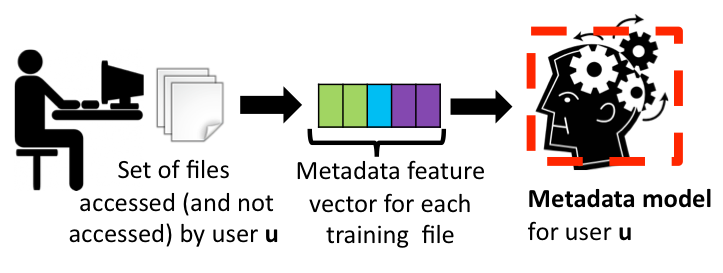
\includegraphics[trim = 0mm 0mm 0mm 4mm, clip, width=0.65\linewidth]{FileAccess/figs/meta_training} \\
\multicolumn{1}{l}{(a) \textbf{Training}: metadata models for each user} \\ 
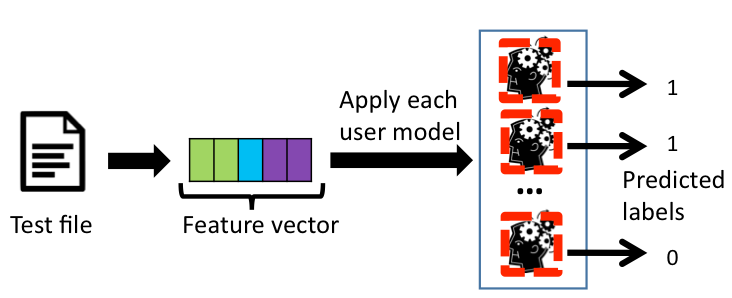
\includegraphics[trim = 0mm 0mm 0mm 7mm, clip, width=0.65\linewidth]{FileAccess/figs/testing} \\
\multicolumn{1}{l}{(b) \textbf{Testing}: apply the trained models for all users in share} \\  
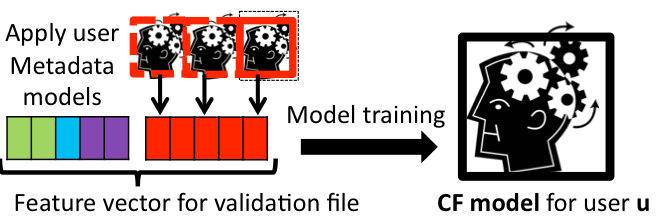
\includegraphics[width=0.62\linewidth]{FileAccess/figs/cf_training2} \\
\multicolumn{1}{l}{(c) \textbf{Training}: CF models for each user} \\  
\end{tabular}
}
\caption{Approach Overview}
\label{fig:overallfigs}
%\vspace{-0.5cm}
\end{figure}

%%
Our system uses a binary classification approach for providing file
recommendations.  For this purpose, it builds a separate
classification model for each user of a file share.  The dataset of a
given user includes all the files that have been accessed by all 
users of the share.  The label of a file in the dataset is $1$ if the
user accesses it, $0$ otherwise.  It is important to know that if a
user accesses a particular file during the training phase, it is
highly likely that the user will access the same file during the
testing phase.  Recommending such a file to the user is not very
useful.  Hence the main objective of our system is to discover useful
but new files that may have been created or modified by other users of
the same share.  For this reason, the testing phase includes only
those files that are new with respect to the training phase for the
user.  Our system then applies the model of the user to these files to
predict classification labels.  The rest of this section describes the
features and the modeling techniques used in the system.

%% The proposed system comprises of a training and a testing
%% phase. During training, file activities are monitored, features are
%% extracted from file metadata and a model per user is trained. This is shown
%% for metadata based models in Figure~\ref{fig:overallfigs}(a). During testing or classification phase (Figure~\ref{fig:overallfigs}(b)), features are
%% extracted from each created or modified file and the trained models for
%% every user in the share are applied on the file. The features used and modeling
%% techniques adopted are briefly described below.

%Details can be obtained from~\cite{dwiticeis15}. 
\subsection{Metadata Features}
\label{sec:features}
%%
The metadata features include features extracted from different
attributes of a file:
%% The metadata features of each training or test file are concatenation
%% of its folder, token and extension features.
%%
\begin{itemize}
  \renewcommand{\labelitemi}{$\bullet$}
%%
\item \textbf{Folder}:
%%
We create a folder feature corresponding to every folder and its
ancestor folders observed in the training period\footnote{Please note
  that no features are derived for completely new attributes seen only
  during the testing phase.}.  For a file $f$, we capture the folder
features as a binary vector with the value 1 in the locations
corresponding to the folder or the ancestor folders of $f$, and 0
elsewhere.  These features help in learning a user's preference for
certain subtrees of the file system hierarchy in a share without
having to define a folder distance metric.
%%
\item \textbf{Token}:
%%
We tokenize the path name of each file using a novel tokenization
approach, the details of which can be found in~\cite{dwiticeis15}.  We
construct a token vocabulary using all the tokens observed during the
training phase.  For extracting features, we capture tokens of a file
as bag-of-words representation on the entire vocabulary.
%%
\item \textbf{Extension}:
%%
We construct an extension vocabulary based on the popular extensions
observed in the training data.  We then use this vocabulary to
represent a file's extension with one-hot encoding-based features.
%%
\end{itemize}
%%
%% \begin{enumerate}
%% \item \textbf{Folder features}: We create a folder feature
%%   corresponding to every folder and its ancentor folders observed in
%%   the training period. For every training or test file $f$, its folder
%%   features are a binary vector with 1 in locations corresponding to
%%   the folder of $f$ or its ancenstors, and 0 elsewhere. This feature helps learning a user's
%% preferences for certain subtrees of the file system
%%   hierarchy in a share without the need of definining folder distance
%%   metrics.
%%
%% \item \textbf{Token features}: We tokenize the path name of each file using a novel tokenization approach, the details of which are given in ~\cite{dwiticeis15}. The tokens resulting observed during training are used to construct a token vocabulary. The tokens in each file's path are represented using bag of words representation on the constructed vocabulary. 

%% \item \textbf{Extension features}: We construct an extension vocabulary based on the popular extensions observed in the training data. One-hot encoding is
%%   used to represent the extension of each file based on the constructed extension vocabulary. 
%% \end{enumerate}
%The metadata features of a file are concatenation of its folder, token and extension features. 

\subsection{Modeling Techniques} 
\label{sec:Metamodels}
%%
We first build basic metadata models based on the metadata features.
Using these models, we then develop an innovative approach to leverage
collaboration among users for building collaborative filtering aware
models that provide better performance over the basic metadata models.
%% Our system trains per user models using the activity observed over a
%% training period. For user $u$, every file $f$ that has been read in
%% the training period is a training instance. The corresponding label is
%% 1 if $u$ has read $f$ during training, 0 otherwise. Thus while the
%% training instances for all users in a share are the same, the labels
%% may be different. For testing, every file that has been read in
%% testing period and has $not$ been seen in training is a testing
%% instance. Doing so ensures that the models are evaluated over files
%% that are new with respect to the training data. Testing labels are
%% determined in a similar manner as training labels. We approach file
%% recommendation as a classification problem and use the following
%% modeling approaches.
%Below are the two modeling aproaches used in our system. 

\subsubsection{Metadata-based Modeling}
%%
For each user, we train a metadata model using the metadata features.
Figure~\ref{fig:overallfigs} (a, b) shows the training and the testing
phases of this approach.  Considering the trade-off between accuracy
and training time efficiency~\cite{dwiticeis15}, we pick Support
Vector Machine (SVM) with a linear kernel as our modeling technique
because it provides high accuracy without incurring significant
training time.  More importantly, a linear SVM provides feature
weights that capture the relative significance of individual features.
We leverage this aspect in our scalability optimization technique AFMS
as described in Section~\ref{sec:testspeedup}.

%% For each user, we train a metadata based model using the metadata features of the training files and their labels. We have chosen Support Vector Machines (SVMs) with linear kernel as the models since they offer high accuracy without
%% incurring significant training time. \cite{dwiticeis15} provides a
%% comparison between different machine learning models. 
%% In addition, linear SVMs provide feature weights that can determine the significance of individual features, and can be leveraged for techniques such as Active Feature based Model Selection (Section~\ref{sec:testspeedup}) to improve the scalability of our system. 
%% The training and
%% testing for metadata based models is shown in
%% Figures~\ref{fig:overallfigs}(a) and \ref{fig:overallfigs}(b)
%% respectively.
\subsubsection{Collaborative Filtering (CF)-based Modeling} 
\label{sec:CFdetails}
%%
Enterprise users often show a high degree of collaboration in terms of
accessing common files in a share.  We make this observation based on
the measurement of the metric, \textit{normalized triangle count} 
(Section~\ref{sec:data}), that captures the degree of collaboration
among users.  As an illustration, see Figure~\ref{fig:snagraphs} that
shows user communities in terms of social network graphs for a couple
of shares.

We leverage user collaborations to build CF models that are
significantly more effective than the metadata models.  Here are the
details of the method used in building a CF model for a user $u$.
First, we divide the original training set into a new training set and a
validation set.  We then use the new training set to train a metadata
model for each user.  Second, for each file in the validation set, we
apply the metadata models of all the users, and generate a vector of
the resulting predicted labels.  Third, we train the CF model for the
user $u$ using the files in the validation set.  For this, we
construct the feature vector for each validation file by concatenating
the metadata features with the vector of the predicted labels
(Figure~\ref{fig:overallfigs}(c)).  For each test file observed during
the testing phase, we first apply the metadata models of all the users
to generate a vector of the predicted labels.  Finally, we append this
vector to the metadata features to create a new feature vector and
feed it to the user $u$'s CF model to obtain the final predicted
label.


An interesting point to be noted here is that our CF-based modeling
technique does not require a pre-defined user-user relationship or
even a user similarity metric.  Rather, the model can automatically learn
positive or negative correlation between the activities of users, and
accordingly adapt to make better predictions.  For instance, if two
users have similar access patterns, the CF model for one user could
learn that its labels positively correlate with labels predicted by
the other user's metadata model.  Thus, greater the degree of
collaboration, the better will be the effectiveness of the CF models.
Another benefit of our technique is that, unlike pure collaborative
filtering-based systems developed in the past, it does not suffer from
a cold-start problem.  Previous systems recommend an item to a user if
other \textit{similar} users have shown a preference for that item.
Therefore, these systems are incapable of recommending a completely
new item because no other user has seen it before.  In contrast, the
novelty of our technique is in using CF features that are based on
predicted labels rather than the history of past accesses.

%% Enterprise users demonstrate a high degree of collaboration in terms
%% of accessing common files in a share. This is validated in Section~\ref{sec:data} where we measure the collaboration among users in terms of normalized triangle counts and also demonstrate the existence of user communities in social network graphs for sample shares. For each user, we train a CF aware model that captures the
%% predictions of all metadata based user models in a share with the aim of making
%% better prediction for the user by leveraging user
%% collaboration. In order to do this, we divide the set of training files into training and validation files. The metadata based models corresponding to each user in a share are trained on the training files and each
%% metadata model is applied on each validation files, resulting
%% in a vector of predicted metadata model based labels per validation file. 
%% The CF aware model for each user is then trained using all validation files. The features used for each validation file are concatenation of its metadata features, and the vector of predicted metadata model based labels for the file. This is shown in
%% Figure~\ref{fig:overallfigs}(c). On a test file, first the metadata
%% based models of all users in a share are applied to obtain the
%% predicted metadata model based labels. They are then concatenated with the file's metadata
%% features and the CF aware models are then applied to obtain the final predicted label for the user.
%% %Such an approach enables capturing the relationships between predictions of different users in a share. 

%% The CF aware modeling as proposed above does not require a pre-defined user-user relationship or even a similarity metric. Rather, the model can automatically learn if there is positive or negative correlation between the activities of users, and accordingly adapt the model to use this information to make better predictions. For example if two users have similar access patterns, then the CF aware model for one user could learn that its labels typically correlate with labels predicted by the other user's metadata based model. It is expected that CF aware models can provide most benefit in a share that demonstrates substantial user collaboration. 
%% Another benefit of using the above approach is that unlike purely collaborative filtering based systems, the proposed approach does not suffer from cold-start problem. Systems that recommend items to a user if other \textit{similar} users have liked, accessed or purchased the item are incapable of recommending items that are completely new since there are no users who have already accessed it. As compared to these, the collaboration based features that are utilized in the CF aware models are based on \textit{predicted} labels instead of actual past accesses and are used in addition to metadata features. 


\section{Evaluation Framework}
\label{sec:evaluation}
%%
This section describes the evaluation data and methodology.
%% This section describes the data used and the experimental methodology adopted for evaluating the proposed file recommendation system. 

\subsection{Data}
\label{sec:data}
\begin{table*}[!htpb]
\centering
\caption{Statistics of shares used for evaluation } 
{\fontsize{8pt}{1em}\selectfont
%\begin{tabular}{|p{0.5cm}|p{1.28cm}|r|p{1.15cm}|p{1.1cm}|p{1.4cm}|}
  %\begin{tabular}{|>{\centering}p{0.8cm}|r|r|>{\centering}p{2.7cm}|>{\centering}p{2.3cm}|r|}
\begin{tabular}{|>{\centering}p{0.8cm}|r|r|r|r|r|}
\hline
%Share & Sample period (days) & Users & Files operated on & Total file operations &Norm. Triangle Count \\
\textbf{Share} & \textbf{\# days} & \textbf{\# users} & \textbf{\# files operated on} & \textbf{\# file operations} &\textbf{Norm. Triangle Count} \\
\hline
A & 123 & 992 & 36,009 & 11M &  8K \\ \hline
B & 122 & 464 & 1,309 & 136K &3K \\ \hline%Correction made to camera ready
C & 122 & 160 & 1,044,779 & 3M &  $<$0.1\\ \hline
D & 121 & 183 & 746 & 11K & 951\\ \hline%Correction made to camera ready
E & 66 &  1,288 & 99,733 & 292K &3K \\ \hline
F & 66 & 937 & 6,911 & 4M &0.4 \\ \hline
G & 66 & 198 & 334 & 14K  & 3K \\ \hline
H & 57 & 398 & 133,006 & 4M  &45\\  \hline
\end{tabular}
\label{tab:datasetstats1}
}
\end{table*}

%%
\begin{figure*}[!htbp]
\centering
\begin{tabular}{cc}
\centering
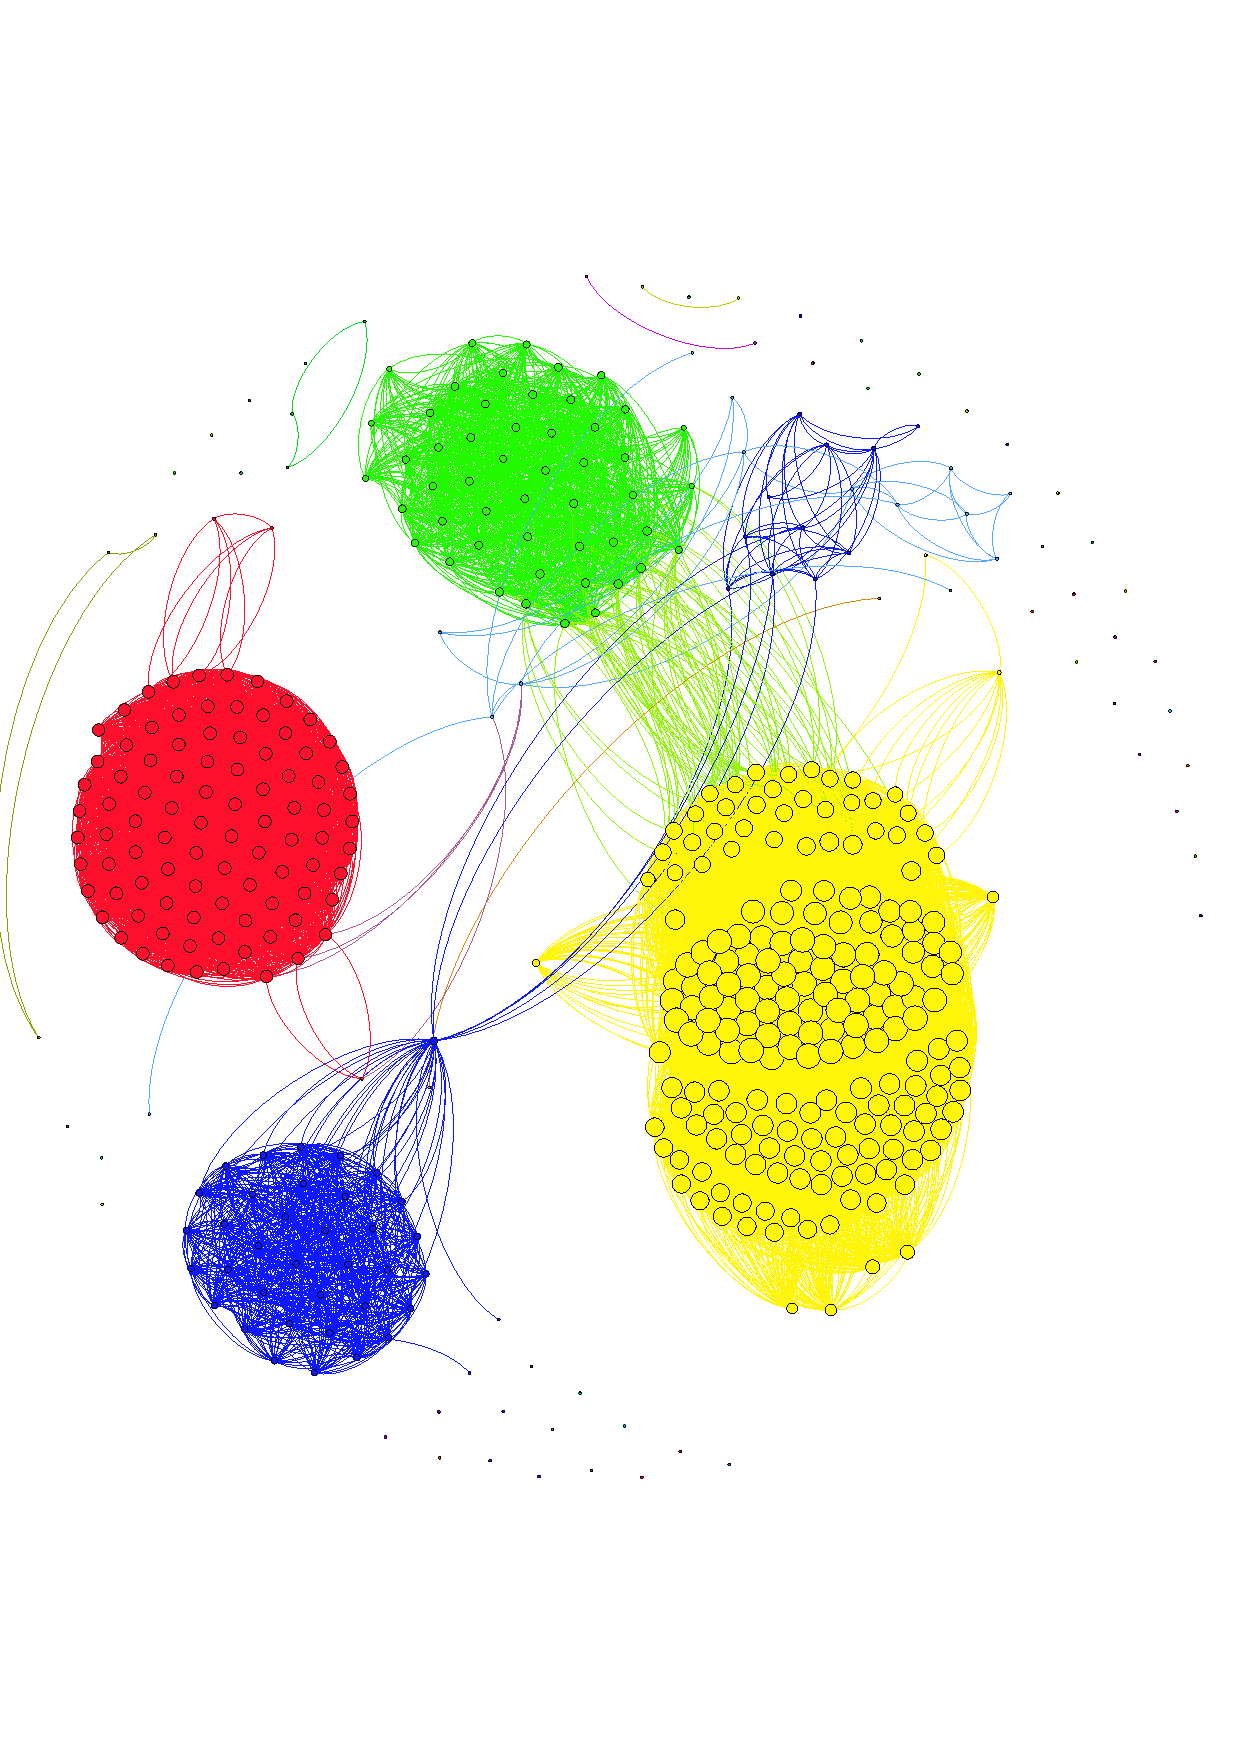
\includegraphics[trim = 0 4cm 2mm 5cm, clip, width=0.45\linewidth]{FileAccess/figs/6261_jacc_pt5}
& 
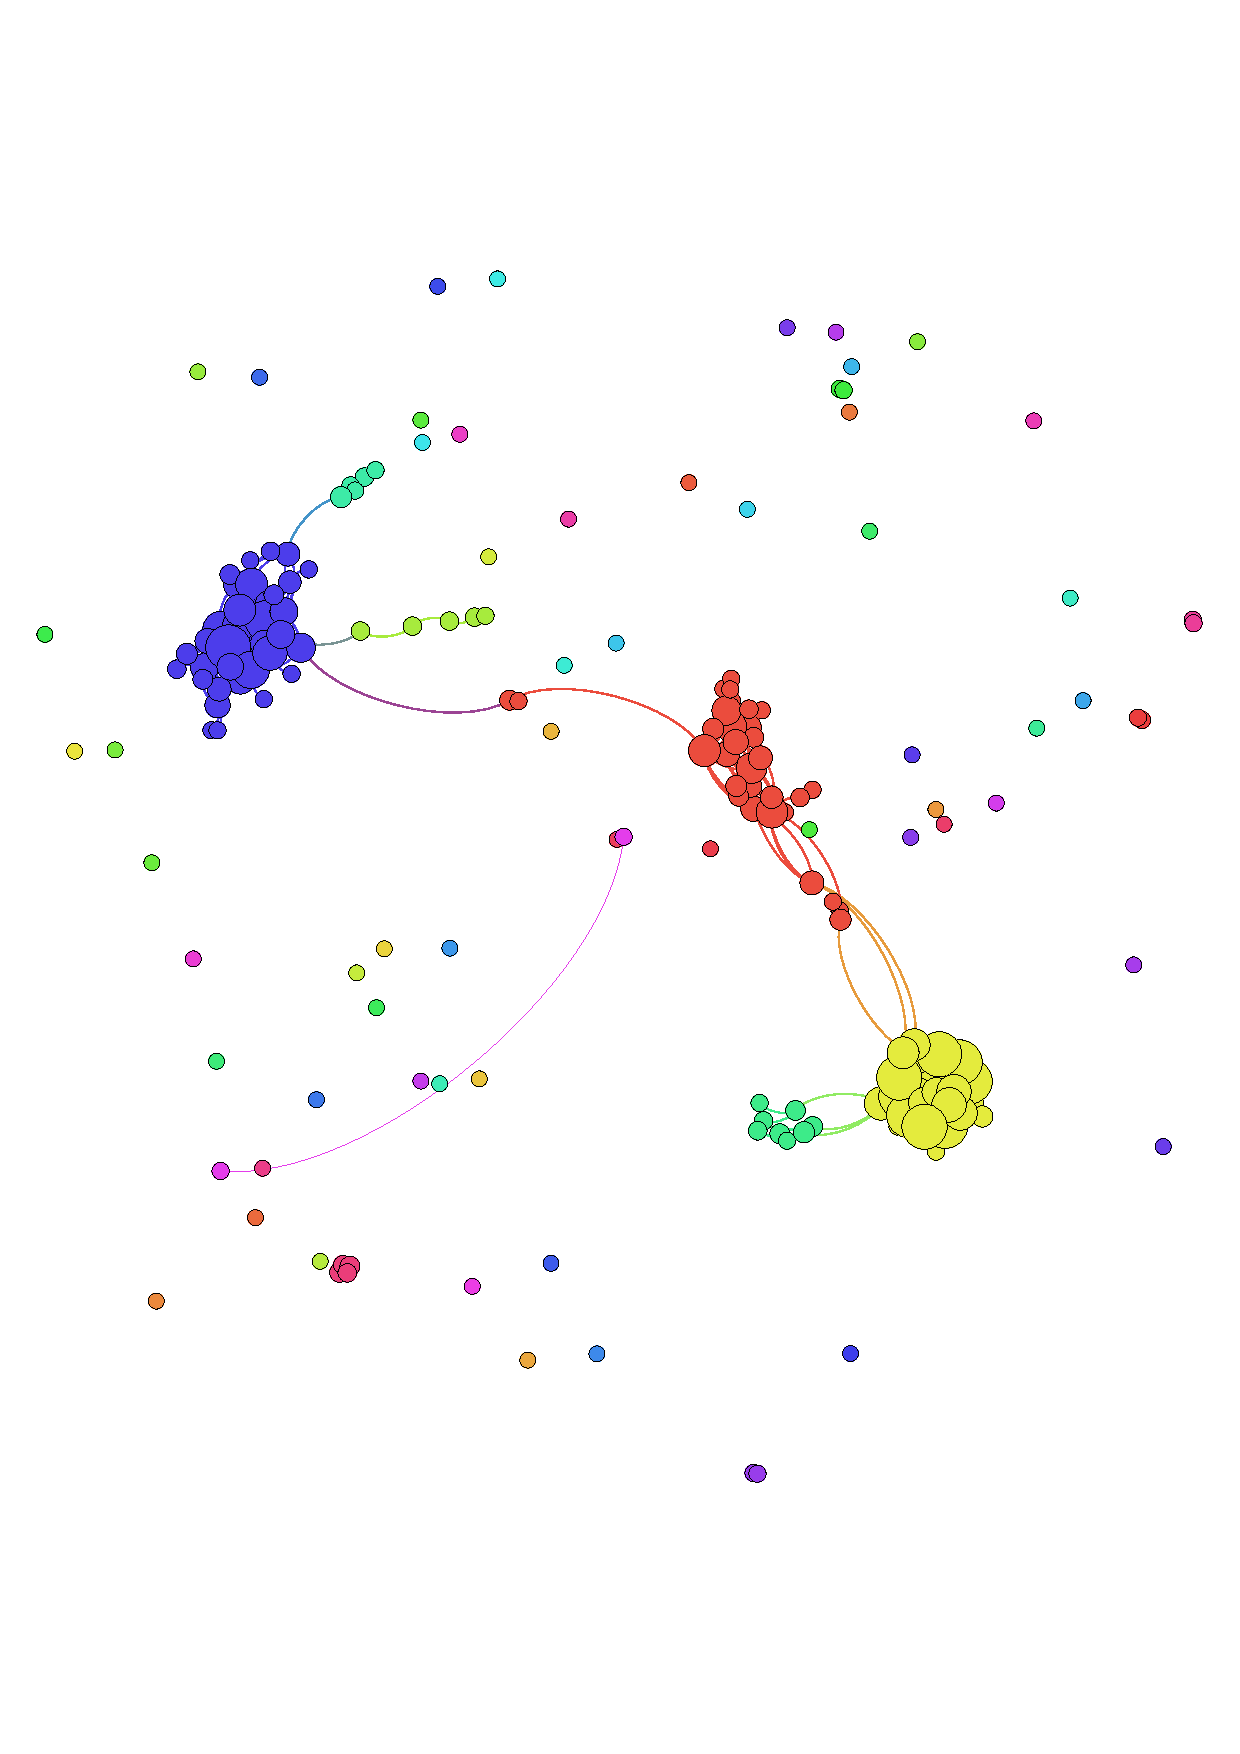
\includegraphics[trim = 2mm 4cm 7mm 5cm, clip, width=0.46\linewidth]{FileAccess/figs/6216_jacc_pt5} \\ 
(a) Share B & (b) Share D \\ 
\end{tabular}
%%
\caption[Social network graphs for shares show that users collaborate
  and tend to form communities by accessing common files. ]{Social network graphs for shares show that users collaborate
  and tend to form communities by accessing common files.  In these
  graphs, each node corresponds to a user, and an edge connects two users
  when the Jaccard index of common files accessed by those users is
  above $0.5$.}
%%
\label{fig:snagraphs}
\end{figure*}
We use file activity logs from eight network file shares of an
enterprise customer for evaluation.  Table~\ref{tab:datasetstats1}
provides key statistics of this data.  Because our recommendation
system targets user collaborations, we select shares from
90\textsuperscript{th} percentile in terms of triangle count -- a
metric to capture degree of collaboration among users.  Triangle count
for a share is the number of triangles formed, where a triangle edge
corresponds to a connection between two users based on accessing at
least one common file.  The table shows the triangle count values
normalized with respect the number of files.  For better
visualization, see Figure~\ref{fig:snagraphs} that shows users forming
different communities based on their collaborations. \\

%% We use the activity log data from eight network file servers (shares) of an enterprise customer for evaluation.
%% %The reader is directed to \cite{dwiticeis15} for details on workload statistics and popular files in these shares. 
%% The selected shares fall in the 90\textsuperscript{th} percentile in
%% terms of total number of triangle counts, i.e., number of triangles
%% formed when two users are connected if there exists at least one file
%% that both users have accessed. Table~\ref{tab:datasetstats1} captures
%% their key statistics. We measure the collaboration among users in a share based on the triangle counts normalized with respect to the number
%% of files. Figures~\ref{fig:snagraphs}(a) and (b) show the social
%% network graphs for users in two shares. It can be seen that the users tend to
%% form communities by co-accessing files.

\noindent\textbf{Removal of automated activity}: 
\label{sec:removebursts}
%%
We observe two types of file activities in our data.  The first
corresponds to the activities that are manually initiated by
users. These activities are characterized by a low number of file
operations per hour.  The second corresponds to scripted activities
that are performed by automated computer programs or scripts.  These
activities are generally seen as bursts or exceptionally high number
of file operations per hour.  Since our goal is to assist knowledge
workers and not automated programs, we need to remove the scripted
activity from the evaluation data.  For this purpose, we remove
the activities by a user in an hours if the number of activities are 
determined to be exceptionally high. Towards this, an appropriate threshold 
is determined using Tukey's outlier
factor~\cite{wang2011statistical}.\linebreak

%% We note from our data that user file activities typically constitute of two modes of operation. The first corresponds to users deliberately performing an action in the file system and is characterized by low number of file operations per hour. The second mode corresponds to scripted activity performed by computer programs or scripts and is seen as bursts or exceptionally high number of file operations per hour. Since our system is designed to assist knowledge workers and not automated computer programs operating from their accounts, the scripted activity should be removed from the evaluation data. We approach this as an anomaly detection problem and argue that if a user is seen to make a high number of file operations per hours, then a large fraction of the actions were scripted. We use Tukey's outlier factor~\cite{wang2011statistical} to determine an appropriate threshold on the number of activities per user per hour. The activity by a user in an hour is labeled scripted and removed if the number of file operations by the user in the hour are above the calculated threshold. 
%% %In order to avoid discarding actual user activity, the threshold is empirically set to 1000 which is above the threshold calculated using~\cite{wang2011statistical}. If a user is seen as making more than 1000 file operations per hour, then a large fractions of the actions were scripted. 
%% The data obtained after removal of scripted activity is used for the rest of the paper. 

\noindent\textbf{Selection of evaluation users}: 
\label{sec:selectusers} 
%
Since our system helps users discover new or modified content, it is
primarily targeted for active users.  Therefore, for each share, we
sample 30 users from the highest quartile of users in terms of number
of activities, and use them in our evaluation.
%% Since our system helps users discover new or modified content, it is most useful for active users. Thus for each evaluation share, we sample 30 users from the highest quartile of users in terms of number of activities, and use them to evaluate our system. 
%
\subsection{Evaluation Methodology}
\label{evalmethodology}
%%
We experiment with different training and testing periods to evaluate the
performance of our system under different settings. 

%%
%Per user models are trained over the training period and tested on actual user activities in the testing period. Experiments are conducted by varying the training and testing periods as described below. 

%% We experiment with different training and testing periods to study the performance of our system under different settings. 
%% %Per user models are trained over the training period and tested on actual user activities in the testing period. Experiments are conducted by varying the training and testing periods as described below. 

\subsubsection{Varying training and test periods} 
\label{sec:varytraintest} 
\begin{figure}[!htbp]
\begin{center}
\centering
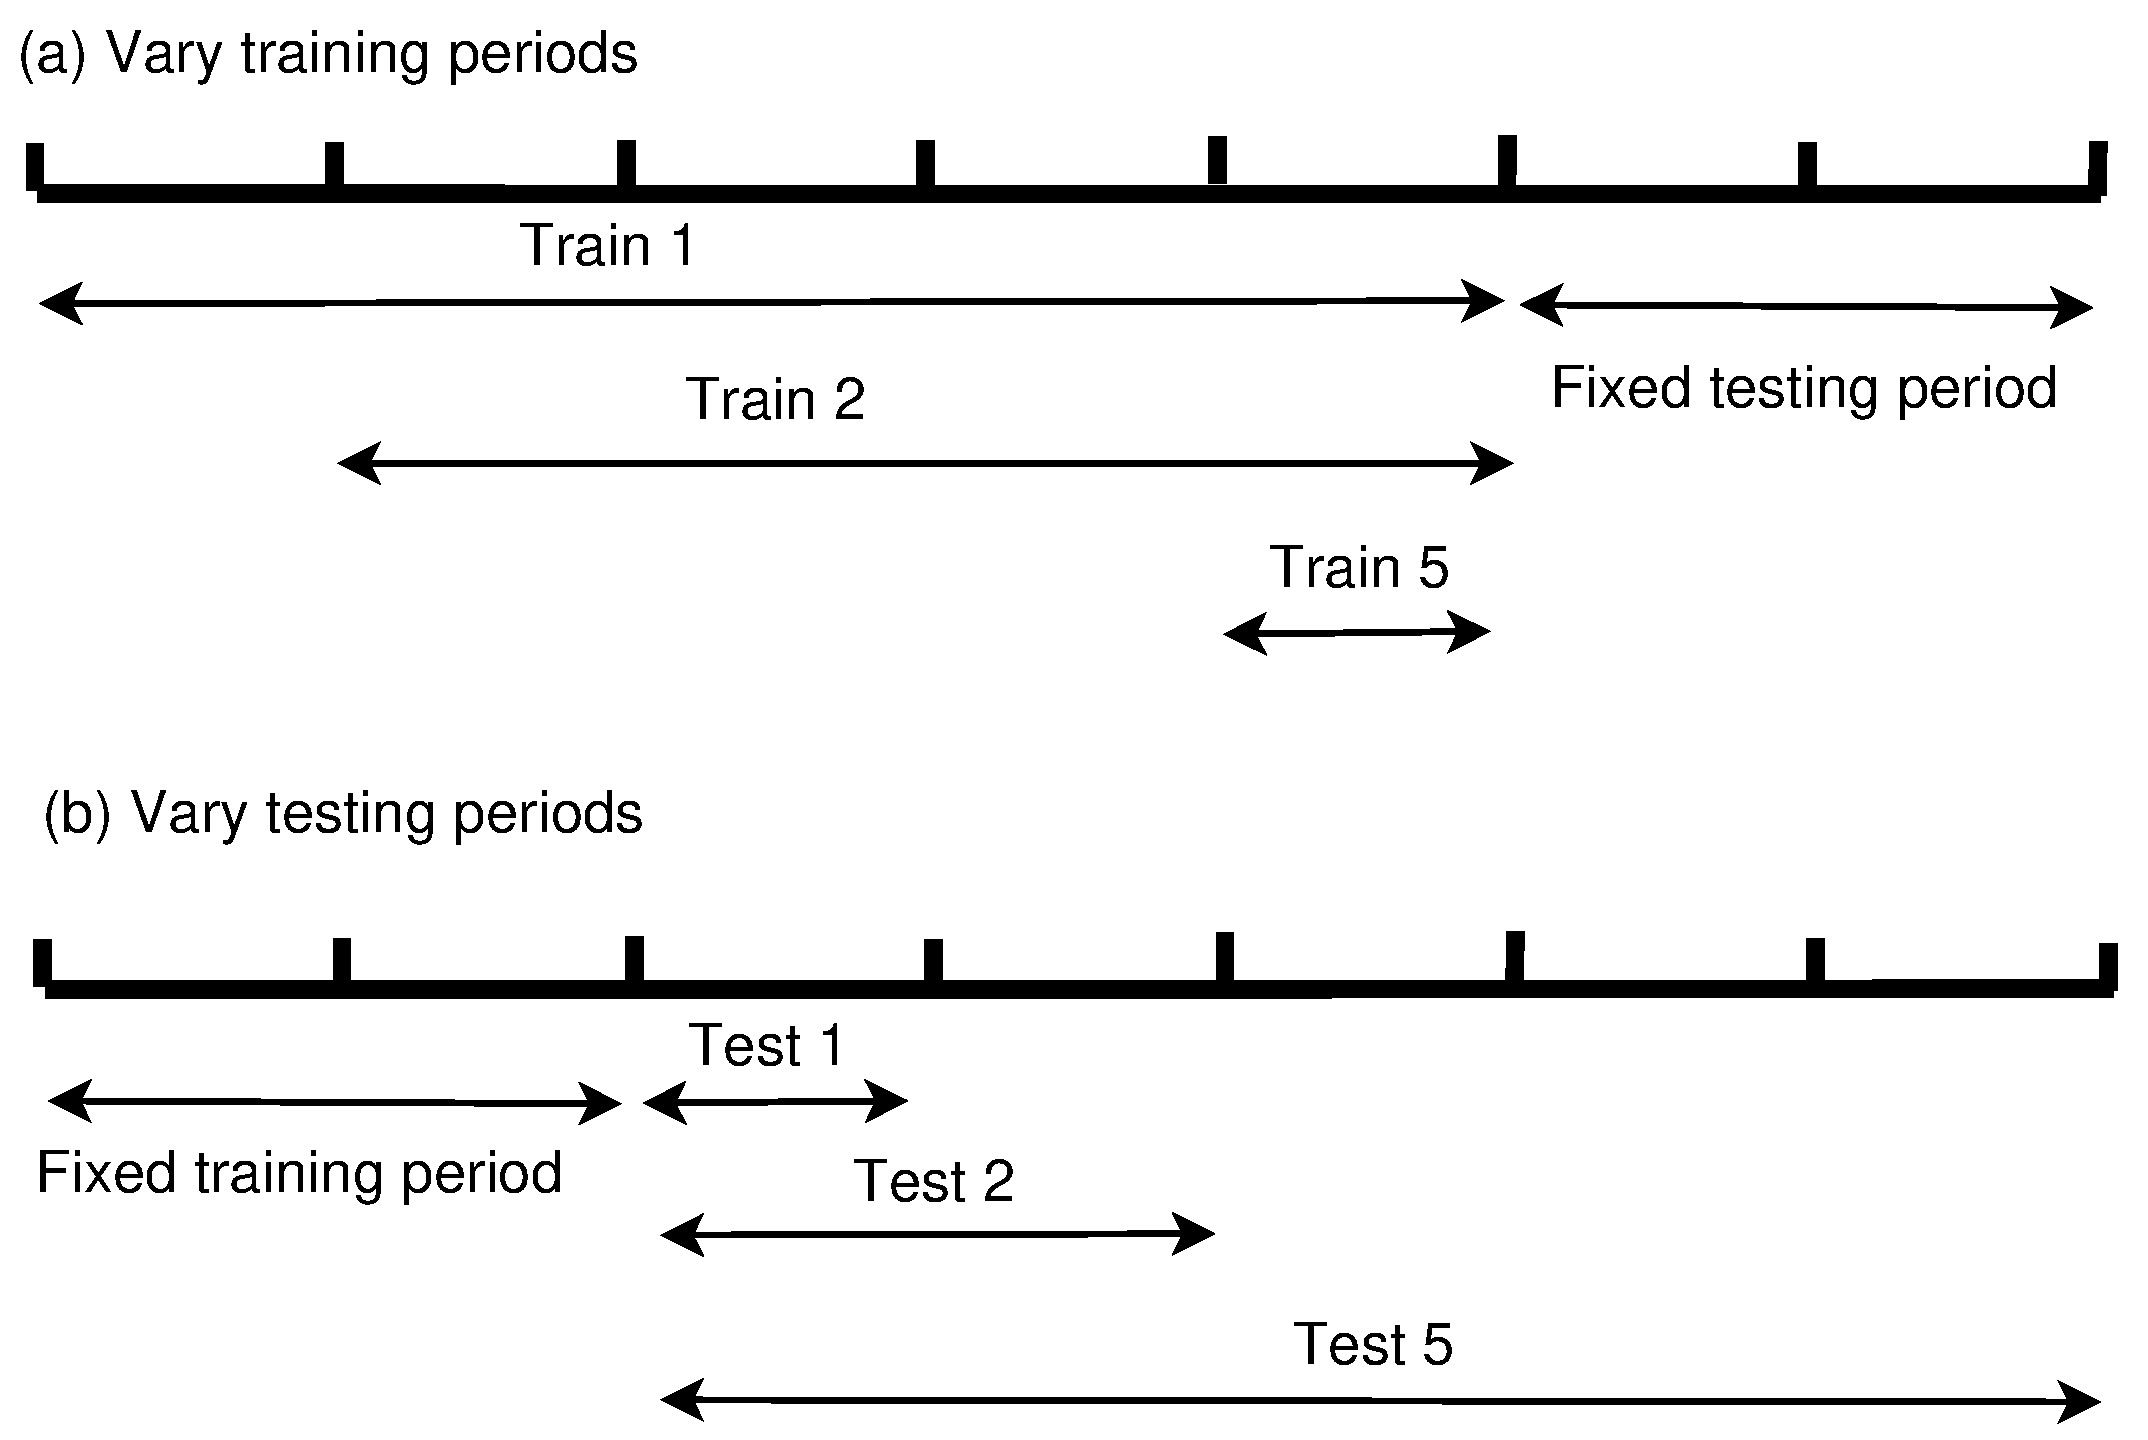
\includegraphics[width=0.75\linewidth]{FileAccess/figs/traintestsplits}
\caption{Splitting dataset into various training and testing periods
%The training period is used for feature extraction and model
%training, and the testing period is used for evaluation of the
%trained models.
} 
\label{fig:traintestsplits}
\end{center}
\end{figure}
%%
We divide the total duration of data from each share into several
slices and create training and testing periods such that testing
occurs immediately after training. For consistency, each share is
divided into seven slices and five training and five testing periods
are created as shown in Figure~\ref{fig:traintestsplits}.
We perform experiments with different combinations:
\begin{itemize}
  \renewcommand{\labelitemi}{$\bullet$}
\item\textbf{Fix testing, vary training.}  A longer training window has
  more number of activities, thereby allowing better model training. 
 However the activities become older as the
  distance between them and the testing period increases, thus preventing the model from reflecting the latest user patterns accurately.  On the
  other hand, a small training window has less number of activities,
  but these activities are relatively fresh.  Thus, there exists a
  trade-off between the size and the \textit{recency} of the training data.
  We study this trade-off by varying the training duration, while
  keeping the testing period fixed.
\item\textbf{Fix training, vary testing.}  As a user's behavior
  evolves over time, it is expected that the effectiveness of the
  user's model would degrade as the testing period becomes longer.  We
  can measure the robustness of a model by observing the rate of
  degradation.  With this goal, we experiment with varying testing
  periods, while keeping the training period fixed.
\end{itemize}
%We next discuss the metrics used to evaluate the performance of our system. 

%% We divide the total duration of data from each share into several slices and create training and testing periods such that testing occurs immediately after training. For consistency, each share is divided into seven slices and five training and five testing periods are created as shown in Figure~\ref{fig:traintestsplits}. 
%% %The total duration of data available from each share is divided into seven slices and several training and testing periods are created (Figure~\ref{fig:traintestsplits}). 
%% The following sets of experiments are conducted. %while ensuring the training and testing periods are adjacent to each other. 

%% \textbf{Fix testing, vary training.}  Given a testing period, a shorter and hence \textit{nearer} training period uses more recent activity however the amount of training data is less. We study this trade-off in model performance by varying the training duration and keeping the testing period fixed. 

%% \textbf{Fix training, vary testing.} Since user behavior may evolve over time, it is expected that the accuracy of trained models would degrade as testing a longer duration. We validate this intuition by fixing the training period and varying testing periods. 

%% %We next discuss the metrics used to evaluate the performance of our system. 

\subsubsection{Evaluation metrics}
\label{sec:metrics}
%%
Consider an experiment with a certain combination of training and
testing periods for a user $u$.  Let $F_{true +, u}$ denote the set of
files that $u$ accessed in the testing period, and $F_{pred +, u}$
denote the set of files predicted by $u$'s model.  Then the precision
and the recall of the model respectively are $\frac{\mid F_{true +, u}
  \cap F_{pred +, u} \mid}{\mid F_{pred +, u}\mid }$, and $\frac{\mid F_{true +,
    u} \cap F_{pred +, u} \mid}{\mid F_{true +, u}\mid}$.  We use the following
metrics to evaluate the effectiveness of the model.
\begin{itemize}
  \renewcommand{\labelitemi}{$\bullet$}
\item \textbf{F-score}: The F-score for a model is the harmonic mean
  of the precision and the recall, and provides a balanced picture of
  the model's effectiveness.
\item \textbf{Recall@75P}: In practice, it is important for a
  recommendation system to have high precision because a large number
  of false positives may discourage a user from using the system
  altogether.  Therefore, we additionally measure the recall values
  when the precision is high -- 75\%.  This is achieved with the help
  of confidence scores associated with the predicted labels.
\end{itemize} 
The measurements for F-score and Recall@75P are averaged across all
the evaluation users to obtain AF and AR@75P respectively. For each
share, we report the average and the maximum values of AF and AR@75P
across the results over all combinations of training and testing
periods.  Please note that the maximum values provide realistic
performance estimate of a properly tuned system.

%% For a certain training period, a testing period and a user $u$, let $F_{true +, u}$ denote the set of files that $u$ read in testing period, and $F_{pred +, u}$ denote the set of files that the model for $u$ predicts would be accessed by $u$. The precision of the predictions made by the model for $u$ is equal to $\frac{\mid F_{true +, u} \cap F_{pred +, u} \mid}{F_{pred +, u}}$ and the recall is equal to $\frac{\mid F_{true +, u} \cap F_{pred +, u}  \mid}{F_{true +, u}}$. We use the following metrics to evaluate the correctness of trained user models in our system. 
%% \begin{itemize}
%% \item \textbf{F-score}: The F-score for user $u$ is the harmonic mean of the precision and recall for the model of $u$ and provides a balanced picture of the prediction correctness. 
%% \item \textbf{Recall@75P}: Practically, it is important for a recommendation system to have high precision since a large number of false positives in the recommendations may discourage the user from using the system altogether. Therefore, with the help of confidence scores associated with each test file, we set the precision to a high value and also evaluate the system based on its recall when precision is 75\%. 


%% \end{itemize} 
%% The F-score and Recall@75P are averaged across the evaluation users to obtain AF and AR@75P respectively. For each share, we report the average as well as the maximum values of AF and AR@75P across all training and testing periods. The maximum values can provide a realistic estimate of the performance expected from a properly tuned system. 

\section{Performance Evaluation} 
\label{sec:results} 
%%
We evaluate our system using the Python-based scikit-learn
library~\cite{scikit-learn}.  We train models on a 32 core, 64GB,
2.6GHz machine, and conduct testing on a separate 8 core, 32GB, 2.7GHz
machine, leveraging multiple cores with multiprocessing.  We use
3-fold cross-validation to learn the regularization parameter $C$ for
the linear SVM models by varying $C$ over {$\{10^{-2}, 10^{-1}, 1,
  10^{1}, 10^{2}, 10^{3}\}$}.

%% The evaluation of our system is conducted using Python-based scikit-learn library~\cite{scikit-learn}. Training of the models is done on a 32 core, 64GB, 2.6GHz machine where the implementation uses multiprocessing to divide computation load across multiple cores. The testing is done on a 8 core, 32GB, 2.7GHz machine. 
%% %\indent Linear Support Vector Machines (SVMs) are chosen to model user access patterns since they offer high model correctness for low training times \cite{dwiticeis15}. In addition, linear SVMs provide feature weights that can determine the significance of individual features, and can be leveraged for techniques such as Active Feature based Model Selection (Section~\ref{sec:testspeedup}) to significantly reduce testing computation of our system. 
%% We use 3-fold cross-validation to learn the regularization parameter $C$ for the linear SVM models by varying $C$ over {$\{10^{-2},
%%   10^{-1}, 1, 10^{1}, 10^{2}, 10^{3}\}$}.  
%\vspace{-0.2in}
%%
\subsection{Metadata Models} 
\begin{table*}[t!]
{\fontsize{8pt}{1em}\selectfont
\begin{center}
\caption{Performance summary for metadata models.  Performance
  numbers are averaged over 5 iterations with random
  initialization of the linear SVM model training. Numbers are listed
  along with the standard deviations. }
%\begin{tabular}{|p{0.6cm}|@{\hspace{0.05in}}p{1.2cm}|@{\hspace{0.03in}}p{1.2cm}|@{\hspace{0.03in}}p{1.2cm}|@{\hspace{0.03in}}p{1.2cm}|>{\raggedleft}p{1.2cm}|}
\begin{tabular}{|c|r|r|r|r|r|}
		\hline
		\textbf{Share} & \textbf{Avg AF} & \textbf{Max AF} & \textbf{Avg AR@75P} & \textbf{Max AR@75P} & \textbf{\% TP by others} \tabularnewline
		\hline
%A&\textbf{37.7}$\pm$0.0&\textbf{40.3}$\pm$0.0&\textbf{0.8}$\pm$0.0&\textbf{1.6}$\pm$0.2&\textbf{84}$\pm$0.0\tabularnewline \hline
A&\textbf{80.7}$\pm$0.0&\textbf{91.1}$\pm$0.0&\textbf{77.6}$\pm$0.0&\textbf{93.9}$\pm$0.0&\textbf{20.4}$\pm$0.0\tabularnewline \hline
B&\textbf{46.4}$\pm$0.0&\textbf{51.2}$\pm$0.0&\textbf{34.9}$\pm$0.0&\textbf{44.2}$\pm$0.0&\textbf{73.1}$\pm$0.0\tabularnewline \hline
C&\textbf{23.1}$\pm$0.0&\textbf{24.2}$\pm$0.0&\textbf{11.4}$\pm$0.0&\textbf{12.4}$\pm$0.0&\textbf{87.7}$\pm$0.0\tabularnewline \hline
D&\textbf{30.7}$\pm$0.0&\textbf{36.3}$\pm$0.0&\textbf{19.0}$\pm$0.0&\textbf{24.7}$\pm$0.0&\textbf{82.8}$\pm$0.0\tabularnewline \hline
E&\textbf{26.9}$\pm$0.0&\textbf{35.0}$\pm$0.0&\textbf{17.9}$\pm$0.0&\textbf{24.1}$\pm$0.0&\textbf{66.0}$\pm$0.0\tabularnewline \hline
F&\textbf{81.5}$\pm$0.0&\textbf{84.3}$\pm$0.0&\textbf{82.9}$\pm$0.0&\textbf{84.6}$\pm$0.0&\textbf{9.8}$\pm$0.0\tabularnewline \hline
G&\textbf{44.8}$\pm$0.0&\textbf{51.3}$\pm$0.0&\textbf{50.6}$\pm$0.0&\textbf{58.3}$\pm$0.0&\textbf{99.9}$\pm$0.0\tabularnewline \hline
H&\textbf{47.6}$\pm$0.0&\textbf{50.2}$\pm$0.0&\textbf{49.9}$\pm$0.0&\textbf{53.0}$\pm$0.0&\textbf{74.4}$\pm$0.0\tabularnewline \hline
%J&\textbf{26.6}$\pm$0.0&\textbf{27.2}$\pm$0.0&\textbf{4.7}$\pm$0.0&\textbf{5.8}$\pm$0.0&\textbf{79}$\pm$0.0\tabularnewline \hline
\end{tabular}
\end{center}
%\vspace{-0.35in}
\label{tab:WithoutBurstsPerf} % Note: these are latest. -2/26/15
}
\end{table*}
\begin{table*}[t!]
{\fontsize{8pt}{1em}\selectfont
\begin{center}
\caption{Performance summary for CF models. Performance
  numbers are averaged over 5 iterations with random
  initialization of the linear SVM model training. Numbers are listed
  along with the standard deviations.}
%\begin{tabular}{|p{0.6cm}|@{\hspace{0.05in}}p{1.2cm}|@{\hspace{0.03in}}p{1.2cm}|@{\hspace{0.03in}}p{1.2cm}|@{\hspace{0.03in}}p{1.2cm}|>{\raggedleft}p{1.2cm}|}
\begin{tabular}{|c|r|r|r|r|r|}
		\hline
		\textbf{Share} & \textbf{Avg AF} & \textbf{Max AF} & \textbf{Avg AR@75P} & \textbf{Max AR@75P} & \textbf{\% TP by others} \tabularnewline
		\hline
%A&\textbf{37.4}$\pm$0.1&\textbf{46.1}$\pm$0.0&\textbf{0.5}$\pm$0.0&\textbf{2.6}$\pm$0.0&\textbf{82}$\pm$0.0\tabularnewline \hline
A&\textbf{80.7}$\pm$0.0&\textbf{100.0}$\pm$0.0&\textbf{78.5}$\pm$0.0&\textbf{100.0}$\pm$0.0&\textbf{21.2}$\pm$0.0\tabularnewline \hline
B&\textbf{48.6}$\pm$0.0&\textbf{77.1}$\pm$0.0&\textbf{32.2}$\pm$0.6&\textbf{62.1}$\pm$0.0&\textbf{73.1}$\pm$0.0\tabularnewline \hline
C&\textbf{23.5}$\pm$0.0&\textbf{36.0}$\pm$0.0&\textbf{10.1}$\pm$0.0&\textbf{16.0}$\pm$0.0&\textbf{87.5}$\pm$0.0\tabularnewline \hline
D&\textbf{32.3}$\pm$0.0&\textbf{47.5}$\pm$0.0&\textbf{21.5}$\pm$0.0&\textbf{38.3}$\pm$0.0&\textbf{83.3}$\pm$0.0\tabularnewline \hline
E&\textbf{27.6}$\pm$0.0&\textbf{41.1}$\pm$0.0&\textbf{25.3}$\pm$0.0&\textbf{100.0}$\pm$0.0&\textbf{65.7}$\pm$0.0\tabularnewline \hline
F&\textbf{81.5}$\pm$0.0&\textbf{87.9}$\pm$0.0&\textbf{83.3}$\pm$0.0&\textbf{89.2}$\pm$0.0&\textbf{9.8}$\pm$0.0\tabularnewline \hline
G&\textbf{55.5}$\pm$0.1&\textbf{76.2}$\pm$0.0&\textbf{58.0}$\pm$0.2&\textbf{89.9}$\pm$0.4&\textbf{96.6}$\pm$0.1\tabularnewline \hline
H&\textbf{47.6}$\pm$0.0&\textbf{57.2}$\pm$0.0&\textbf{49.6}$\pm$0.0&\textbf{66.5}$\pm$0.0&\textbf{75.4}$\pm$0.0\tabularnewline \hline
%J&\textbf{26.7}$\pm$0.0&\textbf{28.7}$\pm$0.0&\textbf{2.9}$\pm$0.0&\textbf{5.6}$\pm$0.0&\textbf{79}$\pm$0.0\tabularnewline \hline
\end{tabular}
\end{center}
}
%\vspace{-0.1in}

\label{tab:CollabFilteringPerf}  % Note: these are latest. -2/26/15 
\end{table*}

Table~\ref{tab:WithoutBurstsPerf} shows performance results of the
metadata models.  The numbers in column Max AR@75P are reasonable
performance estimate of a well tuned system.  The average of these
numbers across all the shares, 49.4\%, shows that our metadata models 
can capture nearly half of users' access for new files, while having under 25\% 
wrong file recommendations. This demonstrates the effectiveness of the 
trained models. 

We would like to point out that our dataset includes an undesirable
case where during the testing phase, a user accesses a new file that 
was recently created by the same user. Since recommending such a file to the
user is not useful, we measure their proportion in our recommendations. 
The last column of Table~\ref{tab:WithoutBurstsPerf} shows that 
most of the correctly recommended files do not fall in the above category, 
thereby upholding the validity of our models.

%% Table~\ref{tab:WithoutBurstsPerf} shows that the performance of the metadata models varies significantly with the evaluation shares. Intuitively, it may not be useful to recommend a file to a user if the file had been recently created by the same user. The last column of Table~\ref{tab:WithoutBurstsPerf} shows that most of the files that are correctly recommended to users do not fall in this category. 

\subsection{CF Models} 
%%
We experimented with different strategies to sample validation files
for training CF models.  We use the strategy that provides the best
performance, which is using the training set itself as the validation
set.  The results in Table~\ref{tab:CollabFilteringPerf} clearly
highlight the significant gains of CF models over metadata models.
The average of Max AR@75P across all shares is 70.2\%, which is an
improvement of a whopping 20\% over the performance of metadata models.
Also, it is not very surprising that the top four shares, B, D, E, and
G, in terms of gains of the CF model, are found in the top five shares in
terms of normalized triangle counts.  Share A, which is the remaining
share in the top five, doesn't show substantial improvement primarily
because the performance of its metadata model is already too high.
%\vspace{-0.2in} 

%% We experimented with different strategies to sample validation files to train CF models. The best performance is observed when the set of validation files is the same as that of the training files. We have used this setting in our experiments. Table~\ref{tab:CollabFilteringPerf} shows that the CF models clearly outperform the metadata models. It can also be seen that most improvement after CF models is seen in shares B, D, E, and G which occur in the top five shares in Table~\ref{tab:datasetstats1} in terms of user collaboration as measured by normalized triangle counts. Although share A is among the top shares in terms of user collaboration, the performance of metadata models on share A is already high and so the improvement by CF models could not be substantial. 
%% %\vspace{-0.2in} 
\subsection{Temporal Variation in Performance}
%\vspace{-0.8cm}
\begin{figure*}
\centering
\begin{minipage}{.95\textwidth}
  \centering
  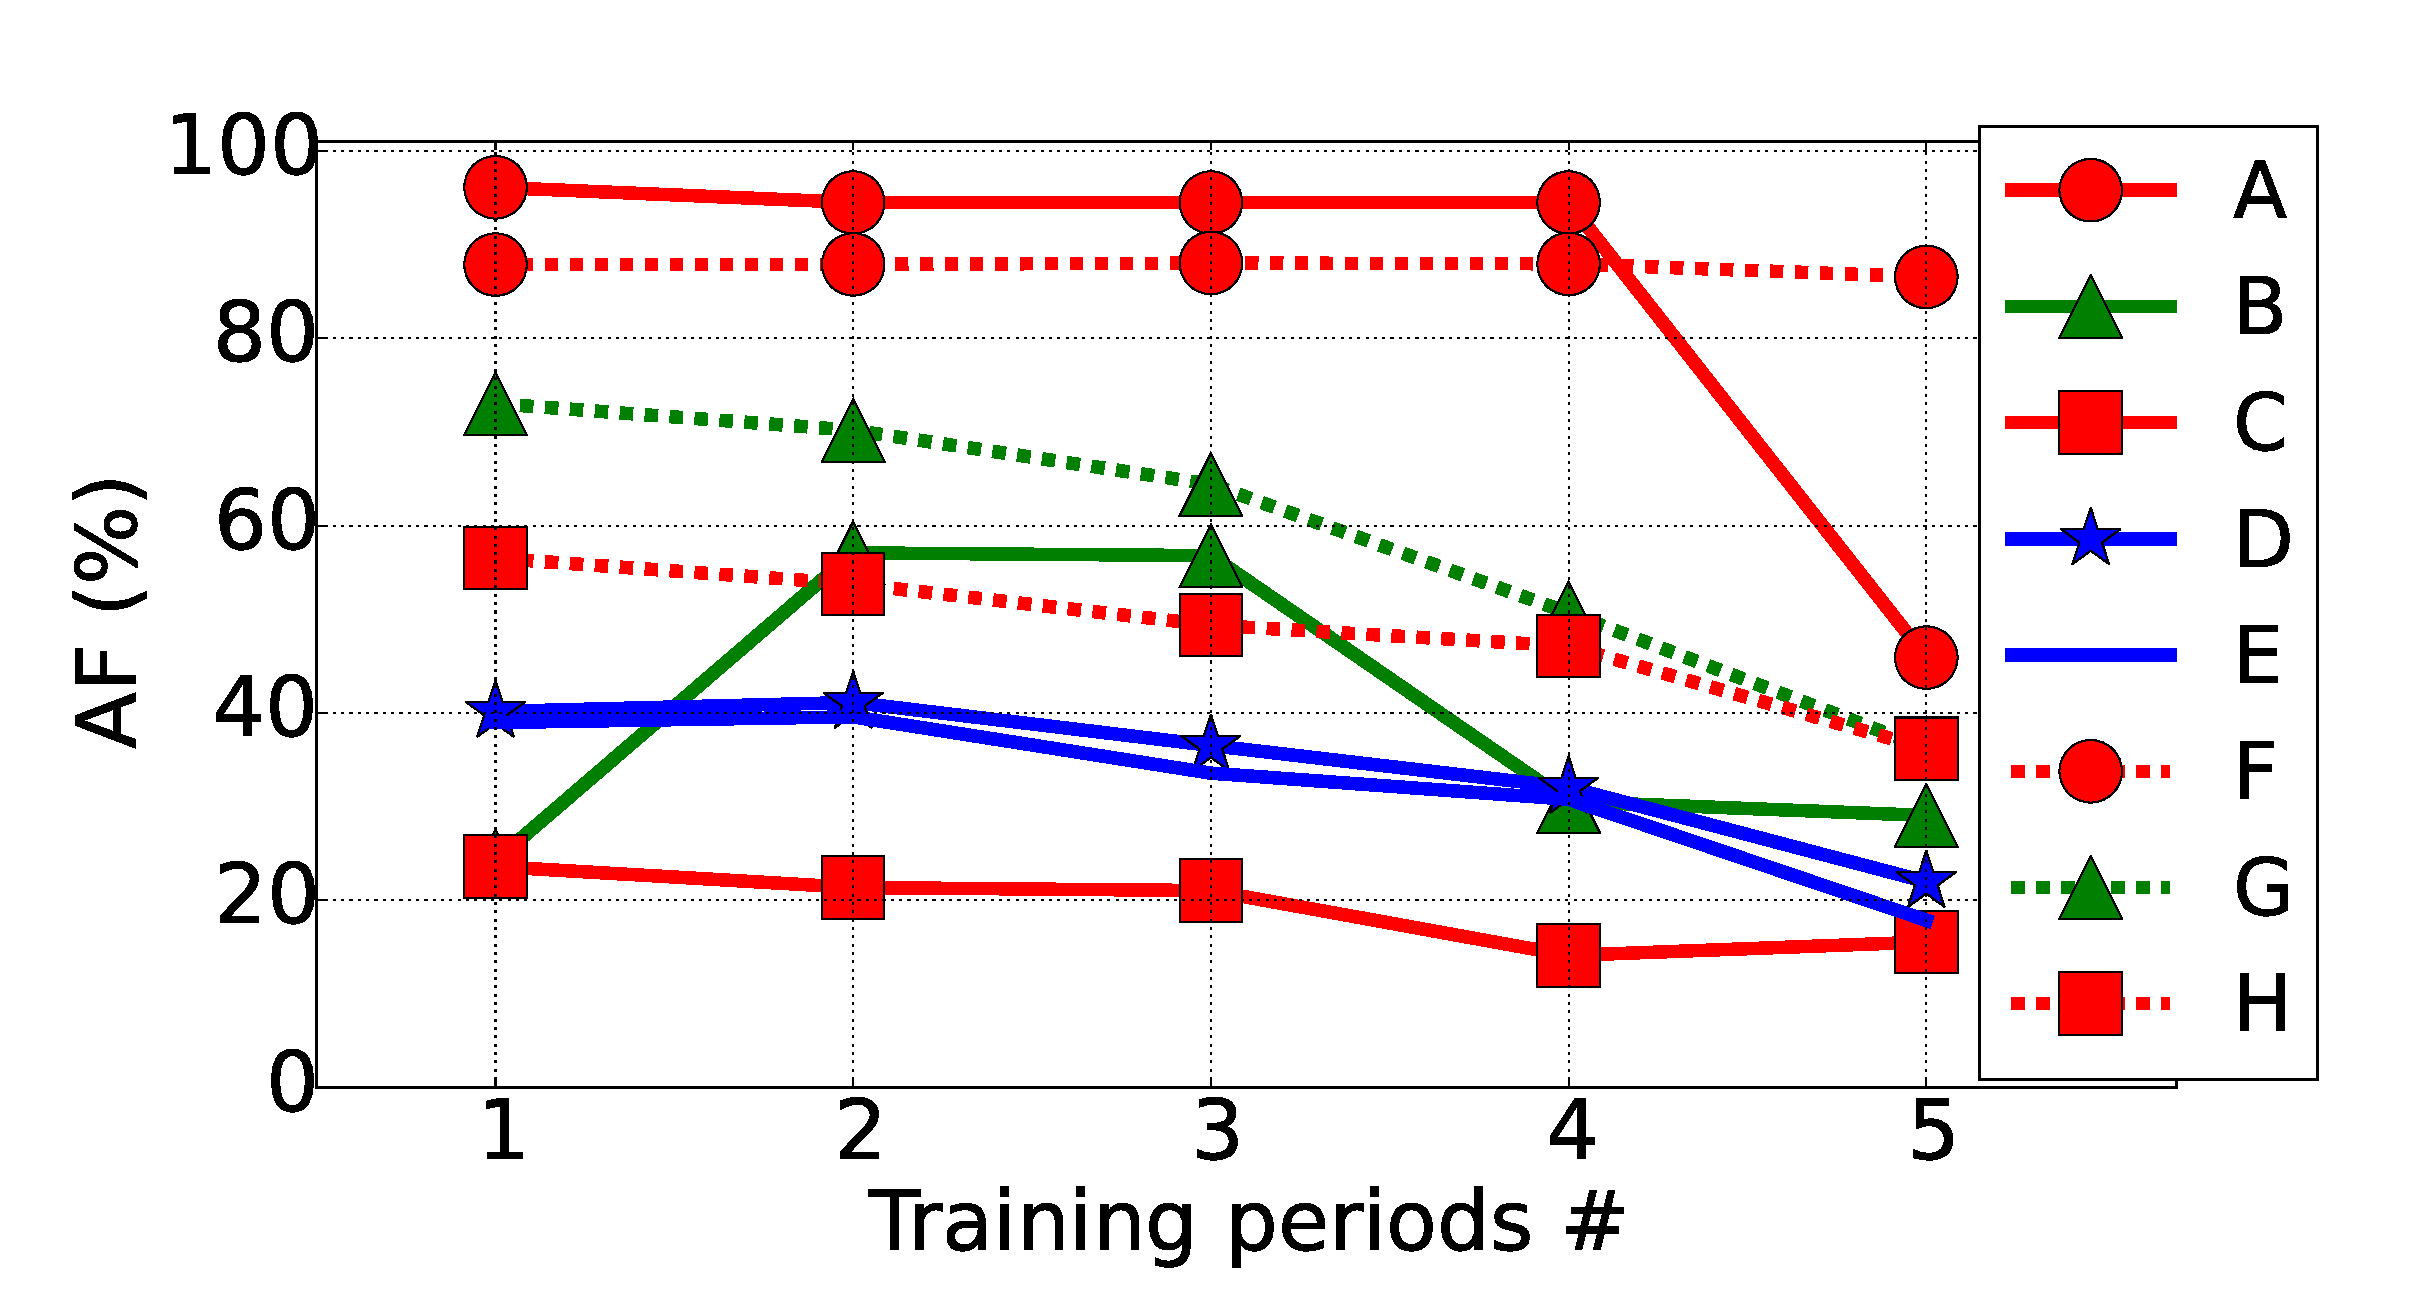
\includegraphics[width=0.65\linewidth]{FileAccess/figs/VaryTrainFScore10}
  \captionof{figure}{AF for metadata models with the fixed testing and varying training periods} 
  \label{fig:varytrainFscore}
%\vspace{-0.5cm}
\end{minipage} % 
\begin{minipage}{.95\textwidth}
  \centering
  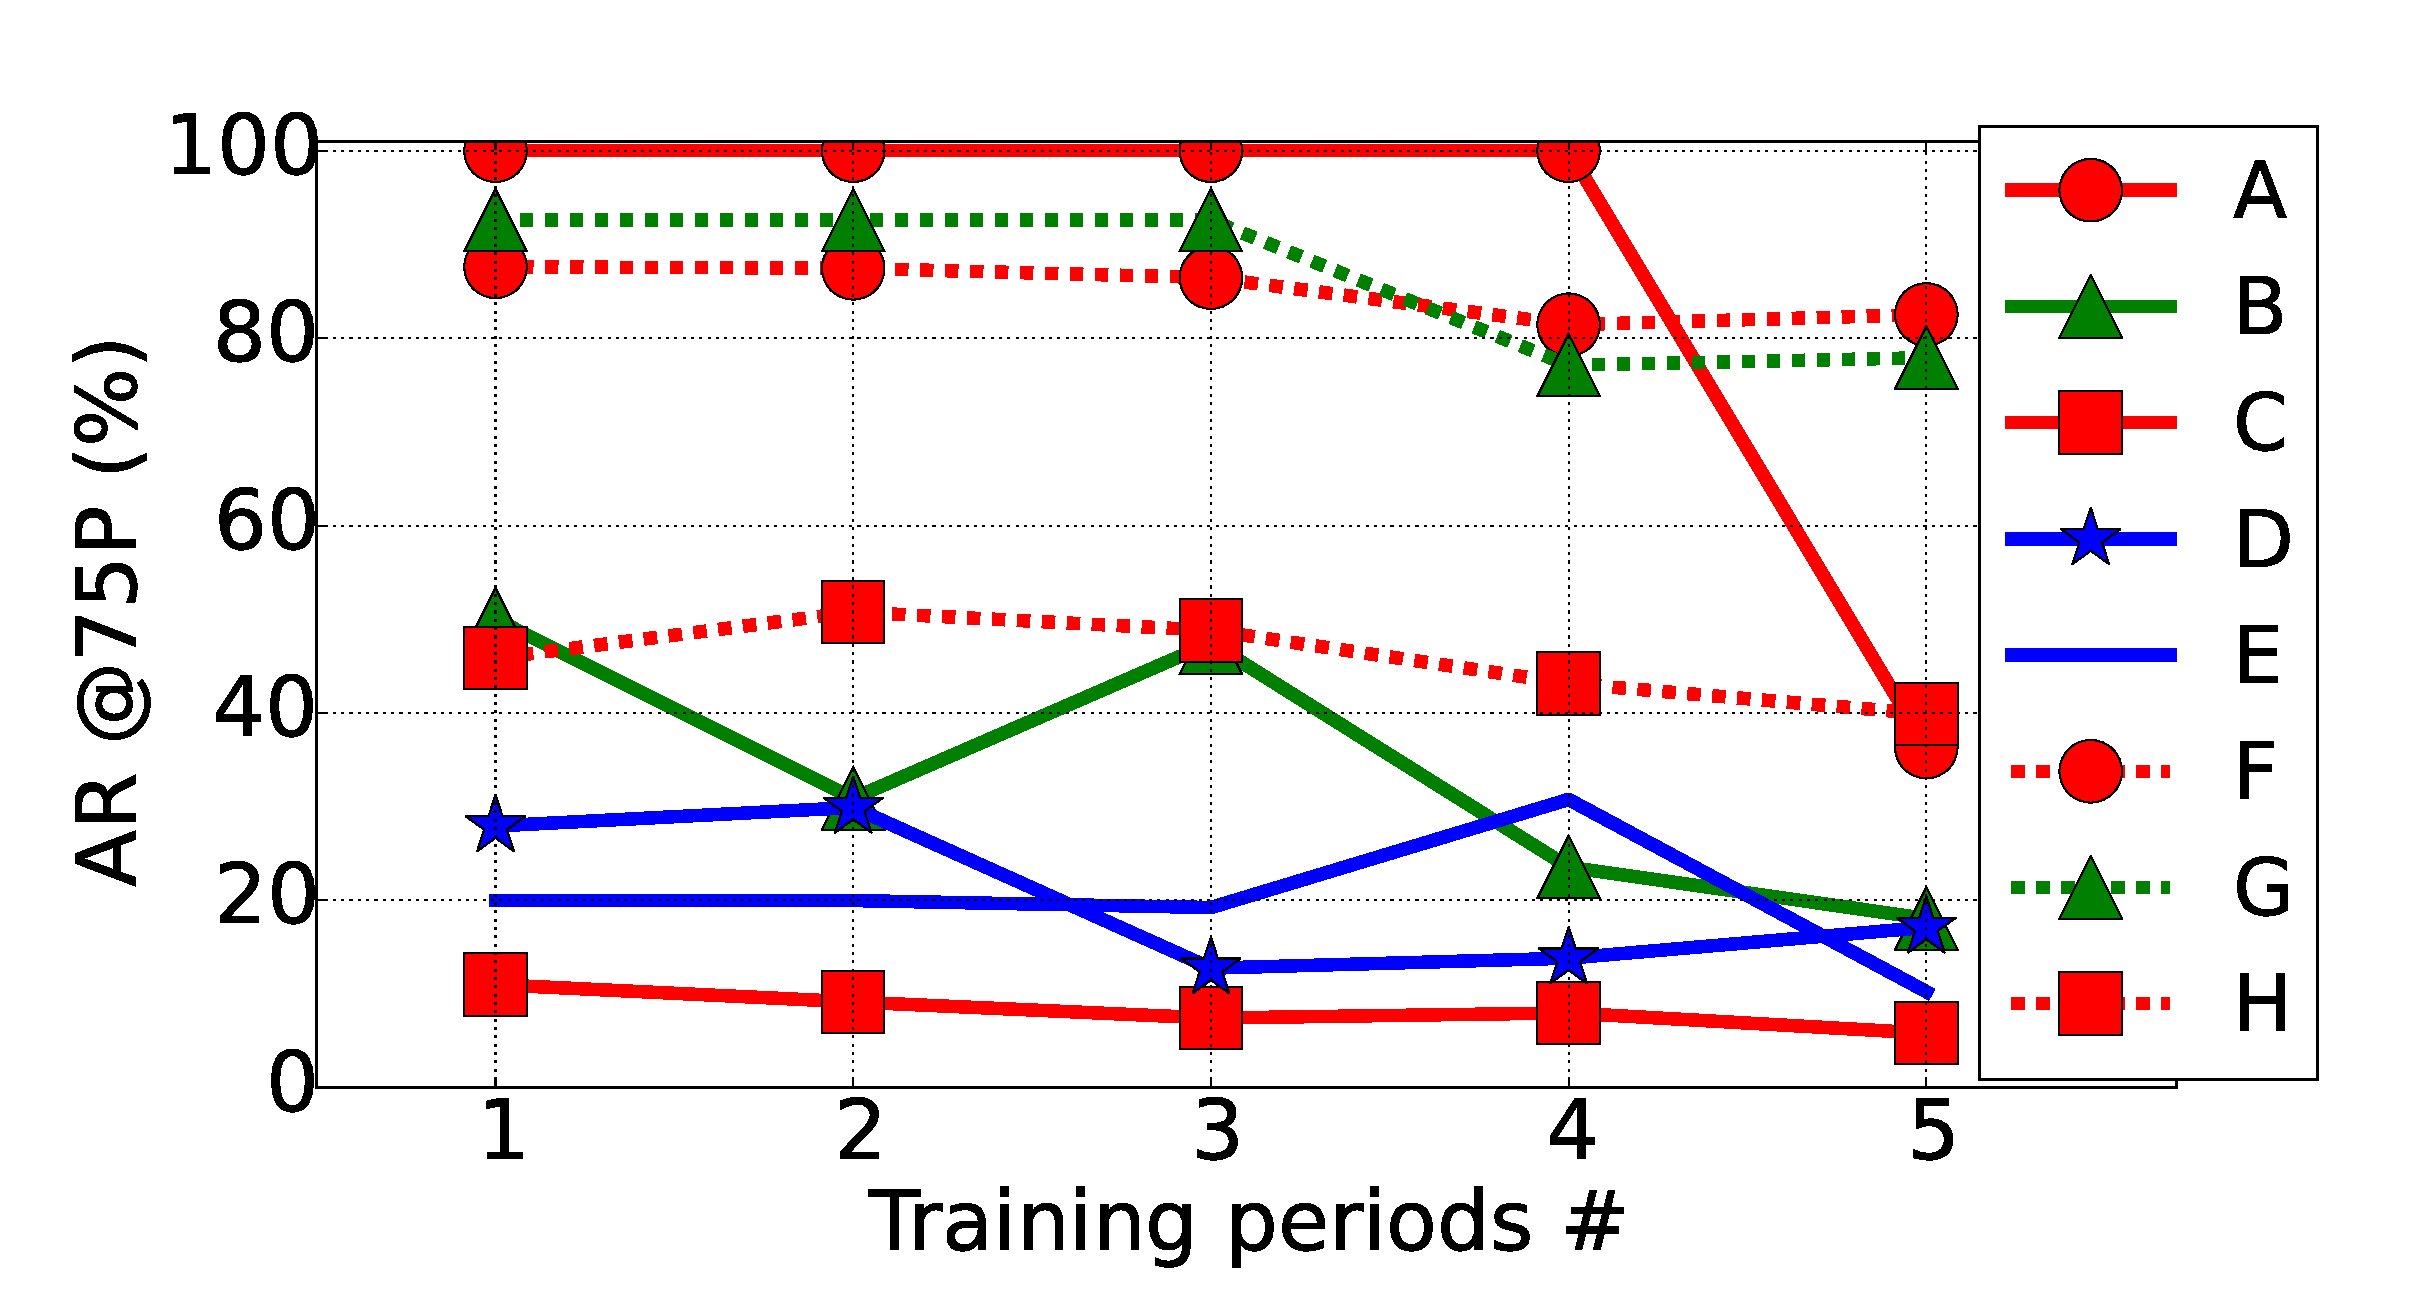
\includegraphics[width=0.65\linewidth]{FileAccess/figs/VaryTrainR7510}
  \captionof{figure}{AR@75P for metadata models with the fixed
    testing and varying training periods}
  \label{fig:varytrainR75}
%\vspace{-0.5cm}
\end{minipage}
\end{figure*}
%\vspace{-0.6cm}

\begin{figure*}
\centering
\begin{minipage}{.95\textwidth}
  \centering
  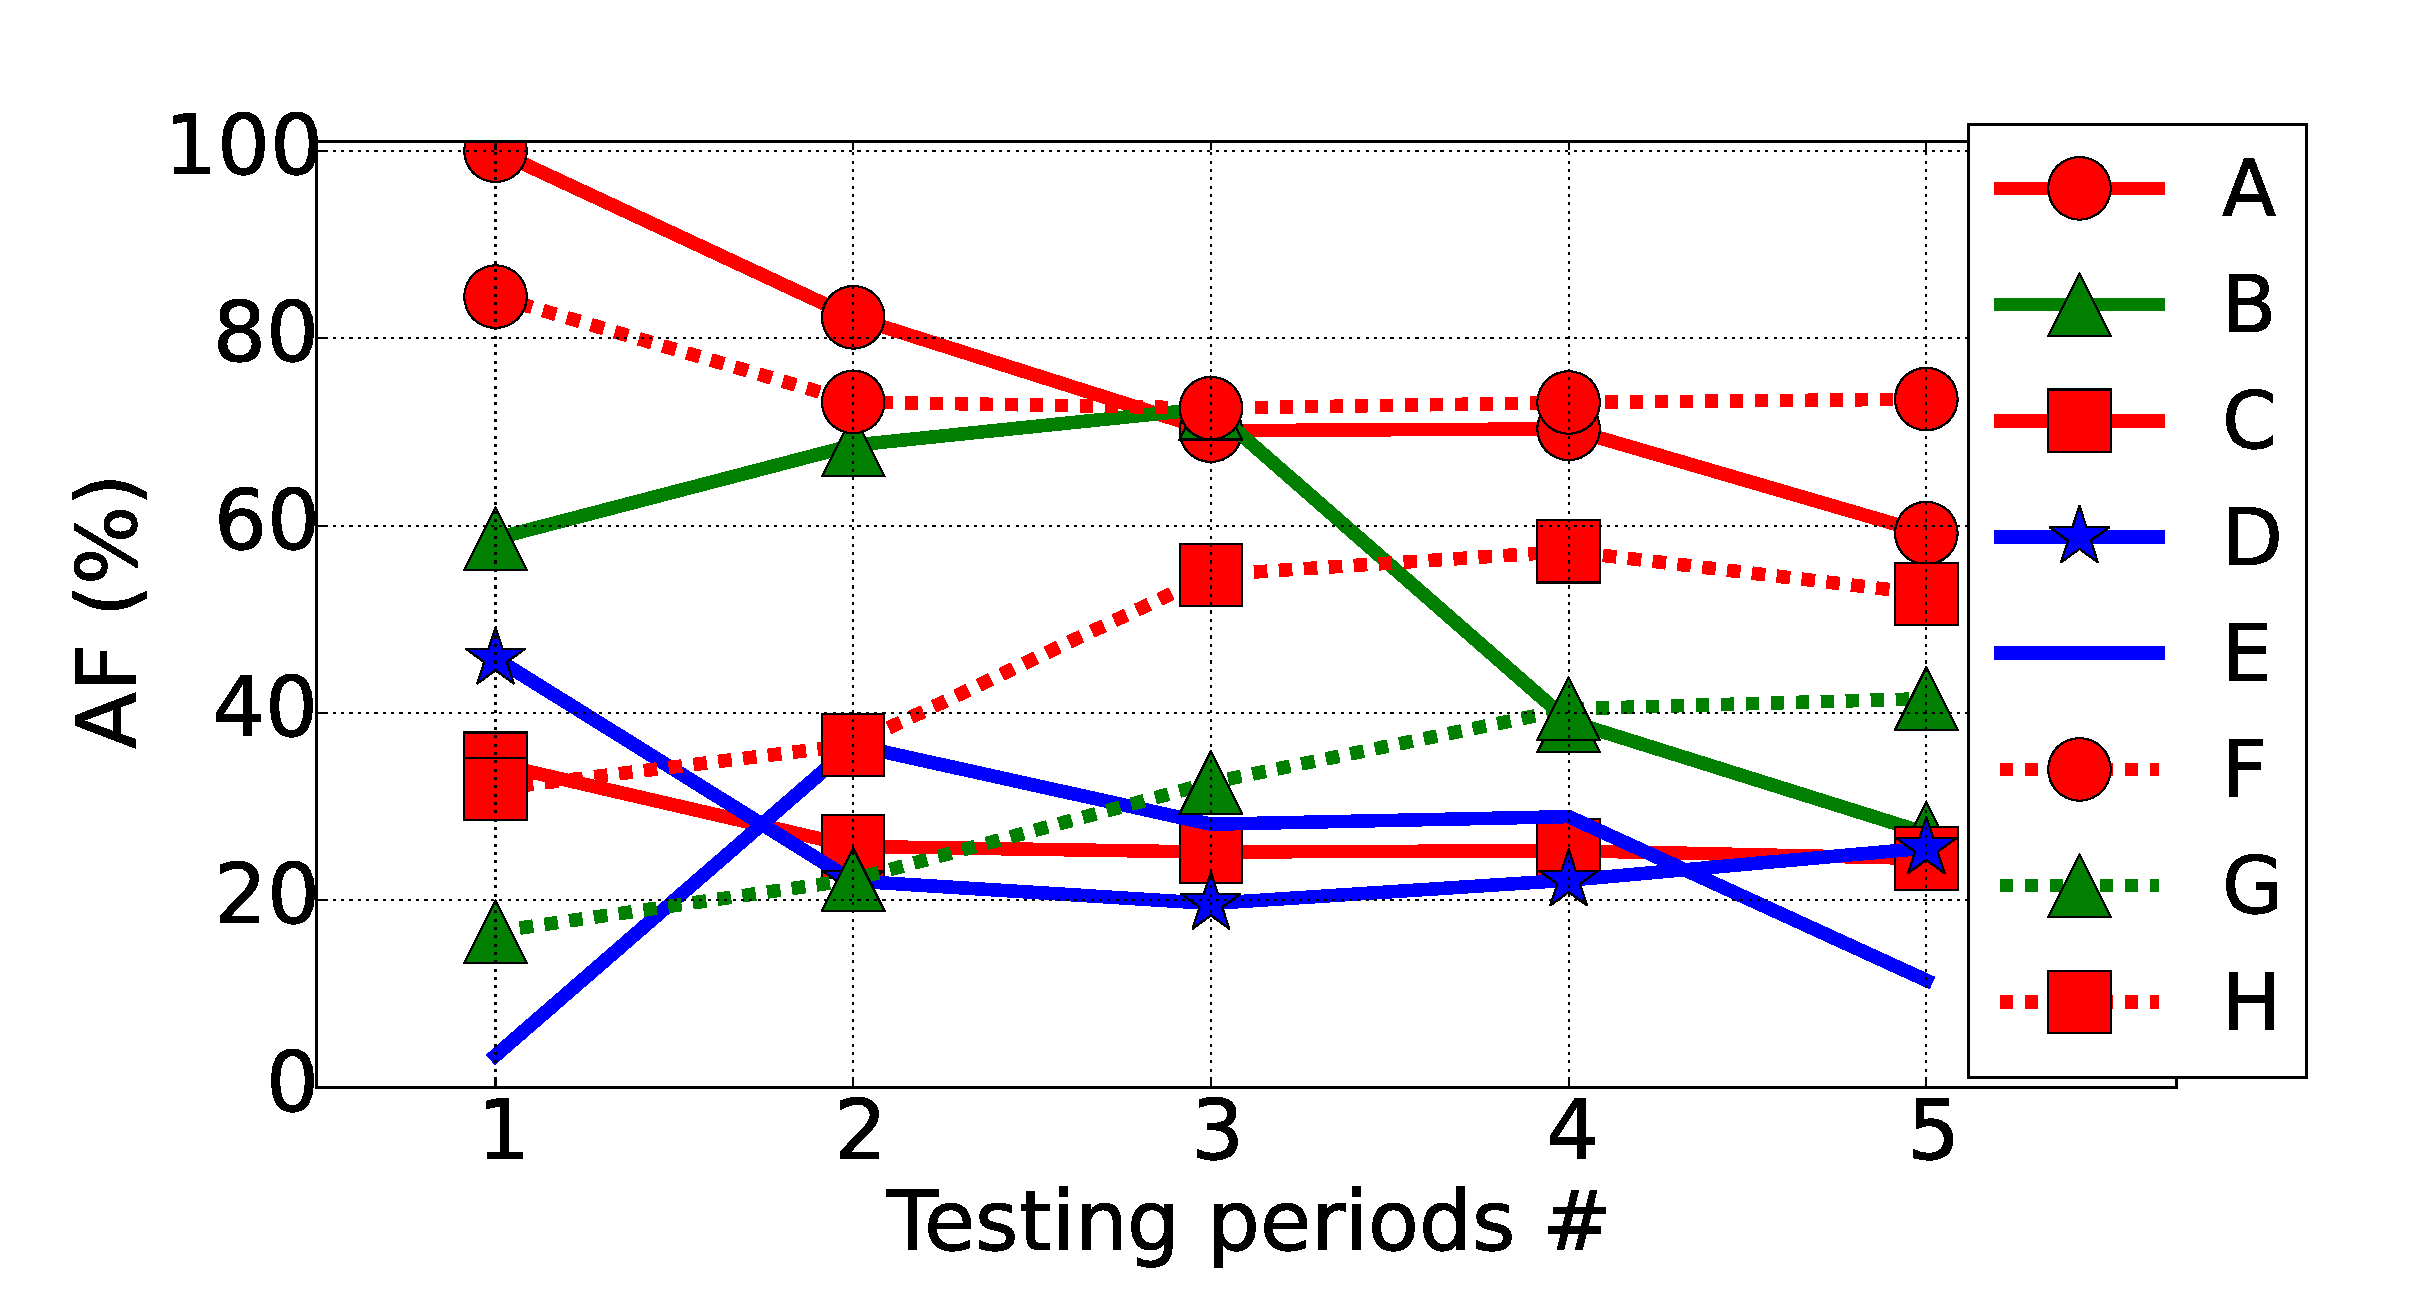
\includegraphics[width=0.65\linewidth]{FileAccess/figs/VaryTestFScore10}
  \captionof{figure}{AF for metadata models with the fixed 
    training and varying test periods}
  \label{fig:varytestFscore}
%\vspace{-0.2cm}
\end{minipage} %
\begin{minipage}{.95\textwidth}
  \centering
  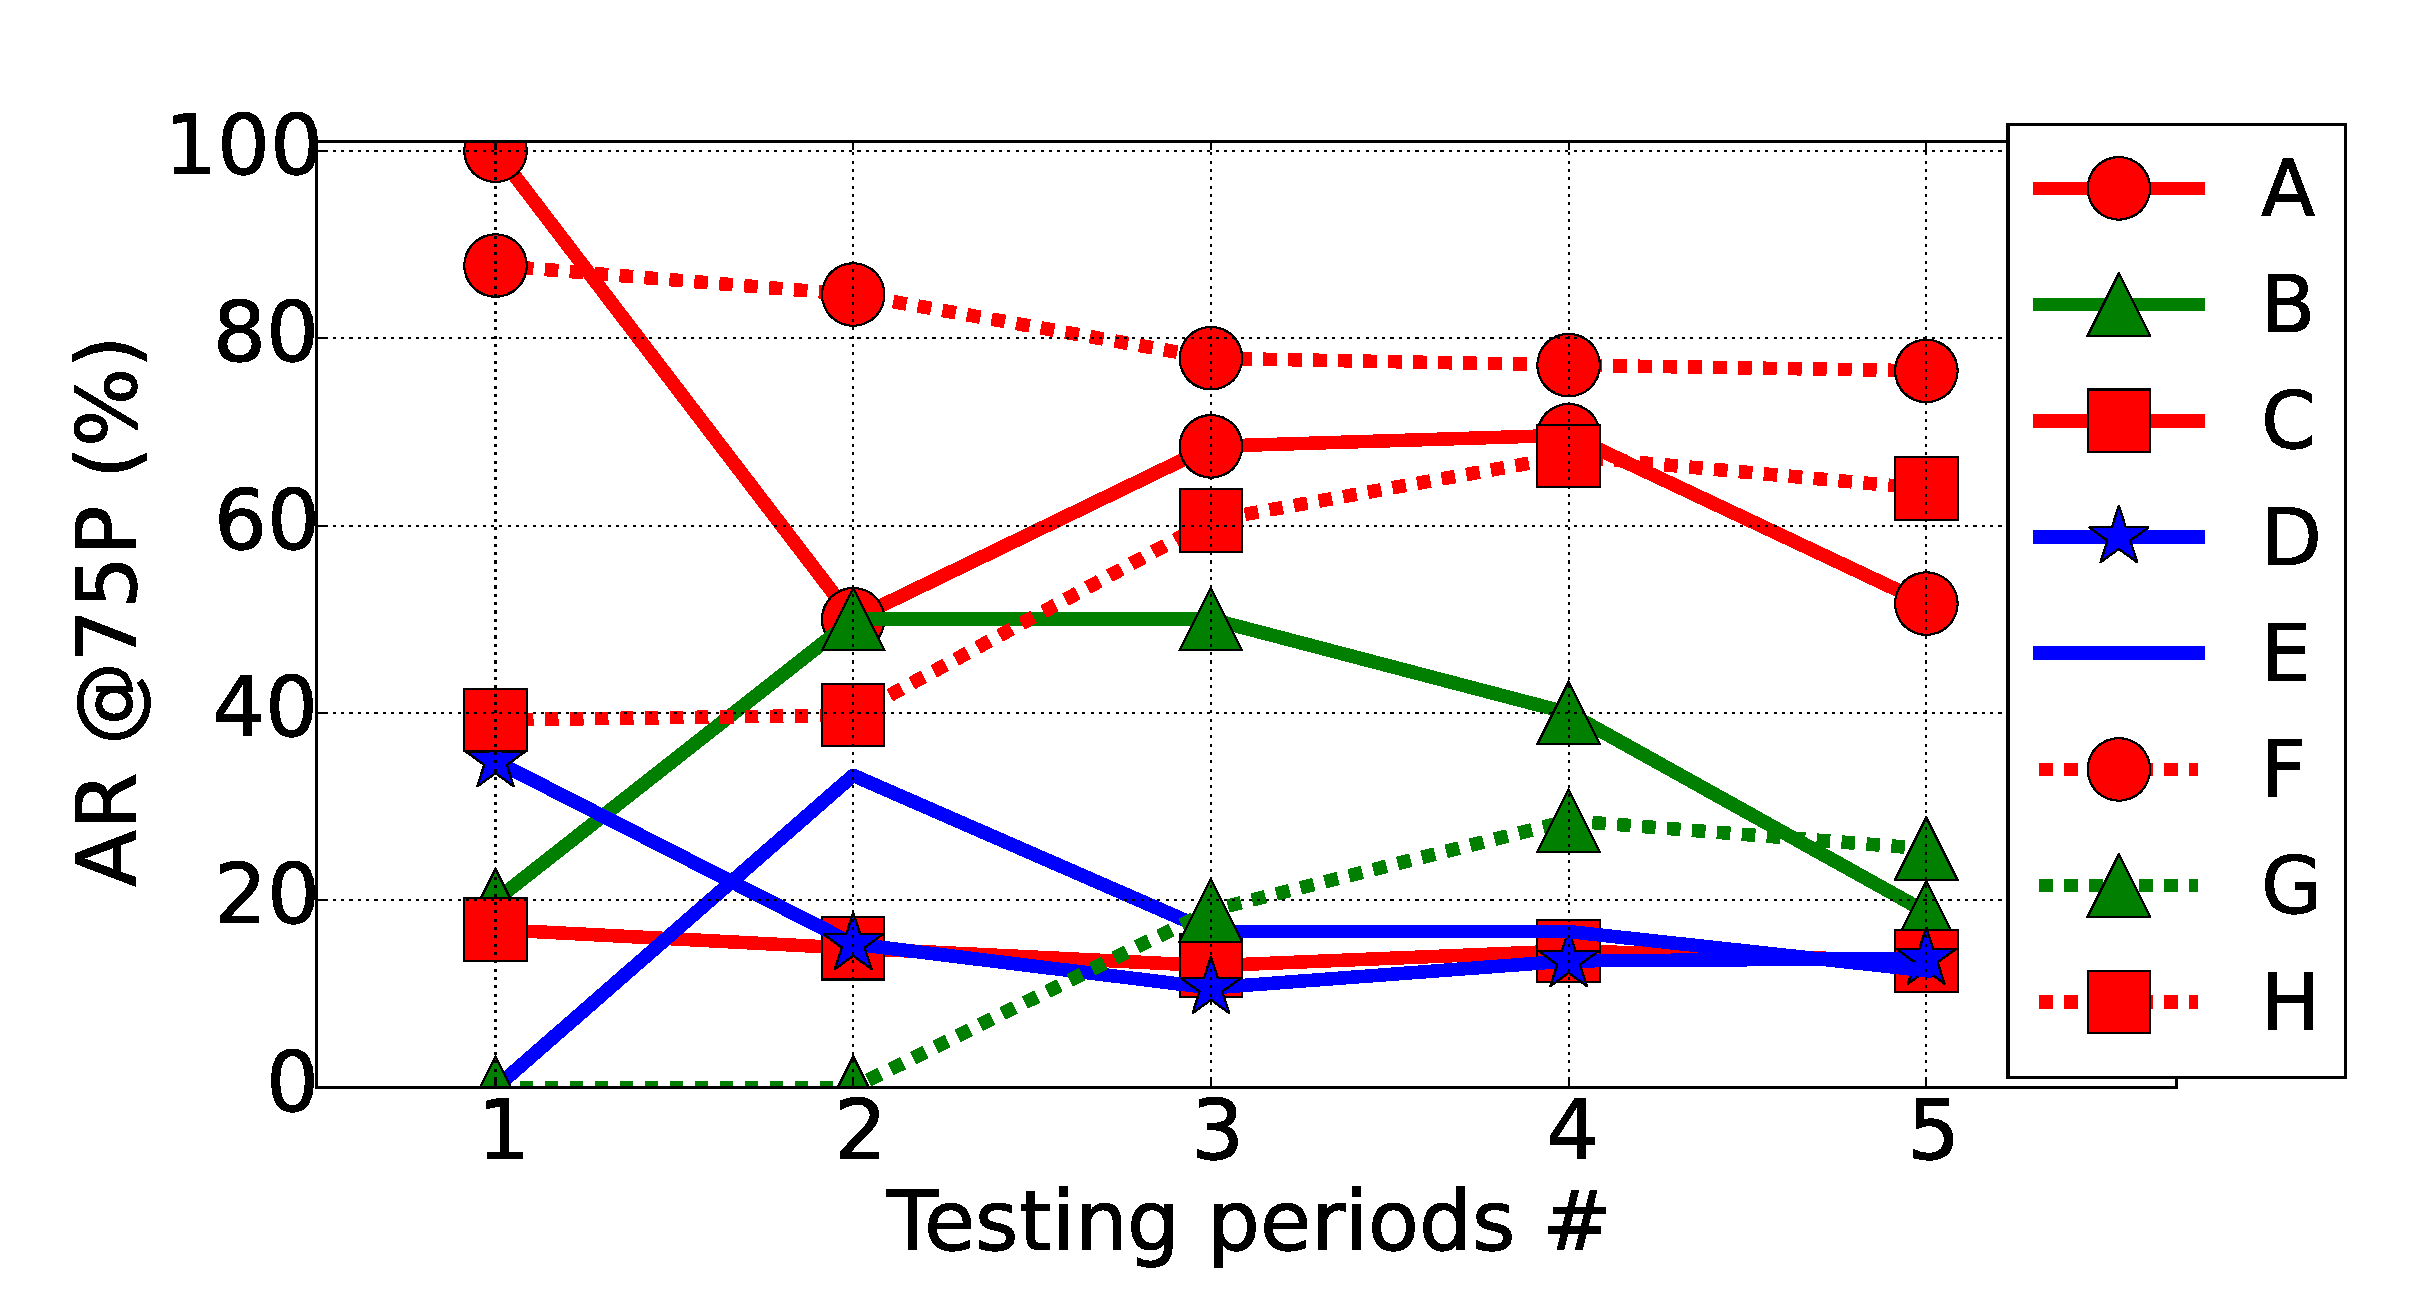
\includegraphics[width=0.65\linewidth]{FileAccess/figs/VaryTestR7510}
  \captionof{figure}{AR@75P for metadata models with the fixed
    training and varying test periods}
  \label{fig:varytestR75}
%\vspace{-0.2cm}
\end{minipage}
%\vspace{-0.1in}
\end{figure*}
%%
%%
To study the performance variations for different lengths of training
and testing periods, we focus only on the metadata models because as
compared to CF models, they provide larger variation owing to lower
baseline performance.


\subsubsection{Varying training period}
%%
Figures~\ref{fig:varytrainFscore} and \ref{fig:varytrainR75} show the
performance variation of metadata models with varying training
periods.  The best performance for most shares is observed for index
$1$ that corresponds to the longest training period.  As expected, the
performance degrades as the training window shrinks.  Performance can
also degrade for a large training window wherein a model gives
importance to activities that are outdated with respect to the user's
recent access pattern.  However, we don't observe this behavior
because the longest training periods, ranging from 41 to 88 days for
the eight shares, are not long enough to cause the degradation.

\subsubsection{Varying testing period}
%%
Figures~\ref{fig:varytestFscore} and \ref{fig:varytestR75} show the
performance variation of metadata models with varying testing periods.
Beyond the testing periods with indices 1 and 2 which are the smallest
and hence potentially the noisiest, the performance degrades mildly as
the testing window widens.  This is an excellent indicator of the
robustness of our models.

%% This section analyzes the performance variation of our system for different training and testing periods, and for different users. Figures~\ref{fig:varytrainFscore} and \ref{fig:varytrainR75} show the performance variation with metadata models when the training period is varied. The best performance for most shares is observed for index $1$ which corresponds to the longest training period. The models experience a moderate degradation in performance for shorter training periods due to reduction in the training data. For extremely large training periods, it is expected that the model performance would degrade since the models would give importance to activity that may be outdated with respect to the user's current access patterns. However the duration of the longest training period in our experiments only varies from 41 to 88 days for the eight shares and such a drop in the performance is not observed. We revisit this point in the context of per-user performance analysis later in this section. Since one training duration may not be optimal for all shares and enterprise environments, we also provide a technique that can enable the tuning of system parameters based on its online evaluation. 

%% Tables~\ref{fig:varytestFscore} and \ref{fig:varytestR75} show how the performance varies for metadata models as the testing periods are varied. Beyond the testing periods with indices 1 and 2 which are the smallest and hence potentially noisiest, a mild drop in performance can be observed as the trained models are used over a longer testing period, indicating longevity of our models. 
%\vspace{-0.3cm}
\begin{figure}[!htbp]
\begin{center}
\centering
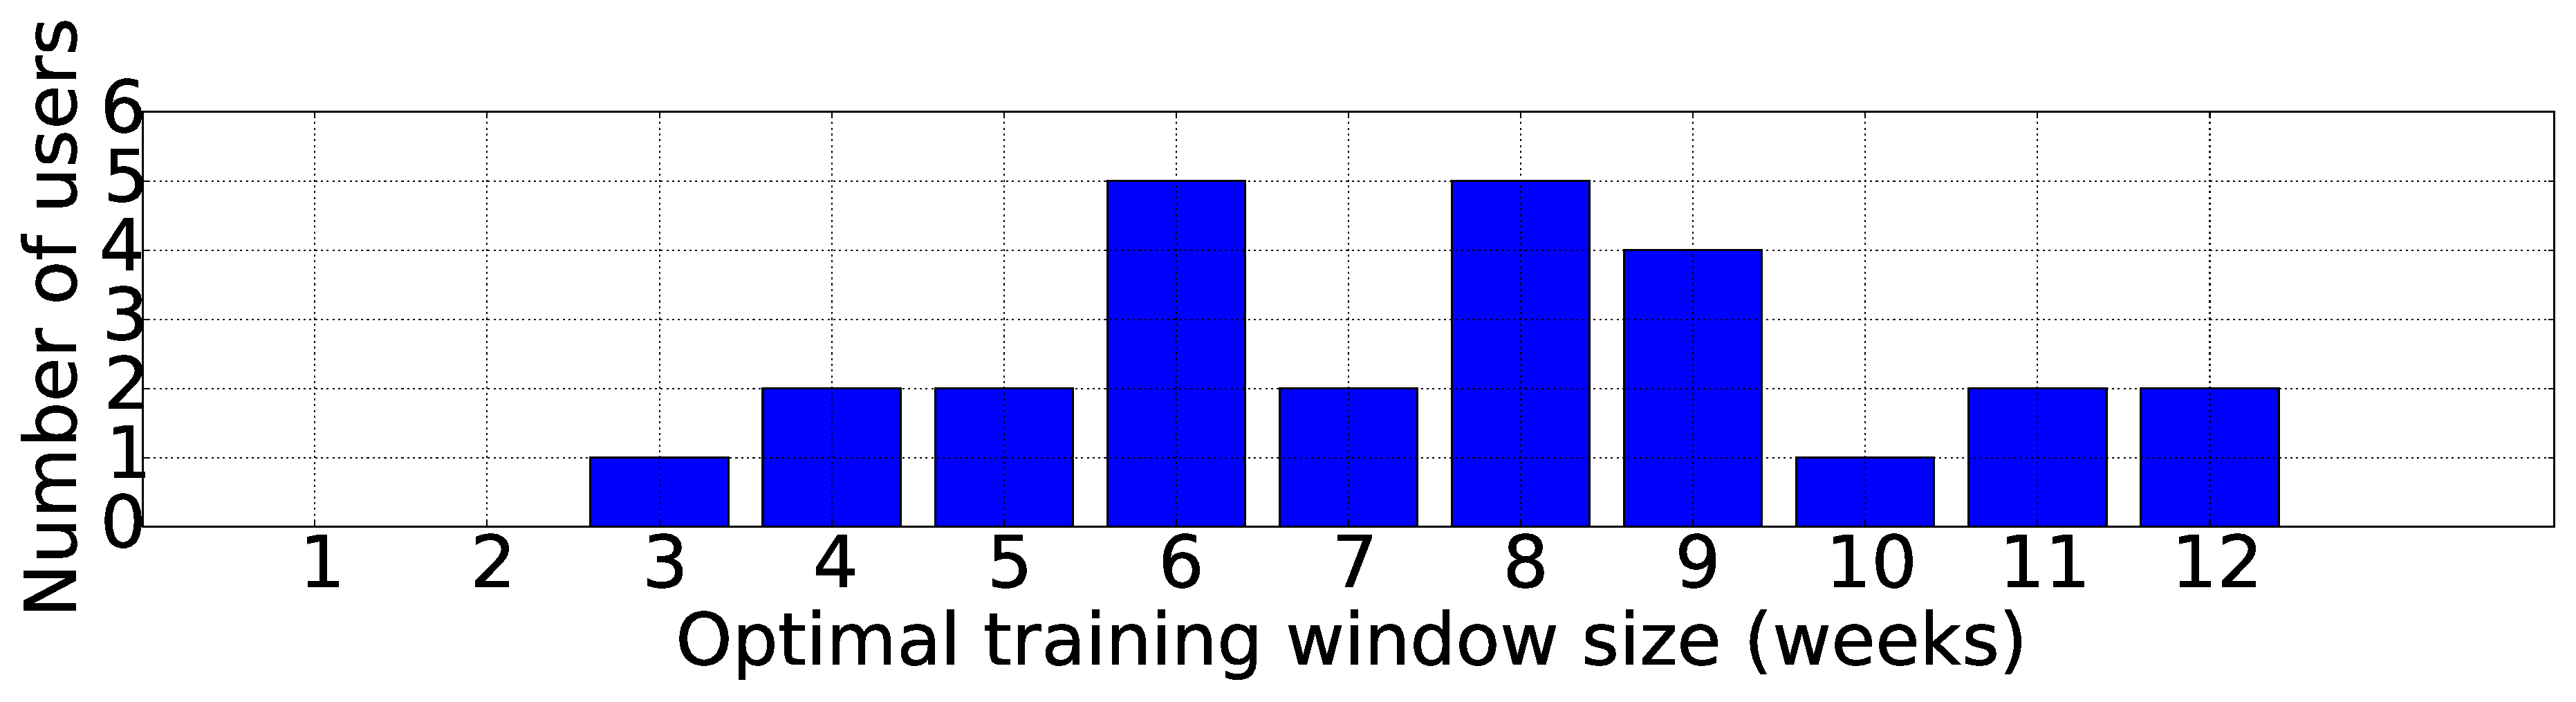
\includegraphics[width=0.95\linewidth]{FileAccess/figs/histogram_leastbestweekfscore6216New}
\caption{Distribution of the least number of weeks for each user of share D that gives highest F-score. } 
\label{fig:histBestLeastWeek6216}
\end{center}
%\vspace{-0.3in}
\end{figure}

Next, we perform a thorough study of the effect of training window
size on the performance of the models of individual users.  For this
purpose, we select share D, and divide its data into 17
parts, each corresponding to one week.  We remove 4 out of 30 users
because they do not have sufficient activity in each week.  We then
pick the last five weeks for the testing period, and create 12
different training windows, varying from 1 week to 12 weeks.  Based on
the results, we plot (Figure~\ref{fig:histBestLeastWeek6216}) the
distribution of the optimal training window size (in terms the least
number of weeks) providing the highest F-score for the evaluation
users of share D.  The median and the mode of this window is 8
weeks even though there are longer training windows up to 12 weeks,
thereby confirming our previous assertion that more training data does
not necessarily translate into better performance.  Additionally, we observe that
the optimal window size varies for each user.  The most active user
(with highest activity count) requires 4 weeks, whereas the least
active user requires 11 weeks.  This suggests that the optimal window
also depends on workload, with more active users requiring lesser
training time.

In a practical deployment, we could use an online evaluation approach
to continuously tune the system based on performance and workload
characteristics.  Lastly, it is important to note that some of the
recommended files, which are flagged as false positives in our
experiments, could in fact be true positives in an actual deployment
because users may genuinely find them useful.  Hence a precision
reported in this evaluation serves as the lower bound for the
precision expected from an actual deployment.


%% \indent We next study how the performance of the models of individual users varies for different training durations. In order to do so, we divide the data from share D on a weekly basis. Four out of 30 users do not have sufficient activity in each week and are hence removed in this analysis. For the same reason we have not provided these results for all eight shares. Figure~\ref{fig:histBestLeastWeek6216} shows the distribution of the least number of weeks that gives the highest F-score for evaluation users in share D. 
%% %\indent In order to analyze the performance variation of metadata models with finer time slices and on a per-user basis, 
%% %Only the training periods are varied 
%% For Figure~\ref{fig:histBestLeastWeek6216}, the test period comprises of the last five weeks to ensure that the 26 users have sufficient test data. 
%% The median and mode of the number of weeks giving highest F-score is seen to be 8 even though there are training periods that are 12 weeks long, showing that more training data need not improve the performance of a user model. It can be seen that the minimum size of training data required to give best F-score varies for each user. 
%% Due to space constraints, we are unable to provide complete statistics on activity rate of each user, and the performance variation of the user models. 
%% It is observed that while 4 weeks led to best performance for the most active user (in terms of the number of file activities in the share), the model corresponding to user with least activity required 11 weeks worth of training to provide best performance. This suggests that the optimal training duration differs for different users depending on their workloads. More active users typically need less number of weeks to collect sufficient activity to train a model that performs well. It is also seen that usually very small durations of training data do not lead to high performing models.

%% It must be mentioned that the entire performance evaluation of the system as described in this section is based on past activity. Upon actual deployment, the predictions can
%% be continuously compared with the actual accesses that users
%% make. This facilitates an online evaluation framework which can tune
%% the system parameters and adapt it based on the file edit rate, system performance and the
%% workload. For example using this framework, the size of training window and
%% frequency of re-training user models can be adjusted on a per-user basis to determine most
%% suitable values. In addition, as a result of the deployment of
%% the system, users would be able to discover files that they were
%% previously unaware of. It is possible that files that are considered
%% false positives by the evaluation framework presented in this paper, would be accessed
%% by users based on recommendations, and would hence be true positives
%% instead. Thus the precision reported in the current evaluation serves
%% as a lower bound for the precision expected upon actual deployment of
%% the system.
 
\subsection{Scalability}
\label{sec:scalability}
%%
Unlike training, which is an offline process, classification needs to
be performed in real time.  Therefore, we analyze time and space
complexities of only the testing, i.e., the classification phase.

\subsubsection{Time complexity}
In an actual deployment, whenever a file is created or modified in a
share, our system applies personalized models of each user in the
share.  Therefore, the runtime performance depends on the rate of file
edit operations $R_{edit}$ (in files per second) and the number of users $N$.

Let us compute the time taken to classify one file.  Let
$T_{meta\_model}$ and $T_{cf\_model}$ represent the average times (in seconds) 
required to apply a metadata model, and a CF model respectively.  We
need time $T_{meta\_feature}$ seconds to extract metadata features, and
$NT_{meta\_model}$ seconds to extract collaborative filtering features by
applying the metadata model of each user.  We then apply the CF model
of each user, which takes $NT_{cf\_model}$ seconds.  Thus, the total
classification time for one file is: $T_{meta\_feature} +
NT_{meta\_model} + NT_{cf\_model}$ seconds.


To make approximate calculations, we replace $T_{meta\_model}$ with
$T_{cf\_model}$ and ignore
$T_{meta\_feature}$ because it is negligible as compared to
$NT_{cf\_model}$.  Thus, it would take total time of
$2NT_{cf\_model}R_{edit}$ seconds to process all the files edited in each second.  Considering
the sample values we observed for some of the high workload shares: $N
= 16,000$, $R_{edit} = 5$ files/second, $T_{cf\_model} =
19\times10^{-3}$ second, the total time would be $3040$
seconds. Hence, in order to process all the files created or modified per 
second, we would need at least 48 64-core machines, with each core
concurrently performing classification.

Undoubtedly, the computational resources required to handle this kind
of workload would amount to a significant financial cost to the
enterprise.  In the next section, we address this problem by
presenting an optimization technique that substantially lowers the
computational requirements without sacrificing classification
accuracy.  With this improvement, we need just one 64-core machine to
manage the above mentioned heavy workload.

\subsubsection{Space complexity}
Unlike computation, memory requirements of our system are quite modest
even for heavy workloads.  Considering values: $N=16,000$, $R_{edit} =
5$ files/second, $F_{meta} = 35,000$ (highest number of metadata features in our
datasets), and $S$ = 4 bytes (size of value and weight of a feature),
we would need maximum ($F_{meta} + N) R_{edit} S$  i.e., nearly 1MB memory for all
the features in the worst case.  Note that the features of a file
remain the same for all the user models.  Each metadata model is
represented by $F_{meta}$ weights, and each CF model is represented by
$F_{meta} + N$ weights.  Thus, the total memory to store metadata and
CF models of all the users is: $(2F_{meta} + N) \times NS$ i.e., approximately 5 GB.  In
practice, the required memory would be much smaller because
collaborative filtering will be applied to a small subset of users
that show high degree of collaboration.

\comment {
\subsection{Scalability and Complexity Analysis}
\label{sec:scalability}

In the proposed system, the feature vector of each file is sparse and
is the same for all user models in a share. Let $N_{Meta}$ denote the number of metadata features and $N_{AM,f}$ denote the number of
metadata features of $f$ that are $active$, i.e., have a non-zero value. We use a sparse representation for the metadata features and as a result, the space requirement by a file $f$ when metadata models are used is only $O(N_{AM,f})$, which is typically much less than what it would have been if a sparse representation were not used, i.e., $O(N_{Meta})$. The space requirement of $f$ when CF models are used is $O(N_{AM,f} + \mid\!\!U\!\!\mid)$ since in addition to the active metadata features, features corresponding to predicted labels by
$\mid\!\!U\!\!\mid$ metadata models also need to be stored.

During testing, personalized models for each user in the share need to
be applied on every created or modified file. Let $R_{edit}$ denote
the rate of file generation or modification, in terms of files per
second. For using metadata models, the total time taken to process all files edited (i.e.,
created or modified) per second is equal to
\begin{equation} 
\label{eq:speedupmotv}
T_{Proc} = [ T_{Tok}  + T_{FeatEx} + \{ T_{Model} \times \mid\!\!U\!\!\mid \} ] \times R_{edit}. 
\end{equation}
$T_{Tok}$, $T_{FeatEx}$, $T_{Model}$ are the times in seconds to tokenize, extract features from, and apply a metadata model on a file respectively. \begin{math}T_{Tok}  + T_{FeatEx}\end{math} is typically negligible as compared to \begin{math} T_{Model}\times \mid\!\!U\!\!\mid  \end{math}. 
Thus the testing time complexity of our system varies as $O(\mid\!\!U\!\!\mid \times R_{edit})$. 
Note that during testing with CF models, $\mid\!\!U\!\!\mid$ metadata models need to be applied on each file, followed by $\mid\!\!U\!\!\mid$ CF models. Also, the time to apply CF models is at least as much as the time to apply metadata base models (i.e., $T_{Model}$) since the former models are based on more features. Thus $T_{Proc}$ for CF models is at least twice as much as that obtained using (\ref{eq:speedupmotv}). We provide numerical values below for metadata models. For CF models, the time taken would be approximately multiplied by a factor of two. 
%However for the below calculation, we only consider the $T_{Proc}$ for metadata models.
On a 2.7GHz 32GB machine, \begin{math}T_{Model}\end{math} for share G for the training set that gives highest F-score has a mean of 19 milliseconds and maximum of 60 milliseconds per file per user model, across 30 evaluation users. %, and is maximum 60 milliseconds. The high rate of content generation and modification in enterprises has been discussed in Section~\ref{sec:introduction}. 
%<!-- As a specific example, the average rate of file edits (file write or create operations) for Share I is 0.21 file edits per second. --> 
 By analyzing the recent file activity in several network file shares,
 we observe that \begin{math}R_{edit} \end{math} can be over 300 file
 edits per minute on average. We also observe that there are shares
 with activities from over 16,000 users,
 i.e., \begin{math}\mid\!\!U\!\!\mid\end{math} can be over 16,000.
   Using (\ref{eq:speedupmotv}), \begin{math} T_{Proc} \end{math} is equal to 1520
   seconds. This means that 
%4800 seconds 
% the number was 36 seconds earlier. This implies that on an average, more than four 8-core computers or more than one 32-core computer would be required to continuously process the edited content in one share. --> 
in order to provide recommendations for all edited files on a share, our system could require as many as 24 64-core machines on average. In addition to the high computational requirement on average, it is also observed that file edits often appear in bursts thereby leading to further increase in the load during peak hours. The high computational requirement associated with implementing the proposed system translates to a significant financial burden on the enterprise and may even render recommending content to users infeasible. In order to address these shortcomings, the next section proposes an approach that can substantially lower the computational requirement during testing. Based on the proposed approach, we show that the implementation of our system even for a large share can be done using the computational resources provided by just one 32 core machine. 
%and 75 machines when file edit rate is high. 
%75 64-core machines! 
%Such a high computational requirement in testing 
% Based on above, an enterprise having tens of thousands of shares may need a cluster having tens of thousands of powerful computers to determine which user may be interested in a new or modified content. This -->
%translates to significant financial burden on the enterprise which may even render recommending content to users infeasible. In addition, it is observed that file edits often appear in bursts and this may further increase the computational load during peak hours. 
%The figure below provides the distribution of the number of file edits (i.e., create or write) activities per minute that occur in share I. Among the minutes that saw any file edit activity, the mean number of file activities is 178, the 95-percentile is 450 and the maximum is 2889. In order to process 95\% of the active minutes, the proposed system needs to process at least 450 files per minute. That gives <math> T_{Process~All~Files~Edited~Per~Second} = 1282.05 </math> seconds. That is, due to bursty characteristic of file edits,  is, more than 160 8-core machines or 40 32-core machines would be required to process the content created or modified per second. -->
%It must be mentioned that the rate of content generation in enterprises increases by 40-50\% every year and this vastly overshadows the rate of growth in processor clock speeds or even in number of processors per machine [cite]. Thus the gap between rate of content generation and computational power will only increase in future and it is necessary to investigate approaches that can reduce the time it takes to recommend a new file to interested users. This is the motivation for developing a technique that can speed-up the testing process by several orders. 
%gracefully 
%As files are generated or modified on a share, our system needs to apply personalized model of each user to make the predictions. Therefore, We can address these factors to optimize the testing time as discussed in Section~{\ref{sec:futurework}}.  
}
\comment{
A significant obstacle for this system in terms of scalability
is the fact that each user has a personalized model.  Section~{\ref{sec:conclusion}} points out the potential to
reduce the testing time by selecting the user models to apply on a new
file. 
} 
\comment{
In terms of deployment, file recommendation is not necessarily
required for all users and file servers.  We can only enable the
recommendations on those file servers that aren't home shares or that
do not run applications that we are not interested in, such as backup,
or tasks run by administrators. For example, it would not make much
sense to deploy this system on a Linux style networked home directory.
It may not make much sense to provide file recommendation to
low-volume file users, but rather focus on enterprise search when they
do need to find information. It may be prudent to train a model for
only the users that are determined to be sufficiently active in a
share, constituting a small proportion of the total user
population. Further, training CF would not be recommended for
shares showing less degree of collaboration as evidenced by normalized
triangle counts.
Moreover, a recommendation system may
not be essential for all the file servers. For instance, it would not make 
much sense to deploy our system on a networked home directory or on a 
backup server. Additionally, it may 
not make much sense to provide file recommendation to low-volume file users, but 
rather focus on enterprise search when they do need to find information. 
It may be prudent to train a model for only the users that are determined to be 
sufficiently active in a share. 
%we can ignore home shares or backup servers.  Additionally, we don't need personalized
%models for users who are not active.  
Furthermore, for shares that do not demonstrate high degree of user collaboration, 
training and using CF models may not be recommended since they are computationally 
much more expensive than metadata models.
} 







\comment{
Updates (last day of intern): 
On-demand computing from Amazon EC2 shows that corresponding to 75 64-core machines, it would cost us: 
1.120*8*75*24*30*12 dollars per year = more than 5.8 million USD!  (for one large repository) 
The number 1.120 is for On-Demand can be changed to 0.4640 since latter is for Reserved Instances. 
}


\section{Active Features-based Model Selection (AFMS)}
\label{sec:testspeedup}
%
To speed up the classification time, our optimization technique AFMS
leverages properties of a soft-margin linear SVM model.  In this
model, the predicted label for a file $f$ is determined using the
score:
%
\vspace{-0.1in}
\begin{equation} 
\vspace{-0.1in}
\label{eq:linearsvmsum}
g(f) = w_0 + \sum_{j=1}^{F}{w_j*x_j}
\end{equation}
%
Here, $F$ is the number of features, $w_0$ is the intercept, $w_j$ 
is the $j^{th}$ feature weight in the model, and $x_j$ is the value of the $j^{th}$
feature of the file. The model predicts label $1$ if $g(f) \ge 0$,
and $0$ otherwise.  Given that our features have non-negative values,
without applying the model we can predict label $0$ when the following
conditions are met:
%
\begin{itemize}
  \renewcommand{\labelitemi}{$\bullet$}
  \item \textbf{condition 1}: The intercept is negative, i.e., $w_0 <
    0$, and
  \item \textbf{condition 2}: None of the weights of active (non-zero)
    features is positive.
\end{itemize}
%
Under these conditions, $g(f)$ is always negative, and hence the predicted label
is $0$.  Otherwise, we need to apply the model to obtain the
classification label, which could be 0 or 1.  The AFMS technique uses
this key intuition to save the cost of applying classification models.
Of course, its effectiveness depends on the number of times the
conditions are matched. Unsurprisingly, as our experiments show, this
happens quite often (refer Table~\ref{tab:SpeedupPotentialStats}):
%
\begin{itemize}
    \renewcommand{\labelitemi}{$\bullet$}
\item \textbf{condition 1}: Around $96\%$ of the metadata models have negative
  intercept (i.e., $w_0 < 0$).  This is because a typical user
  accesses only a small fraction of files.  Owing to this natural
  imbalance, the model favors $0$ as the prediction label, resulting
  in a negative intercept.
\item \textbf{condition 2}: Our data shows sparsity of features
  with an average of only $2.2\%$ of metadata features being active (i.e., $x_j > 0$) in the files.
  Also, the average ratio of the features with positive weights (i.e., $w_j > 0$) per model is only
  $6.4\%$, and each of these features on an average has a positive weight in less
  than $10\%$ of the models.  The combination of these three facts
  significantly lowers the probability of finding active features with positive
  weights.
\end{itemize}
\begin{table*}
{\fontsize{8pt}{1em}\selectfont
\begin{center}
%\begin{tabular}{|>{\centering}p{0.065\linewidth}|>{\centering}p{0.2\linewidth}|>{\centering}p{0.25\linewidth}|>{\centering}p{0.2\linewidth}|>{\centering}p{0.23\linewidth}|}
%  \hline
\caption{ Statistics for metadata models, averaged across 30 evaluation users and
  different training periods (Section~\ref{sec:varytraintest}), showing how
  AFMS is effective.}
\begin{tabular}{|c|r|r|r|r|}
  \hline

\textbf{Share} & \textbf{\% models with} & \textbf{\% active} &
\textbf{\% features with} & \textbf{\% models per} \tabularnewline
& \textbf{negative intercept} & \textbf{features} & \textbf{positive
weight} & \textbf{positive feature} \tabularnewline \hline

A & 100.0 & 0.10 & 2.8 & 2.8  \tabularnewline  \hline
B & 98.9 & 1.90 & 2.5 & 3.6   \tabularnewline  \hline
C & 100.0 & 0.10 & 0.2 & 0.2  \tabularnewline  \hline
D & 100.0 & 6.60 & 0.8 & 0.8  \tabularnewline  \hline
E & 96.1 & 1.40 & 15.2 & 18.5 \tabularnewline  \hline
F & 98.3 & 1.60 & 4.2 & 5.8   \tabularnewline  \hline
G & 74.5 & 6.10 & 21.7 & 40.8 \tabularnewline  \hline
H & 100.0 & 0.01 & 4.1 & 4.1  \tabularnewline  \hline
\textbf{Avg.} & \textbf{95.9} & \textbf{2.2} & \textbf{6.4} & \textbf{9.6} \tabularnewline \hline
\end{tabular}
\end{center}
}
\vspace{-0.1in}

\label{tab:SpeedupPotentialStats}
\end{table*}
The favorable statistics result in matching the conditions quite
often, thereby leading to faster testing of files because the cost of
checking the conditions is negligible. Note that faster testing of files is 
referred to as better performance in the discussion below. 
While we have provided the above 
statistics based on the metadata models, similar trends are observed for CF models 
as well. 
Section~\ref{sec:exptspeedup}
shows the actual gains in the performance for both metadata and CF models.  The next section describes
the algorithm to implement AFMS.

\subsection{AFMS Algorithm}
\label{sec:AFMSAlgorithm}

\begin{algorithm*}[t!]
  \fontsize{8pt}{1em}\selectfont
  \caption{AFMS Classification}
  \label{algo:AFMSClassification}
  \vspace{0.3cm}
  \textbf{Variables definitions}:

  \begin{itemize}
      \renewcommand{\labelitemi}{}
    \NumTabs{10}
  \item $N$ \tab: Number of users
  \item $F_{meta}$ \tab: Number of metadata features
  \item $F_{CF}$ \tab: Number of features in CF models = $F_{meta} + N$
  \item $w_{\sigma(i, j)}$\tab: Weight of $j^{th}$ feature in $i^{th}$ user
  model, $1 \le i \le N$, $1 \le j \le F_\sigma$, $\sigma \in \{meta,
    CF\}$
  \end{itemize}

  \textbf{Offline pre-processing to be done right after model training}:\\

  \quad $FTM_{\sigma}(j) = \{ i \mid w_{\sigma(i, j)} \ge \tau$, or
      $w_{\sigma(i, 0)} > 0 \}$\\

  \textbf{Classification}:\\

  \quad \textbf{Input}:
  
  \quad\quad $X = [x_1, x_2, \dots, x_{F_{meta}}]\>$ :  Metadata feature
  vector of the test file $f$\\
  
  \quad \textbf{Output}:
  
  \quad\quad $Y = [y_1, y_2, \dots, y_N]$ \qquad  : Predicted classification label ($0$ or $1$) by metadata models for each user \\ 

  \quad\quad $L = [l_1, l_2, \dots, l_N]$ \qquad\quad : Predicted classification label ($0$ or $1$) by CF models for
  each user\\
  
  \quad \textbf{Procedure}:\\

  \quad\quad $M = C = \{\}$ \qquad\qquad \thinspace\thinspace\thinspace\thinspace\thinspace \codecomment initialize
  triggered metadata and CF models
  
  \quad\quad \keyword{for} $i$ = $1$ \keyword{to} $N$:
  \qquad\quad\enspace\thinspace\thinspace\thinspace \thinspace\codecomment initialize CF features and output labels

  \quad\quad\qquad $Y[i] = L[i] = 0$\\

  
  \quad\quad \keyword{for} $j$ = $1$ \keyword{to} $F_{meta}$:
  \qquad \codecomment step1: obtain triggered metadata models

  \quad\quad\qquad \keyword{if} ($X[j]$):
  
  \quad\quad\qquad\qquad $M = M \cup FTM_{meta}(j)$\\

  \quad\quad \keyword{for} $i$ \keyword{in} $M$: \qquad\qquad\quad\thinspace$\,$
  \codecomment step2: compute CF features
  
  \quad\quad\qquad $Y[i]$ = ApplyMetadataModel($i$, $X$)\\
  
  \quad\quad $X = [X, Y]$ \qquad\qquad \thinspace\thinspace\thinspace\thinspace\thinspace\thinspace\thinspace\thinspace \codecomment step3: append CF features to
  metadata features\\

  \quad\quad \keyword{for} $j$ = $1$ \keyword{to} $F_{CF}$:
  \qquad\thinspace$\>$ \codecomment step4: obtain triggered CF models

  \quad\quad\qquad \keyword{if} ($X[j]$):

  \quad\quad\qquad\qquad $C = C \cup FTM_{CF}(j)$\\  
  
  \quad\quad \keyword{for} $i$ \keyword{in} $C$: \qquad\qquad\quad\enspace\enspace
  \codecomment step5: compute CF model labels
  
  \quad\quad\qquad$L[i]$ = ApplyCFModel($i$, $X$)\\
  
\end{algorithm*}


\begin{figure}[htp]
\centering
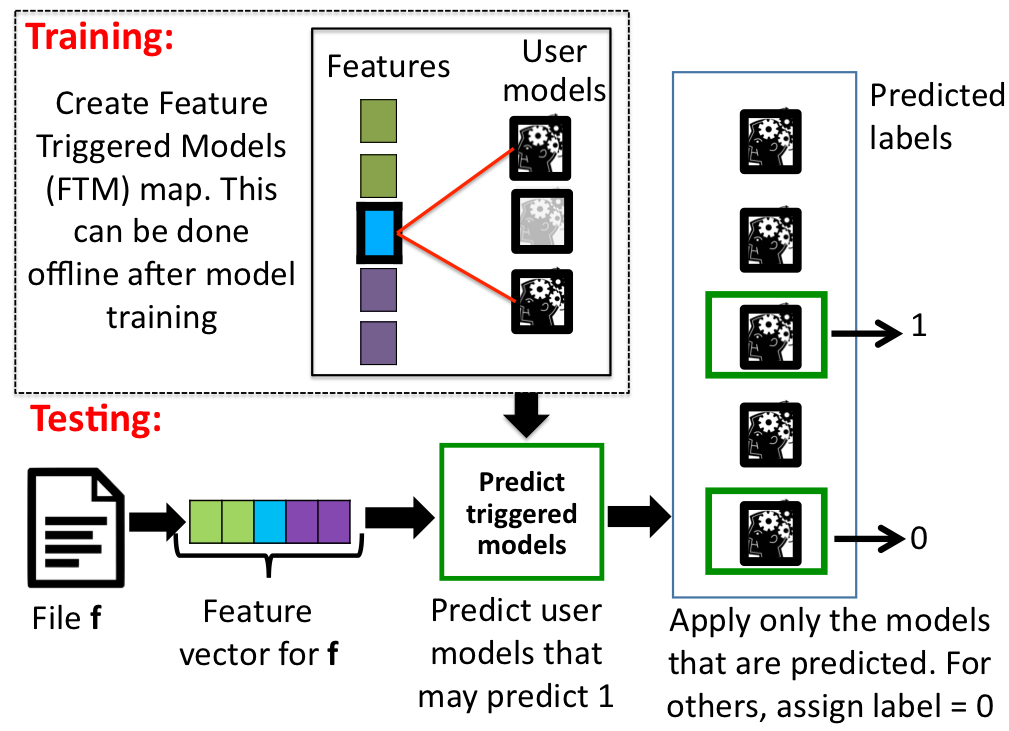
\includegraphics[width=0.75\linewidth]{FileAccess/figs/framework_withspeedup.png} 
\caption{AFMS technique first creates FTM in an offline manner.  The
  classification step applies only those models that are triggered by
  active features.}
\label{fig:speedupframework}
\end{figure}
Our technique extends the basic idea to make the optimization tunable
so that it can potentially trade-off model correctness for even better classification
efficiency.  In order to do so, we
define that {\it a feature with index $j$ triggers a model} when $w_j
\ge \tau$ or $w_0 \ge 0$ where $w_0$ and $w_j$ are the intercept and the $j^{th}$ feature weight of the model respectively. Here, we use the threshold parameter $\tau
\ge 0$ to make the technique tunable. Given a test file, a model would be applied on it 
if any of the active features of the test file \textit{trigger} the model. 
For $\tau = 0$, there is no
loss of predictive correctness, and yet there is performance gain due to the
optimization.  However, as $\tau$ increases, fewer models are
triggered, and hence there is further improvement in the performance,
albeit at the cost of predictive correctness.  With fewer models being applied,
there will be more number of 0 as the predicted labels, and hence the
recall is expected to degrade.  However, precision and likewise
F-score can degrade or improve depending on the correctness of the recommendations.
Section~\ref{sec:exptspeedup} shows that we can gain significant
efficiency at marginal cost of model correctness.  Furthermore, the technique
can be made adaptive by varying $\tau$ based on the rate of file edit
operations at a given time.

Please refer to Algorithm~\ref{algo:AFMSClassification} to understand
variable definitions, and the details of the algorithm.  As part of
pre-processing, which is done right after the training phase, for each
feature we compute the set $FTM$ (Feature Triggered Models) consisting
of models that are triggered by the feature (Figure~\ref{fig:speedupframework}).  The algorithm computes
separate sets for metadata and CF models.

The input to the classification procedure is the array $X[1 \dots
  F_{meta}]$ of metadata features corresponding to the test 
file.  The procedure produces the outputs: an array $L[1 \dots N]$
consisting of prediction label for each of the $N$ users by CF models, and an array $Y[1 \dots N]$
consisting of prediction label by metadata models.  The
procedure initializes the output arrays with $0$ values as the default labels.  It also
initializes sets $M$ and $C$ that are later used to collect triggered
metadata and CF models respectively.  The first step obtains the set
of metadata models that are triggered by the active features. The
second step applies these metadata models to compute metadata predicted labels, which are also the CF features $Y$.  The third step appends the CF features to the metadata features. 
The fourth step obtains the set of CF models that are triggered by the
active features.  Finally, the last step applies these CF models to
compute the CF predicted labels.

If a model is not applied, the default label $0$ becomes the
predicted label, and the algorithm assigns a random negative value as
the confidence score for the label.  We need the confidence score
because it is used to determine the relative ranking of test files,
which is then used in the computation of recall at 75\%.  As a side
effect, it is possible that AR@75P for AFMS with $\tau = 0$ may differ
from AR@75P computed without AFMS.


\subsubsection{Complexity analysis}  In AFMS classification procedure,
steps 2 and 5 are the most expensive ones, requiring $O(N)$
classifications.  Thus, with the rate of file edit operation
$R_{edit}$, the algorithm needs to perform $O(NR_{edit})$
classifications.  The optimization does not change the worst case time
complexity because it is possible that all the models are triggered
for a particular dataset. However, given the presence of natural
class imbalance in user-activity datasets, our optimization
significantly improves the average case time complexity.  For
instance, with $\tau = 0.5$, testing of a single file on an average
requires approximately 0.5 metadata- and 0.2 CF-based classifications out of 30
evaluation users.  This reduces the classification time of metadata
and CF models by 62 and 169 times respectively. The next section
provides detailed performance results.

%% FIXME: Why don't these numbers match the numbers in the  result
%% section 

\subsection{AFMS Evaluation}
\label{sec:exptspeedup}
%%
We measure the performance improvement using a simple metric:
%%
\begin{equation}
\label{eq:speedupgain} 
\mbox{{\it Speed-up}} = \frac{\mbox{\# models applied without AFMS}}{\mbox{\# models applied with AFMS}}.
\end{equation}
%%
Speed-up provides a direct estimate of reduction in classification
time.


\begin{figure*}
\begin{minipage}{.95\textwidth}
\centering
\epsfig{width=0.65\linewidth,figure=FileAccess/figs/gains_thresh.eps}

\captionof{figure}{Speed-up vs. $\tau$ for metadata models}
\label{fig:gainvsThreshMeta}
\end{minipage}
\begin{minipage}{.95\textwidth}
\centering
\epsfig{width=0.65\linewidth,figure=FileAccess/figs/gains_with_threshCF.eps}

\captionof{figure}{Speed-up vs. $\tau$ for CF models} 
\label{fig:gainvsThreshCF}
\end{minipage}

\end{figure*}


Figures \ref{fig:gainvsThreshMeta}-\ref{fig:r75pvsThreshCF} show the
effect of $\tau$ on speed-up, and various correctness metrics including
average precision, recall, and F-score.  The numbers are averaged across all
the evaluation users, and all training and testing periods for
individual shares.

In general, we observe that speed-up increases exponentially with
respect to $\tau$, whereas the correctness metrics degrade almost linearly,
with a mild slope, as $\tau$ increases.  This clearly shows that AFMS
can obtain significant efficiency at marginal cost of accuracy.

%%
%% FIXME: Average AF (average of average) there is no cosistency in
%% in description and graphs
%%
%% Change Y axis labels for speedup graphs (fig 10, 11): Avg speedup
%% change ``speed-up'' -> ``speedup'' consistently everywhere
%%


As expected, for $\tau = 0$, AFMS does not lose accuracy, e.g., CF
model Avg AF values from Table~\ref{tab:CollabFilteringPerf} and
Figure~\ref{fig:fscorevsThreshCF} remain the same for all shares.  And
yet, AFMS provides 4 times average speed-up across all shares for metadata models, and 
6 times average speed-up for CF models. The speed-up for $\tau = 0$ is as high as 15 times and 23 times for share A for metadata and CF models respectively. 
With $\tau = 0.5$, the average speed-up for metadata models is 62 times, and for CF models is 169 times. The most gain is observed for share A as 147 times for metadata models, and 280 times for CF models. However, this
threshold affects the correctness, dropping averages across shares. For example, for CF models, the Avg AF changed 
from 49.6\% to 45.8\%, Avg AR from 48\% to 33.3\%, Avg AR@75P from 44.8\% to 36.9\%, but
slightly improving Avg AP from 38.9\% to 42.5\%.  These results
confirm the expected effect as discussed in
Section~\ref{sec:AFMSAlgorithm}.

\comment {
Figures~\ref{fig:gainvsThreshMeta} though \ref{fig:gainvsThreshCF} show
that speed-up increases exponentially with respect to $\tau$.  In
addition, Figures~\ref{fig:precisionvsThreshMeta} through
\ref{fig:r75pvsThreshMeta} show how the precision, recall, F-score,
and Recall@75\%Precision vary with $\tau$ for metadata models on
different shares. The numbers provided are averaged across evaluation
users and across all training and testing periods.
%Figure~\ref{fig:gainvsThreshMeta} shows the variation of the speed-up averaged across all test files, evaluation users and training and testing periods. 
As expected, AFMS with $\tau=0$ leads to the same F-score as without AFMS. Despite the same predictive correctness, AFMS speeds up the testing per file by 4 times on average across all shares, and by as high as 15 times for Share A. 
%(Share A). 
For $\tau=0.5$, the average speed-up across the evaluation shares is around 62 times, and is 147 times for Share A. For the same $\tau$, average F-score drops from 47\% to 43\%, average recall drops from 47\% to 37\% and average precision drops from 35\% to 34\%. Confirming to the discussion in Section~\ref{sec:AFMSdetails}, a higher $\tau$ leads to most loss in recall. 

Figures~\ref{fig:precisionvsThreshCF} through \ref{fig:r75pvsThreshCF} show the variation of the model performance metrics with $\tau$ for CF models. 
For our experiments, we have chosen the value of $\tau$ to be the same for Metadata-FTM and CF-FTM. %Also, for the calculation of speed-up for CF models as per Eq.~\ref{eq:speedupgain}, the metadata and the CF models have been considered equivalent. 
For CF models, $\tau=0$ leads to average speed-up of more than 6 times and $\tau=0.5$ leads to average speed-up of 170 times. The speed-up observed for Share A for $\tau=0.5$ is 280 times. The observed testing speed-up demonstrates that the proposed AFMS approach can significantly reduce the testing computational requirement of the proposed file recommendation system. 
\vspace{-0.2in}
}
% Metadata models 
\begin{figure*}[htb!]
\begin{minipage}{.95\textwidth}
\centering
\epsfig{width=0.65\linewidth,figure=FileAccess/figs/precisions_thresh.eps}
%\vspace{-0.15in}
\captionof{figure}{Precision vs. $\tau$ for metadata models}
\label{fig:precisionvsThreshMeta}
\end{minipage}
\begin{minipage}{.95\textwidth}
\centering
\epsfig{width=0.65\linewidth,figure=FileAccess/figs/recalls_thresh.eps}
%\vspace{-0.15in}
\captionof{figure}{Recall vs. $\tau$ for metadata models} 
\label{fig:recallvsThreshMeta}
\end{minipage}
\begin{minipage}{.95\textwidth}
\centering
\epsfig{width=0.65\linewidth,figure=FileAccess/figs/fscore_thresh.eps}
%\vspace{-0.15in}
\captionof{figure}{F-score vs. $\tau$ for metadata models}
\label{fig:fscorevsThreshMeta}
\end{minipage}
\begin{minipage}{.95\textwidth}
\centering
\epsfig{width=0.65\linewidth,figure=FileAccess/figs/r75p_thresh.eps}
%\vspace{-0.15in}
\captionof{figure}{Recall@75\%Precision vs. $\tau$ for metadata models} 
\label{fig:r75pvsThreshMeta}
\end{minipage}
%\vspace{-0.4in}
\end{figure*}


% CF models variations with threshold: 
\begin{figure*}[htb!]
\begin{minipage}{.95\textwidth}
\centering
\epsfig{width=0.65\linewidth,figure=FileAccess/figs/precision_with_threshCF.eps}
%\vspace{-0.1in}
\captionof{figure}{Precision vs. $\tau$ for CF models}
\label{fig:precisionvsThreshCF}
\end{minipage} 
\begin{minipage}{.95\textwidth}
\centering
\epsfig{width=0.65\linewidth,figure=FileAccess/figs/recalls_with_threshCF.eps}
%\vspace{-0.1in}
\captionof{figure}{Recall vs. $\tau$ for CF models} 
\label{fig:recallvsThreshCF}
\end{minipage} 
\begin{minipage}{.95\textwidth}
\centering
\epsfig{width=0.65\linewidth,figure=FileAccess/figs/fscores_with_threshCF.eps}
%\vspace{-0.1in}
\captionof{figure}{F-score vs. $\tau$ for CF models}
\label{fig:fscorevsThreshCF}
\end{minipage} 
\begin{minipage}{.95\textwidth}
\centering
\epsfig{width=0.65\linewidth,figure=FileAccess/figs/r75p_with_threshCF.eps}
%\vspace{-0.1in}
\captionof{figure}{Recall@75\%Precision vs. $\tau$ for CF models} 
\label{fig:r75pvsThreshCF}
\end{minipage} 
\end{figure*}

\comment{
\begin{figure}
\epsfig{width=0.95\linewidth,figure=FileAccess/figs/gains_with_threshCF.eps}
\caption{Variation of average speed-up gain with $\tau$ for CF models}
\label{fig:gainvsThreshCF}
\end{figure} 
}
\comment {
\begin{figure}
\centering
\epsfig{width=0.45\linewidth,figure=FileAccess/figs/gains_vs_fscoresCF.eps}
%\vspace{-0.15in}
\caption{Variation of average speed-up gain with AF for CF models. \CV{is this figure needed?}} 
\label{fig:gainvsfscoreCF}
\end{figure}
}

\comment{
\vspace{-0.2in}
\section{Experimental validation of AFMS }
\label{sec:exptspeedup}
We measure the reduction in the testing computational requirement of a file $f$ using \textit{speed-up} defined as follows: 
\begin{equation}
\label{eq:speedupgain} 
\mbox{speed-up} = \frac{\mbox{\# models applied on $f$ without AFMS}}{\mbox{\# models applied on $f$ with AFMS}}.
\end{equation}
%\CV{speedup seemed more attention grabbing than complexity. Let me know if this fits well }
\vspace{-0.2in}
\begin{figure*}
\begin{minipage}{.49\textwidth}
\epsfig{width=\linewidth,figure=FileAccess/figs/gains_thresh.eps}
\vspace{-0.15in}
\captionof{figure}{Variation of average speed-up gain with $\tau$ for metadata models}
\label{fig:gainvsThreshMeta}
\end{minipage}
\begin{minipage}{.49\textwidth}
\epsfig{width=\linewidth,figure=FileAccess/figs/gains_with_threshCF.eps}
\vspace{-0.15in}
\captionof{figure}{Variation of average speed-up gain with $\tau$ for CF models} 
\label{fig:gainvsThreshCF}
\end{minipage}
\vspace{-0.15in}
\end{figure*}

Figures~\ref{fig:gainvsThreshMeta} and \ref{fig:gainvsThreshCF} show how the speed-up varies with $\tau$ for different shares for Metadata and CF models respectively. In addition, Figures~\ref{fig:precisionvsThreshMeta} through \ref{fig:r75pvsThreshMeta} show how the precision, recall, F-score, and Recall@75\%Precision vary with $\tau$ for metadata models on different shares. The numbers provided are averaged across evaluation users and across all training and testing periods. 
%Figure~\ref{fig:gainvsThreshMeta} shows the variation of the speed-up averaged across all test files, evaluation users and training and testing periods. 
As expected, AFMS with $\tau=0$ leads to the same F-score as without AFMS. Despite the same predictive correctness, AFMS speeds up the testing per file by 4 times on average across all shares, and by as high as 15 times for Share A. 
%(Share A). 
For $\tau=0.5$, the average speed-up across the evaluation shares is around 62 times, and is 147 times for Share A. For the same $\tau$, average F-score drops from 47\% to 43\%, average recall drops from 47\% to 37\% and average precision drops from 35\% to 34\%. Confirming to the discussion in Section~\ref{sec:AFMSdetails}, a higher $\tau$ leads to most loss in recall. 

Figures~\ref{fig:precisionvsThreshCF} through \ref{fig:r75pvsThreshCF} show the variation of the model performance metrics with $\tau$ for CF models. 
For our experiments, we have chosen the value of $\tau$ to be the same for Metadata-FTM and CF-FTM. %Also, for the calculation of speed-up for CF models as per Eq.~\ref{eq:speedupgain}, the metadata and the CF models have been considered equivalent. 
For CF models, $\tau=0$ leads to average speed-up of more than 6 times and $\tau=0.5$ leads to average speed-up of 170 times. The speed-up observed for Share A for $\tau=0.5$ is 280 times. The observed testing speed-up demonstrates that the proposed AFMS approach can significantly reduce the testing computational requirement of the proposed file recommendation system. 
\vspace{-0.2in}
% Metadata models 
\begin{figure*}[htb!]
\begin{minipage}{.49\textwidth}
\epsfig{width=0.85\linewidth,figure=FileAccess/figs/precisions_thresh.eps}
\vspace{-0.15in}
\captionof{figure}{Variation of the average precision (AP) with $\tau$ for metadata models}
\label{fig:precisionvsThreshMeta}
\end{minipage}
\begin{minipage}{.49\textwidth}
\epsfig{width=0.85\linewidth,figure=FileAccess/figs/recalls_thresh.eps}
\vspace{-0.15in}
\captionof{figure}{Variation of the average recall (AR) with $\tau$ for metadata models} 
\label{fig:recallvsThreshMeta}
\end{minipage}
\begin{minipage}{.49\textwidth}
\epsfig{width=0.85\linewidth,figure=FileAccess/figs/fscore_thresh.eps}
\vspace{-0.15in}
\captionof{figure}{Variation of the average F-score (AF) with $\tau$ for metadata models}
\label{fig:fscorevsThreshMeta}
\end{minipage}
\begin{minipage}{.49\textwidth}
\epsfig{width=0.85\linewidth,figure=FileAccess/figs/r75p_thresh.eps}
\vspace{-0.15in}
\captionof{figure}{Variation of the average recall at 75\% P (AR@75P) with $\tau$ for metadata models} 
\label{fig:r75pvsThreshMeta}
\end{minipage}
\vspace{-0.4in}
\end{figure*}

\begin{figure}[!htb]
\centering
\epsfig{width=0.45\linewidth,figure=FileAccess/figs/gains_vs_fscore.eps}
\vspace{-0.1in}
\caption{Variation of average speed-up gain with AF for metadata models \CV{is this figure needed?}} 
\label{fig:gainvsfscoreMeta}
\end{figure}

% CF models variations with threshold: 
\begin{figure*}[htb!]
\begin{minipage}{.49\textwidth}
\epsfig{width=\linewidth,figure=FileAccess/figs/precision_with_threshCF.eps}
\vspace{-0.1in}
\captionof{figure}{Variation of average precision (AP) with $\tau$ for CF models}
\label{fig:precisionvsThreshCF}
\end{minipage} 
\begin{minipage}{.49\textwidth}
\epsfig{width=\linewidth,figure=FileAccess/figs/recalls_with_threshCF.eps}
\vspace{-0.1in}
\captionof{figure}{Variation of average recall (AR) with $\tau$ for CF models} 
\label{fig:recallvsThreshCF}
\end{minipage} 
\begin{minipage}{.49\textwidth}
\epsfig{width=\linewidth,figure=FileAccess/figs/fscores_with_threshCF.eps}
\vspace{-0.1in}
\captionof{figure}{Variation of average F-score (AF) with $\tau$ for CF models}
\label{fig:fscorevsThreshCF}
\end{minipage} 
\begin{minipage}{.49\textwidth}
\epsfig{width=\linewidth,figure=FileAccess/figs/r75p_with_threshCF.eps}
\vspace{-0.1in}
\captionof{figure}{Variation of average recall at 75\% precision (AR@75P) with $\tau$ for CF models} 
\label{fig:r75pvsThreshCF}
\end{minipage} 
\end{figure*}

\begin{figure}
\centering
\epsfig{width=0.45\linewidth,figure=FileAccess/figs/gains_vs_fscoresCF.eps}
\vspace{-0.15in}
\caption{Variation of average speed-up gain with AF for CF models. \CV{is this figure needed?}} 
\label{fig:gainvsfscoreCF}
\end{figure}
}



%
%% In order to explain the proposed Active Feature based Model
%% Selection (AFMS) approach, we first provide an observation regarding linear
%% SVMs that have been used to model user access patterns in our system,
%% followed by insights learnt from actual data and trained models. We then provide details on how AFMS can be used to reduce the testing computational requirement. 

%% \textbf{Observations on linear SVM.} Given a linear SVM model $M$, the
%% predicted label for a file $f$ is calculated based on the score $M(f)$
%% where
%% \vspace{-0.1in}
%% \begin{equation} 
%% \vspace{-0.1in}
%% \label{eq:linearsvmsum}
%% M(f) = w_{0,M} + \sum_{j=1}^{N}{w_{j,M}*f_j}. 
%% \end{equation} 
%% Here, $w_{0,M} \in \mathbb{R}$ is the intercept and $w_{j,M} \in \mathbb{R}$ $\forall j \in [1,N]$ are the learnt feature weights of the trained model $M$. $f_j$ is the value of the $j^{th}$ feature of $f$ and $N$ is the number of features. The model predicts label 1 if $M(f) > 0$, and 0 otherwise. Thus if $w_{0,M}<0$, then a necessary condition for $M$ to predict 1 for file $f$ is that $f$ has at least one such feature that $M$ has positive feature weight for. Based on the above, and the fact that the defined features in Section~\ref{sec:features} are either positive or zero, the following can be concluded: The set of models that have positive feature weight for at least one of the non-zero features of a test file $f$ is a superset of the set of models that would predict label 1 for $f$. Thus given a test file $f$, it can be said that the models that do not have positive features for any of the non-zero features of $f$ would predict label 0 and need not be applied on $f$. This is the key intuition behind the proposed AFMS approach. 
%% \begin{table}
%% {\fontsize{8pt}{1em}\selectfont
%% \begin{center}
%% \begin{tabular}{|>{\centering}p{0.065\linewidth}|>{\centering}p{0.2\linewidth}|>{\centering}p{0.25\linewidth}|>{\centering}p{0.2\linewidth}|>{\centering}p{0.23\linewidth}|} \hline
%% \textbf{Share} &  \textbf{\% non-zero features} & \textbf{\% models with non-negative intercept (out of 30)} & \textbf{\% features with positive weights in models} & \textbf{\% triggered models per feature (out of 30)} \tabularnewline  \hline
%% A & 0.1 & 0.0 & 2.8 & 2.8    \tabularnewline  \hline
%% B & 1.9 & 1.1 & 2.5 & 3.6   \tabularnewline  \hline
%% C & 0.1 & 0.0 & 0.2 & 0.2  \tabularnewline  \hline
%% D & 6.6 & 0.0 & 0.8 & 0.8   \tabularnewline  \hline
%% E & 1.4 & 3.9 & 15.2 & 18.5  \tabularnewline  \hline
%% F & 1.6 & 1.7 & 4.2 & 5.8  \tabularnewline  \hline
%% G & 6.1 & 25.5 & 21.7 & 40.8  \tabularnewline  \hline
%% H & 0.01 & 0.0 & 4.1 & 4.1  \tabularnewline  \hline
%% \end{tabular}
%% \end{center}
%% }
%% \vspace{-0.1in}
%% \caption{Analysis of feature sparsity and of trained metadata based user models per share. The model statistics are averaged across 30 evaluation users and different training periods as described in Section~\ref{sec:varytraintest}. }
%% \label{tab:SpeedupPotentialStats}
%% \end{table}

%% \textbf{Insights from data and trained models.}
%% We provide below insights regarding the feature sparsity of enterprise data, and relate class bias in the trained user models with individual features. 
%% %\indent In addition to making the above observation about linear SVMs, we analyze the trained metadata user models for insights relating to the bias in the models, and the relationship between models and individual features. These are summarized below. 
%% \begin{itemize}
%% \item The features used in our system demonstrate significant sparsity. Table~\ref{tab:SpeedupPotentialStats} shows that only 0.01\% to 6.1\% of the metadata features are non zero. For CF models, it is observed that on average across all shares, only 2.1\% of the features are non zero. 
%% \item The training data for most user models has a high amount of
%%   class imbalance, favoring class 0. This is because for a typical
%%   user, most of the files observed in training period are not accessed by the user. As a result, the trained linear SVM models
%%   typically have a negative intercept (i.e., $w_{0,M} < 0$ in
%%   Eq.~\ref{eq:linearsvmsum}), suggesting the classifier has an a
%%   priori expectation of the user not accessing the file.
%% %, followed by negative or positive feature weights.
%% Table~\ref{tab:SpeedupPotentialStats} shows that for half of the eight
%% evaluation shares, all the trained metadata models have negative
%% intercepts, and that across all eight shares, only 4\% of models have
%% non-negative intercepts.
%% \item The trained models typically have positive feature weight (i.e.,
%%   $w_{j,M} > 0$ in Eq.~\ref{eq:linearsvmsum}) for only few features. Table~\ref{tab:SpeedupPotentialStats} shows that on
%%   average, the fraction of features having positive weight in trained
%%   metadata models with negative intercept is only 6.4\%.
%% \item Table~\ref{tab:SpeedupPotentialStats} also shows that each
%%   feature on average has positive weights in less than 10\% of models
%%   in a share.
%% %. On an average, the models have a positive weight for only 6.4\% of the features. 
%% %\item Among the models that have negative intercept, only XX\% of the features on an average have positive weight 
%% \end{itemize} 
%% The above insights suggest that through selecting the user models to apply on a test file, using its non zero features, it may be possible to achieve significant reduction in the testing complexity without substantial loss in model correctness. Section~\ref{sec:exptspeedup} validates our hypothesis through experiments. We provide details of the proposed approach (AFMS) below and also show how AFMS can, in addition, trade-off model correctness for further lowering of the testing complexity.
%% %This is the basis of AFMS based approach to speed-up the testing per file. 

\comment {
\subsection{AFMS Implementation}
\label{sec:AFMSdetails}
\begin{figure}[htp]
\centering
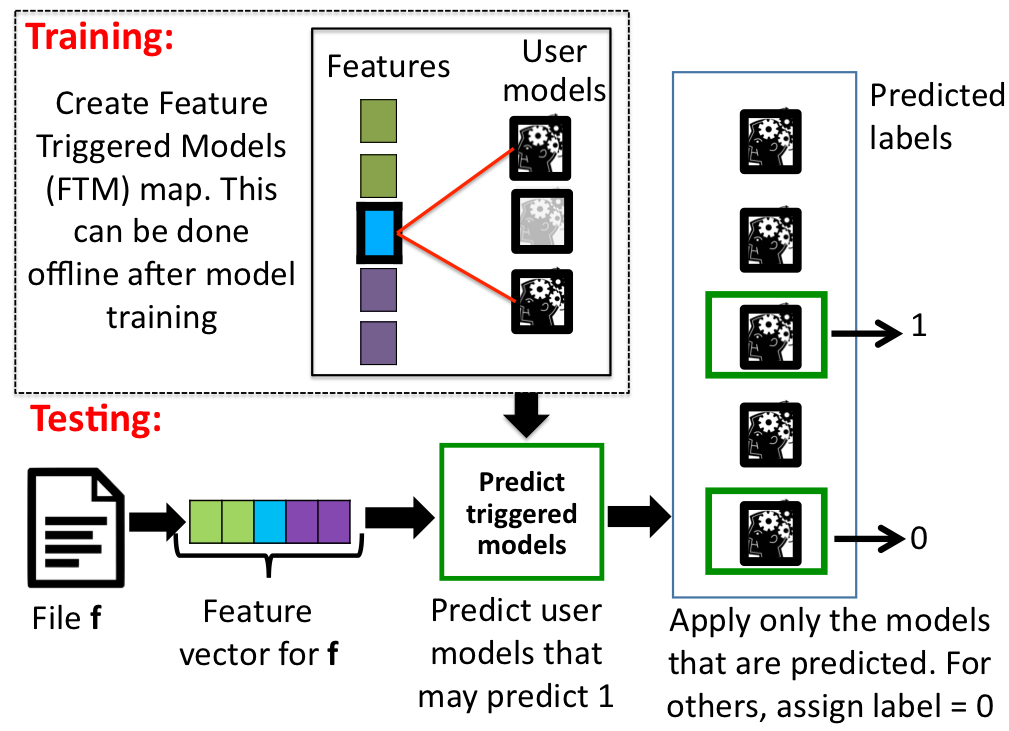
\includegraphics[width=0.7\linewidth]{FileAccess/figs/framework_withspeedup.png}
\caption{In the AFMS approach, first a Feature Triggered Models (FTM)
  map is created in an offline manner. For each test file $f$, the
  triggered models are predicted by using FTM map and only those
  models are applied on $f$. }
\label{fig:speedupframework}
\end{figure}
Figure~\ref{fig:speedupframework} shows the overall AFMS
approach. After training personalized user models, a Feature Triggered
Models (FTM) map is created to capture the user models that are \textit{triggered} by each feature. A user model $M$ is said to be \textit{triggered} by a feature $f_j$ if the feature weight for $f_j$ i.e., $w_{j,M}$ is greater than $\tau$ where $\tau \ge 0 $ is called the \textit{triggering threshold}. The value of $\tau$ determines how selective the AFMS approach is, as detailed later in this section. The FTM map needs to be
updated only when the models are re-trained. Let $N_{Meta}$ represent the number of metadata features, and let $N_{CF} = N_{Meta} + \mid\!\!U\!\!\mid$ be the number of features used in CF  models. Algorithm~\ref{alg:speedupTraining}
shows how FTM map or FTM can be obtained based on trained models. FTMs created 
using metadata models or CF models are referred to as
Metadata-FTM or CF-FTM
respectively. 

During testing of file
$f$, the \textit{triggered models} for $f$ are the set of models that
are selected to be applied on $f$ and are predicted based on the created FTM
and on the active features in $f$, i.e., the features having a non-zero for $f$. 
Algorithms~\ref{alg:speedupMetaTesting} shows how the created Metadata-FTM can be used to
obtain Triggered metadata models for test
files. For AFMS with CF models, in order to select CF models using CF-FTM, the metadata models also need to be selected using the Metadata-FTM. While using the CF-FTM, we define the active features of a file $f$ to be the non-zero metadata features of $f$ as well as the positive
predicted labels by the Triggered metadata models for $f$. This is detailed in Algorithm~\ref{alg:speedupCFTesting}. 

\begin{algorithm}[t!]
 {\fontsize{8pt}{1em}\selectfont
 \caption{Constructing FTM map}
 \label{alg:speedupTraining} 
\textbf{Input:}  
Triggering threshold: $\tau$, Trained user models (linear SVM): $M_i$ $\forall i \in [1,\mid\!\!U\!\!\mid]$ 
where $M_i$ is denoted by model parameters:  \{$w_{j,i}$\} $ \forall~j \in [0, N ]$.   \\
For Metadata-FTM, $N=N_{Meta}$ and $M_i$ represent metadata models \\ 
For CF-FTM, $N=N_{CF}$ and $M_i$ represent CF models \\ 
\textbf{Procedure: } \\
Define FTM as a hashmap mapping feature to set of models (triggered models) \\
%Initialize FTM as empty hash map\\ 
%For $i$ = 1 to $\mid\!\!U\!\!\mid$ \\ 
For each feature ($j$): \\ 
\hspace*{2mm} FTM($j$) = \{$M_i$\} s.t. $w_{j,i} \ge \tau$ \\ 
%For each user model (i.e., $M_i$) in the share \\
%\hspace*{2mm} Triggering Features = \{j : $w_{j,i} > \tau$\} \\ 
%\hspace*{2mm} For each $feat$ in Triggering Features \\ 
%\hspace*{5mm} Add user model $M_i$ as a triggered model in FTM for key = $feat$ \\ 
\textbf{Output:} FTM 
 }
 \end{algorithm}

 \begin{algorithm}[t!]
 {\fontsize{8pt}{1em}\selectfont
 \caption{Using FTM map to select metadata models} 
 \label{alg:speedupMetaTesting} 
 \textbf{Input:} 
Metadata-FTM, Test file $f$ denoted by its feature values: \{$f_j$\} $\forall j \in [1,N_{Meta}]$ \\ 
\textbf{Procedure: } 
Initialize Triggered metadata models for $f$ as empty set \\ 
Let AF($f$) := active features of $f$. AF($f$) = \{$j$\} s.t. $f_j  > 0$ \\
For each $feat$ in AF($f$): \\ 
\hspace*{2mm} Triggered metadata models for $f$ = \big\{Triggered metadata models for $f$ \\  \hspace*{45mm} $\bigcup$  Metadata-FTM($feat$) \big\} \\ 
%\hspace*{2mm} Add models in Metadata-FTM($feat$) to Triggered metadata models \\ 
\textbf{Output:} Triggered metadata models for $f$ 
 }
 \end{algorithm}

 \begin{algorithm}[t!]
 {\fontsize{8pt}{1em}\selectfont
 \caption{Using FTM map to select CF models} 
 \label{alg:speedupCFTesting} 
 \textbf{Input:} 
CF-FTM, Test file $f$  denoted by its feature values: \{$f_j$\} $\forall j \in [1,N_{CF}]$, Triggered metadata models for $f$ \\ 
\textbf{Procedure: } 
Initialize Triggered CF models for $f$ as empty set \\ 
Apply Triggered metadata models for $f$ to get predicted labels for $f$ represented by $L_{meta, f, i} \forall i \in [1, \mid\!\!U\!\!\mid] $ \\
Let AF($f$) := active features of $f$ \\ 
AF($f$) = \big\{\{$j$\} s.t. $f_j  > 0$  \, $\bigcup$  \{$N+i$\} s.t. $L_{meta, f, i} > 0 $ \big\} \\ 
For each $feat$ in AF($f$): \\ 
\hspace*{2mm} Triggered CF models for $f$ = \big\{Triggered CF models for $f$ \\  \hspace*{45mm} $\bigcup$  CF-FTM($feat$) \big\} \\ 
%\hspace*{2mm} Add models in CF-FTM($feat$) to Triggered CF models \\ 
\textbf{Output:} Triggered CF models for $f$ 
 }
 \end{algorithm}
%\vspace{-0.2in}

For $\tau=0$, the proposed AFMS approach is expected to achieve the same predictive correctness in terms of precision, recall and F-score as without AFMS, i.e., by applying every user model on each test file. When a model $M_i$ is not applied on a test file $f$, we assign its default label 0 and its confidence score to be a random negative value. 
%The test files for which a user model say $M_i$ is not applied is assigned the default label 0 and a constant value for  the confidence score. 
As a result, the ranking of the test files in terms of the prediction confidence score as per $M_i$ might be different in AFMS approach as compared to without AFMS. Since the relative ranking of test files is useful for measuring recall at 75\% precision, it is possible that AR@75P for AFMS with $\tau=0$ might differ from AR@75P without AFMS. As $\tau$ is increased, an equal or less number of models would be applied on each test file and thus the computation required per file is expected to decrease. Since less models are applied on test files, more predicted labels by the models would default to 0 and the recall is expected to degrade. By varying $\tau$, we can thus trade off the model correctness for reduction in testing computation. 
In scenarios where the available computational resources are insufficient to process the edited files, $\tau$ could be increased to process the edited files in the available resources, albeit with some loss in the predictive correctness. 
In Section~\ref{sec:exptspeedup} shows that AFMS enables a very convenient trade-off by providing significant reduction in the testing computation for marginal loss in correctness. 
Furthermore, this can also enable adaptive approaches that vary $\tau$ based on the variable rate of file edits so that more test files can be processed per unit time. 

\subsection{Complexity analysis} 
\label{sec:speedupcomplexity} 
%If for each test file, every user model in a share is applied, the average case and worst case time complexity of testing a file are both equal to $O(\mid~U~\mid)$. 
Through AFMS, the worst case testing time complexity of our system remains at $O(\mid\!\!U\!\!\mid \times R_{edit})$ since it is possible that all models in a share may be applied on the test files. However, the average case testing time complexity is $O($\textit{average number of models triggered per file}$ \times R_{edit})$. The latter may be significantly lower than the testing complexity of our system without AFMS, i.e.,  $O(\mid\!\!U\!\!\mid \times R_{edit})$. For example, it is empirically observed that for $\tau =0.5$, on average only 3.2 metadata models and 1.7 CF models are applied on test files out of 30 evaluation models. Thus on average, the testing computational requirement of our system reduces by around 9 and 18 times respectively for $\tau=0.5$. The next section provides detailed performance results for our system with AFMS. 
%Table~\ref{sec:testspeedup} shows that each feature triggers few user models and since each file has sparse features, the average number of models triggered per file can be substantially less than $\mid~U~\mid$, leading to significant testing speed-up. 
}

\comment{
\subsection{AFMS Evaluation}
\label{sec:exptspeedup}
We measure the reduction in the testing computational requirement of a file $f$ using \textit{speed-up} defined as follows: 
\begin{equation}
\label{eq:speedupgain} 
\mbox{speed-up} = \frac{\mbox{\# models applied on $f$ without AFMS}}{\mbox{\# models applied on $f$ with AFMS}}.
\end{equation}
%\CV{speedup seemed more attention grabbing than complexity. Let me know if this fits well }
\vspace{-0.2in}
\begin{figure*}
\begin{minipage}{.49\textwidth}
\epsfig{width=\linewidth,figure=FileAccess/figs/gains_thresh.eps}
\vspace{-0.15in}
\captionof{figure}{Variation of average speed-up gain with $\tau$ for metadata models}
\label{fig:gainvsThreshMeta}
\end{minipage}
\begin{minipage}{.49\textwidth}
\epsfig{width=\linewidth,figure=FileAccess/figs/gains_with_threshCF.eps}
\vspace{-0.15in}
\captionof{figure}{Variation of average speed-up gain with $\tau$ for CF models} 
\label{fig:gainvsThreshCF}
\end{minipage}
\vspace{-0.15in}
\end{figure*}

Figures~\ref{fig:gainvsThreshMeta} and \ref{fig:gainvsThreshCF} show how the speed-up varies with $\tau$ for different shares for Metadata and CF models respectively. In addition, Figures~\ref{fig:precisionvsThreshMeta} through \ref{fig:r75pvsThreshMeta} show how the precision, recall, F-score, and Recall@75\%Precision vary with $\tau$ for metadata models on different shares. The numbers provided are averaged across evaluation users and across all training and testing periods. 
%Figure~\ref{fig:gainvsThreshMeta} shows the variation of the Speed-up averaged across all test files, evaluation users and training and testing periods. 
As expected, AFMS with $\tau=0$ leads to the same F-score as without AFMS. Despite the same predictive correctness, AFMS speeds up the testing per file by 4 times on average across all shares, and by as high as 15 times for Share A. 
%(Share A). 
For $\tau=0.5$, the average speed-up across the evaluation shares is around 62 times, and is 147 times for Share A. For the same $\tau$, average F-score drops from 47\% to 43\%, average recall drops from 47\% to 37\% and average precision drops from 35\% to 34\%. Confirming to the discussion in Section~\ref{sec:AFMSdetails}, a higher $\tau$ leads to most loss in recall. 

Figures~\ref{fig:precisionvsThreshCF} through \ref{fig:r75pvsThreshCF} show the variation of the model performance metrics with $\tau$ for CF models. 
For our experiments, we have chosen the value of $\tau$ to be the same for Metadata-FTM and CF-FTM. %Also, for the calculation of speed-up for CF models as per Eq.~\ref{eq:speedupgain}, the metadata and the CF models have been considered equivalent. 
For CF models, $\tau=0$ leads to average speed-up of more than 6 times and $\tau=0.5$ leads to average speed-up of 170 times. The speed-up observed for Share A for $\tau=0.5$ is 280 times. The observed testing speed-up demonstrates that the proposed AFMS approach can significantly reduce the testing computational requirement of the proposed file recommendation system. 
\vspace{-0.2in}
% Metadata models 
\begin{figure*}[htb!]
\begin{minipage}{.49\textwidth}
\epsfig{width=\linewidth,figure=FileAccess/figs/precisions_thresh.eps}
\vspace{-0.15in}
\captionof{figure}{Variation of the average precision (AP) with $\tau$ for metadata models}
\label{fig:precisionvsThreshMeta}
\end{minipage}
\begin{minipage}{.49\textwidth}
\epsfig{width=\linewidth,figure=FileAccess/figs/recalls_thresh.eps}
\vspace{-0.15in}
\captionof{figure}{Variation of the average recall (AR) with $\tau$ for metadata models} 
\label{fig:recallvsThreshMeta}
\end{minipage}
\begin{minipage}{.49\textwidth}
\epsfig{width=\linewidth,figure=FileAccess/figs/fscore_thresh.eps}
\vspace{-0.15in}
\captionof{figure}{Variation of the average F-score (AF) with $\tau$ for metadata models}
\label{fig:fscorevsThreshMeta}
\end{minipage}
\begin{minipage}{.49\textwidth}
\epsfig{width=\linewidth,figure=FileAccess/figs/r75p_thresh.eps}
\vspace{-0.15in}
\captionof{figure}{Variation of the average recall at 75\% P (AR@75P) with $\tau$ for metadata models} 
\label{fig:r75pvsThreshMeta}
\end{minipage}
\vspace{-0.4in}
\end{figure*}

\comment{
\begin{figure}[!htb]
\epsfig{width=0.45\linewidth,figure=FileAccess/figs/gains_thresh.eps}
\vspace{-0.1in}
\caption{Variation of average speed-up gain with $\tau$ for metadata models}
\label{fig:gainvsThreshMeta}
\vspace{-0.15in}
\end{figure}
}
\begin{figure}[!htb]
\centering
\epsfig{width=0.45\linewidth,figure=FileAccess/figs/gains_vs_fscore.eps}
\vspace{-0.1in}
\caption{Variation of average speed-up gain with AF for metadata models \CV{is this figure needed?}} 
\label{fig:gainvsfscoreMeta}
\end{figure}

% CF models variations with threshold: 
\begin{figure*}[htb!]
\begin{minipage}{.49\textwidth}
\epsfig{width=\linewidth,figure=FileAccess/figs/precision_with_threshCF.eps}
\vspace{-0.1in}
\captionof{figure}{Variation of average precision (AP) with $\tau$ for CF models}
\label{fig:precisionvsThreshCF}
\end{minipage} 
\begin{minipage}{.49\textwidth}
\epsfig{width=\linewidth,figure=FileAccess/figs/recalls_with_threshCF.eps}
\vspace{-0.1in}
\captionof{figure}{Variation of average recall (AR) with $\tau$ for CF models} 
\label{fig:recallvsThreshCF}
\end{minipage} 
\begin{minipage}{.49\textwidth}
\epsfig{width=\linewidth,figure=FileAccess/figs/fscores_with_threshCF.eps}
\vspace{-0.1in}
\captionof{figure}{Variation of average F-score (AF) with $\tau$ for CF models}
\label{fig:fscorevsThreshCF}
\end{minipage} 
\begin{minipage}{.49\textwidth}
\epsfig{width=\linewidth,figure=FileAccess/figs/r75p_with_threshCF.eps}
\vspace{-0.1in}
\captionof{figure}{Variation of average recall at 75\% precision (AR@75P) with $\tau$ for CF models} 
\label{fig:r75pvsThreshCF}
\end{minipage} 
\end{figure*}

\comment{
\begin{figure}
\epsfig{width=0.95\linewidth,figure=FileAccess/figs/gains_with_threshCF.eps}
\caption{Variation of average speed-up gain with $\tau$ for CF models}
\label{fig:gainvsThreshCF}
\end{figure} 
}
\begin{figure}
\centering
\epsfig{width=0.45\linewidth,figure=FileAccess/figs/gains_vs_fscoresCF.eps}
\vspace{-0.15in}
\caption{Variation of average speed-up gain with AF for CF models. \CV{is this figure needed?}} 
\label{fig:gainvsfscoreCF}
\end{figure}


\comment{
\vspace{-0.2in}
\section{Experimental validation of AFMS }
\label{sec:exptspeedup}
We measure the reduction in the testing computational requirement of a file $f$ using \textit{speed-up} defined as follows: 
\begin{equation}
\label{eq:speedupgain} 
\mbox{speed-up} = \frac{\mbox{\# models applied on $f$ without AFMS}}{\mbox{\# models applied on $f$ with AFMS}}.
\end{equation}
%\CV{speedup seemed more attention grabbing than complexity. Let me know if this fits well }
\vspace{-0.2in}
\begin{figure*}
\begin{minipage}{.49\textwidth}
\epsfig{width=\linewidth,figure=FileAccess/figs/gains_thresh.eps}
\vspace{-0.15in}
\captionof{figure}{Variation of average speed-up gain with $\tau$ for metadata models}
\label{fig:gainvsThreshMeta}
\end{minipage}
\begin{minipage}{.49\textwidth}
\epsfig{width=\linewidth,figure=FileAccess/figs/gains_with_threshCF.eps}
\vspace{-0.15in}
\captionof{figure}{Variation of average speed-up gain with $\tau$ for CF models} 
\label{fig:gainvsThreshCF}
\end{minipage}
\vspace{-0.15in}
\end{figure*}

Figures~\ref{fig:gainvsThreshMeta} and \ref{fig:gainvsThreshCF} show how the speed-up varies with $\tau$ for different shares for Metadata and CF models respectively. In addition, Figures~\ref{fig:precisionvsThreshMeta} through \ref{fig:r75pvsThreshMeta} show how the precision, recall, F-score, and Recall@75\%Precision vary with $\tau$ for metadata models on different shares. The numbers provided are averaged across evaluation users and across all training and testing periods. 
%Figure~\ref{fig:gainvsThreshMeta} shows the variation of the speed-up averaged across all test files, evaluation users and training and testing periods. 
As expected, AFMS with $\tau=0$ leads to the same F-score as without AFMS. Despite the same predictive correctness, AFMS speeds up the testing per file by 4 times on average across all shares, and by as high as 15 times for Share A. 
%(Share A). 
For $\tau=0.5$, the average speed-up across the evaluation shares is around 62 times, and is 147 times for Share A. For the same $\tau$, average F-score drops from 47\% to 43\%, average recall drops from 47\% to 37\% and average precision drops from 35\% to 34\%. Confirming to the discussion in Section~\ref{sec:AFMSdetails}, a higher $\tau$ leads to most loss in recall. 

Figures~\ref{fig:precisionvsThreshCF} through \ref{fig:r75pvsThreshCF} show the variation of the model performance metrics with $\tau$ for CF models. 
For our experiments, we have chosen the value of $\tau$ to be the same for Metadata-FTM and CF-FTM. %Also, for the calculation of speed-up for CF models as per Eq.~\ref{eq:speedupgain}, the metadata and the CF models have been considered equivalent. 
For CF models, $\tau=0$ leads to average speed-up of more than 6 times and $\tau=0.5$ leads to average speed-up of 170 times. The speed-up observed for Share A for $\tau=0.5$ is 280 times. The observed testing speed-up demonstrates that the proposed AFMS approach can significantly reduce the testing computational requirement of the proposed file recommendation system. 
\vspace{-0.2in}
% Metadata models 
\begin{figure*}[htb!]
\begin{minipage}{.49\textwidth}
\epsfig{width=\linewidth,figure=FileAccess/figs/precisions_thresh.eps}
\vspace{-0.15in}
\captionof{figure}{Variation of the average precision (AP) with $\tau$ for metadata models}
\label{fig:precisionvsThreshMeta}
\end{minipage}
\begin{minipage}{.49\textwidth}
\epsfig{width=\linewidth,figure=FileAccess/figs/recalls_thresh.eps}
\vspace{-0.15in}
\captionof{figure}{Variation of the average recall (AR) with $\tau$ for metadata models} 
\label{fig:recallvsThreshMeta}
\end{minipage}
\begin{minipage}{.49\textwidth}
\epsfig{width=\linewidth,figure=FileAccess/figs/fscore_thresh.eps}
\vspace{-0.15in}
\captionof{figure}{Variation of the average F-score (AF) with $\tau$ for metadata models}
\label{fig:fscorevsThreshMeta}
\end{minipage}
\begin{minipage}{.49\textwidth}
\epsfig{width=\linewidth,figure=FileAccess/figs/r75p_thresh.eps}
\vspace{-0.15in}
\captionof{figure}{Variation of the average recall at 75\% P (AR@75P) with $\tau$ for metadata models} 
\label{fig:r75pvsThreshMeta}
\end{minipage}
\vspace{-0.4in}
\end{figure*}

\comment{
\begin{figure}[!htb]
\epsfig{width=0.45\linewidth,figure=FileAccess/figs/gains_thresh.eps}
\vspace{-0.1in}
\caption{Variation of average speed-up gain with $\tau$ for metadata models}
\label{fig:gainvsThreshMeta}
\vspace{-0.15in}
\end{figure}
}
\begin{figure}[!htb]
\centering
\epsfig{width=0.45\linewidth,figure=FileAccess/figs/gains_vs_fscore.eps}
\vspace{-0.1in}
\caption{Variation of average speed-up gain with AF for metadata models \CV{is this figure needed?}} 
\label{fig:gainvsfscoreMeta}
\end{figure}

% CF models variations with threshold: 
\begin{figure*}[htb!]
\begin{minipage}{.49\textwidth}
\epsfig{width=\linewidth,figure=FileAccess/figs/precision_with_threshCF.eps}
\vspace{-0.1in}
\captionof{figure}{Variation of average precision (AP) with $\tau$ for CF models}
\label{fig:precisionvsThreshCF}
\end{minipage} 
\begin{minipage}{.49\textwidth}
\epsfig{width=\linewidth,figure=FileAccess/figs/recalls_with_threshCF.eps}
\vspace{-0.1in}
\captionof{figure}{Variation of average recall (AR) with $\tau$ for CF models} 
\label{fig:recallvsThreshCF}
\end{minipage} 
\begin{minipage}{.49\textwidth}
\epsfig{width=\linewidth,figure=FileAccess/figs/fscores_with_threshCF.eps}
\vspace{-0.1in}
\captionof{figure}{Variation of average F-score (AF) with $\tau$ for CF models}
\label{fig:fscorevsThreshCF}
\end{minipage} 
\begin{minipage}{.49\textwidth}
\epsfig{width=\linewidth,figure=FileAccess/figs/r75p_with_threshCF.eps}
\vspace{-0.1in}
\captionof{figure}{Variation of average recall at 75\% precision (AR@75P) with $\tau$ for CF models} 
\label{fig:r75pvsThreshCF}
\end{minipage} 
\end{figure*}

\comment{
\begin{figure}
\epsfig{width=0.95\linewidth,figure=FileAccess/figs/gains_with_threshCF.eps}
\caption{Variation of average speed-up gain with $\tau$ for CF models}
\label{fig:gainvsThreshCF}
\end{figure} 
}
\begin{figure}
\centering
\epsfig{width=0.45\linewidth,figure=FileAccess/figs/gains_vs_fscoresCF.eps}
\vspace{-0.15in}
\caption{Variation of average speed-up gain with AF for CF models. \CV{is this figure needed?}} 
\label{fig:gainvsfscoreCF}
\end{figure}
}
}
 
%\section{Deployment }
\label{sec:deployment} 

 
\section{Related Work}
\label{sec:relatedwork}
%%
Several previous approaches have addressed the topic of file access
prediction, but with the goal of improving the I/O performance of
storage systems~\cite{Amer02fileaccess, Xia08farmer, kroeger01-usenix,
  yeh02-hpcs, yeh01-mascots, yeh01-ispass, Whittle03usingmultiple,
  Paris-stochastic}.  They aim at reducing the widening gap between
CPU and disk storage performance by prefetching files to the cache
memory.
%%
%%  FIXME: The below examples are not serving any purpose.
%%
\comment {
For instance, Amer et al.\cite{Amer02fileaccess} proposes
predictors that can reduce the number of predictions made in order to
increase the likelihood of making correct
predictions. \cite{Xia08farmer} proposes a model to infer file
correlations to optimize performance of peta-scale storage systems
while \cite{Whittle03usingmultiple} proposes a composite file access
predictor that uses multiple heuristics to predict likely successors
of files.
}
%%
%%
%%
There are a couple of key differences between our approach and the
previous ones.  Such approaches focused on modeling accesses
patterns that are generated by automated activities, whereas our focus
is on activities that are manually initiated by physical users.  This
allows us to consider certain features that could be prohibitively
expensive for caching applications.  None of the previous approaches
make predictions for completely new content.  On the other hand, by
leveraging innovative features derived from metadata and user
collaborations, our approach can make fairly good predictions for new
content.  In fact, our goal is to be able to discover useful new
content, which could be present in new or modified files.

The approach from Song et al.\cite{song14-tis} is closest to ours in
terms of providing recommendations to knowledge workers.  This
approach infers abstract tasks and frequently used workflow patterns
from historical user activity.  It then makes recommendations based on
the workflows that match current activities of the user.  Although
this approach extends beyond simple file matching, it cannot make
predictions for new content.

In terms of features, our approach is significantly different from any
of the previous approaches.  Our features are derived from rich file
metadata, including file name, path, extension, and file system
hierarchy.  These features allow our system to compare new file
activities to the learned activities in the past in terms of
similarity in the metadata attributes.  More importantly, our system
leverages metadata features to automatically generate features for
collaborative filtering in an interesting way so as to address the
cold start problem (i.e., inability to provide recommendation for new
content).  In that respect, our approach is better than the
traditional collaborative filtering approaches~\cite{linden2003amazon,
  breese1998empirical} because they suffer from the cold-start
problem.

Lastly, advanced machine learning models, e.g., factorization
machines~\cite{rendle2010factorization}, topic
models~\cite{nagori11-etncc, Ovsjanikov_topicmodeling}, and deep
neural networks~\cite{salakhutdinov2007restricted,hinton2006fast},
could be used to model access patterns. However, these techniques are
complementary and can be applied to make our system more effective.
Nonetheless, we demonstrate that simple linear SVM model can be
effectively used to build a practical system.  Most importantly, it
allows us to develop the optimization technique AFMS for significantly
reducing the classification time and improving the scalability of our
system.  This technique, in addition to the basic modeling approach,
constitutes a novel contribution of our research.

\comment{
%%% COMMENTED -- OLD CONTENT. 
% removed Ellard03attribute-basedprediction (it predicts only
% read/write pattern for newly created files

Prior works on modeling file access patterns have been mostly focused
on performance enhancement of storage systems, e.g., reducing I/O
latency by prefetching~\cite{Amer02fileaccess, Xia08farmer,
  kroeger01-usenix, yeh02-hpcs, yeh01-mascots, yeh01-ispass,
  Whittle03usingmultiple, Paris-stochastic}.  These systems make
predictions for only existing files, whereas our approach can make
predictions for newly created files too.  However, our focus is on
recommendation rather than caching.
%%  file caching don't do NLP, tokenization, etc.

The approach by Song et al.~\cite{song14-tis} is closer to our work
since it aims at assisting knowledge workers by recommending files and
actions.  It uses a data mining technique to first group similar files
into abstract tasks, and then mines frequent sequences of abstract
tasks into workflows. It then makes recommendations by identifying the
workflow that best matches the current file usage pattern of the
user. While the technique attempts to generalize beyond exact file
matching, it cannot provide recommendations for new files. In
contrast, we train personalized machine learning models that provide
recommendations even for new files. For evaluation of our approach, we
use only those test files that are new with respect to the
training files.
%As mentioned in Section~\ref{sec:introduction}, assisting knowledge workers to discover new content is essential especially given the high rate of new content generation~\cite{IDCDataGrowth}.
The ability to recommend new content is important in order to connect
knowledge workers with new data which is being generated at a
tremendous rate~\cite{IDCDataGrowth}.

Unlike all the previous works, we use much richer file metadata
including filename, path, file system hierarchy, extensions and
collaborative filtering in our models. As a result of this, our work
can also supplement existing Data Governance systems with predictive
capabilities. While our approach is not ideal for file caching in
performance sensitive applications, it could be effective in cloud
services to reduce network latency by caching files on client-facing
web servers or directly on clients.  It could also be useful for
scenarios with intermittent connectivity, such as choosing files to
cache on mobile devices.
%In contrast, our metadata features are broader, capturing not only file similarity but also hierarchical folder structure that adds to the quality of our classification model.
%% FIXME: add a referencd here..

The personalized model based file recommendation as proposed in our
paper is a content-based recommendation system. As compared to
traditional collaborative filtering based recommender
systems~\cite{linden2003amazon, breese1998empirical}, our approach
does not suffer from cold start problem, i.e., inability to recommend
a new item (file). It should however be noted that unlike traditional
collaborative filtering techniques, we do not use actual access
information. Rather, we predict the access likelihood of a user for a
particular test item and combine it with metadata features. This
enables us to circumvent the cold start problem, and thus benefit from
collaborative filtering.

Finally, advanced machine learning models such as factorization
machines~\cite{rendle2010factorization}, deep neural
networks~\cite{salakhutdinov2007restricted,hinton2006fast} and topic
models~\cite{nagori11-etncc, Ovsjanikov_topicmodeling} can also be
employed for modeling file access predictions.
%are often used in recommendation systems.  
To a large extent, these techniques are complimentary and can
contribute in making our models more effective.  Notwithstanding, we
approach the problem as a classification problem and show reasonable
effectiveness even with a simple Linear SVM-based model.  Our focus is
more on the domain specific application, with the goal of extracting
meaningful features from file metadata and user activities.

%% Several works have addressed the topic of file access prediction with
%% a goal of improving the I/O performance of storage
%% systems~\cite{Amer02fileaccess, Xia08farmer, kroeger01-usenix,
%%   yeh02-hpcs, yeh01-mascots, yeh01-ispass, Whittle03usingmultiple,
%%   Paris-stochastic}. These works attempt to reduce the widening gap
%% between CPU and disk storage performance by prefetching files to
%% cache. For instance, \cite{Amer02fileaccess} proposes predictors that
%% can reduce the number of predictions made in order to increase the
%% likelihood of making correct predictions. \cite{Xia08farmer} proposes
%% a model to infer file correlations to optimize performance of
%% peta-scale storage systems while \cite{Whittle03usingmultiple}
%% proposes a composite file access predictor that uses multiple
%% heuristics to predict likely successors of files.  While these works
%% address a relevant problem to ours, there are three key differences
%% with our work. These works focus on modeling regular file accesses
%% patterns that are primarily made by computer programs. In comparison,
%% our work is concerned with file access predictions for user activity
%% that is not from computer programs. The second key difference is that
%% the above works do not have the ability to make predictions for
%% content that is completely new while our work overcomes this shortcoming by constructing and
%% utilizing generalizable models that capture access patterns in terms
%% of metadata and collaboration based features. In fact, given the high rate of content generation in enterprises, our system is focused on new files and our evaluation framework is designed such that the test data is comprised of files that are new with respect to training. 
%% Lastly, our work is focused on recommendation applications
%% and not caching.

%% \cite{song14-tis} is closer to our work since it focuses on assisting
%% knowledge workers by recommending relevant content and
%% actions. \cite{song14-tis} infers abstract tasks and frequently used
%% workflow patterns from historical user activity. Recommendations to
%% users are made based on the workflows that their activities correlate
%% with. The approach proposed in \cite{song14-tis} is more generalizable
%% than simple file matching and can handle differently ordered
%% elements. Their approach, however, can not be extended to recommend
%% new content. Given the tremendous rate of data
%% generation~\cite{IDCDataGrowth} and of file edits\footnote{as noted in
%%   Section~\ref{sec:scalability}}, our work constructs personalized
%% models that are generalizable and can recommend, and help knowledge
%% workers discover, content that is completely new.

%% Unlike previous systems, we utilize features constructed
%% based on rich file metadata including file name, path, extensions,
%% user collaboration, file system hierarchy and folder information. As a
%% result, our system can also be used to assign likelihoods to user activities
%% based on how similar they are to the \textit{expected} activities. Our
%% work can thus complement Data Governance systems by providing
%% predictive capabilities.

%% The system proposed in this paper is primarily a \textit{content based
%%   recommendation system} which is supplemented by features based on
%% user collaboration. Compared to our modeling approach, traditional
%% approaches for Collaborative Filtering~\cite{linden2003amazon,
%%   breese1998empirical} suffer from the cold-start problem, i.e., inability
%% to provide recommendations for new
%% content. Section~\ref{sec:CFdetails} discusses how our system avoids
%% the cold start problem and can still leverage user collaboration
%% to improve its predictions.

%% Lastly, advanced machine learning models for example factorization
%% machines~\cite{rendle2010factorization}, topic
%% models~\cite{nagori11-etncc, Ovsjanikov_topicmodeling} and deep neural
%% networks~\cite{salakhutdinov2007restricted,hinton2006fast} have been
%% developed that could be used to model access patterns. These
%% techniques are complementary to our work and could be used to make the
%% proposed system more effective and efficient. Using a simple linear SVM to
%% model access patterns, we have demonstrated that it is feasible to recommend new content by using metadata
%% and collaboration based features. We have also proposed a novel approach that can potentially be extended to other content based recommender systems to significantly reduce their testing computational requirement by selecting the models to be applied on each test instance. 
%% Our work can be extended in several
%% directions, as discussed next.  \comment{
%% %%% COMMENTED -- OLD CONTENT. 
%% % removed Ellard03attribute-basedprediction (it predicts only
%% % read/write pattern for newly created files

%% Prior works on modeling file access patterns have been mostly focused
%% on performance enhancement of storage systems, e.g., reducing I/O
%% latency by prefetching~\cite{Amer02fileaccess, Xia08farmer,
%%   kroeger01-usenix, yeh02-hpcs, yeh01-mascots, yeh01-ispass,
%%   Whittle03usingmultiple, Paris-stochastic}.  These systems make
%% predictions for only existing files, whereas our approach can make
%% predictions for newly created files too.  However, our focus is on
%% recommendation rather than caching.
%% %%  file caching don't do NLP, tokenization, etc.

%% The approach by Song et al.~\cite{song14-tis} is closer to our work
%% since it aims at assisting knowledge workers by recommending files and
%% actions.  It uses a data mining technique to first group similar files
%% into abstract tasks, and then mines frequent sequences of abstract
%% tasks into workflows. It then makes recommendations by identifying the
%% workflow that best matches the current file usage pattern of the
%% user. While the technique attempts to generalize beyond exact file
%% matching, it cannot provide recommendations for new files. In
%% contrast, we train personalized machine learning models that provide
%% recommendations even for new files. For evaluation of our approach, we
%% use only those test files that are new with respect to the
%% training files.
%% %As mentioned in Section~\ref{sec:introduction}, assisting knowledge workers to discover new content is essential especially given the high rate of new content generation~\cite{IDCDataGrowth}.
%% The ability to recommend new content is important in order to connect
%% knowledge workers with new data which is being generated at a
%% tremendous rate~\cite{IDCDataGrowth}.

%% Unlike all the previous works, we use much richer file metadata
%% including filename, path, file system hierarchy, extensions and
%% collaborative filtering in our models. As a result of this, our work
%% can also supplement existing Data Governance systems with predictive
%% capabilities. While our approach is not ideal for file caching in
%% performance sensitive applications, it could be effective in cloud
%% services to reduce network latency by caching files on client-facing
%% web servers or directly on clients.  It could also be useful for
%% scenarios with intermittent connectivity, such as choosing files to
%% cache on mobile devices.
%% %In contrast, our metadata features are broader, capturing not only file similarity but also hierarchical folder structure that adds to the quality of our classification model.
%% %% FIXME: add a referencd here..

%% The personalized model based file recommendation as proposed in our
%% paper is a content-based recommendation system. As compared to
%% traditional collaborative filtering based recommender
%% systems~\cite{linden2003amazon, breese1998empirical}, our approach
%% does not suffer from cold start problem, i.e., inability to recommend
%% a new item (file). It should however be noted that unlike traditional
%% collaborative filtering techniques, we do not use actual access
%% information. Rather, we predict the access likelihood of a user for a
%% particular test item and combine it with metadata features. This
%% enables us to circumvent the cold start problem, and thus benefit from
%% collaborative filtering.

%% Finally, advanced machine learning models such as factorization
%% machines~\cite{rendle2010factorization}, deep neural
%% networks~\cite{salakhutdinov2007restricted,hinton2006fast} and topic
%% models~\cite{nagori11-etncc, Ovsjanikov_topicmodeling} can also be
%% employed for modeling file access predictions.
%% %are often used in recommendation systems.  
%% To a large extent, these techniques are complimentary and can
%% contribute in making our models more effective.  Notwithstanding, we
%% approach the problem as a classification problem and show reasonable
%% effectiveness even with a simple Linear SVM-based model.  Our focus is
%% more on the domain specific application, with the goal of extracting
%% meaningful features from file metadata and user activities.


\comment { FIXME:

Notes:
- focus on application rather than techniques

- comparison with file prefetching:  they don't predict new files

- comparison with netflix-style collaborative filtering: the dataset is
  different: no folder-like features; moreover, these techniques are
  complimentary.

- comparison with advance techniques(e.g., topic modeling) : these are complimentary techniques.

}

\comment {

Attribute-based prediction of file properties

FARMER: a novel approach to file access correlation mining and evaluation reference model for optimizing peta-scale file system performance

Design and Implementation of a Predictive File Prefetching Algorithm

Performing file prediction with a program-based successor model

Using multiple predictors to improve the accuracy of file access predictions

Using program and user information to improve file prediction performance.

Increasing predictive accuracy by prefetching multiple program and user specific files

A Program-and-User Based File Access Prediction Model

Reducing File System Latency Using a Predictive Approach

The Case for Efficient File Access Pattern Modeling

Context-Aware Prefetching at the Storage Server

File Access Prediction Using Neural Networks

File access prediction with adjustable accuracy

A stochastic approach to file access prediction

The methods of data prefetching based on user model in cloud computing

Topic Modeling for Personalized Recommendation of Volatile Items

LDA Based Integrated Document Recommendation Model for e-Learning Systems 

}
}

\section{Conclusion}
\label{sec:conclusion}

This paper presents a system to assist knowledge workers in
discovering useful new or modified content.  The system builds
personalized user models using features derived from file metadata and
user collaboration.  Our experiments showed that the basic modeling
approach does not scale well under heavy workloads. To address this
problem, we developed a novel optimization technique that improves
runtime performance without sacrificing prediction accuracy.  We also
showed how the technique can be adapted to improve the performance
significantly at marginal cost of the predictive correctness.

For future work, we could improve our system along different
directions.  Leveraging interactions observed between the features, we
could reduce dimensionality of the data for better efficiency and
effectiveness.  We could implement a weighing scheme that gives more
importance to the recent activity as it is more reflective of the
current preferences of users.  Finally, we could incorporate features
that capture producer-consumer relationship between users.

%% This paper presented a system that can assist knowledge workers to cope up with the growing enterprise data by recommending relevant new or modified content. The system trains file metadata models that can also leverage user collaboration to make more accurate predictions. 
%% %This paper presents a file recommender system that recommends relevant new or modified content to knowledge workers to assist them to cope up with the tremendous growth rate of enterprise data. The system uses file metadata and past user activity to train personalized user models and it is shown that collaboration demonstrated by the users can also be leveraged to make models more accurate. 
%% While experiments based on real enterprise activity demonstrated the feasibility of using the proposed system to recommend new content, it was observed that high testing computational requirement poses challenges for its deployment in enterprises, especially on large and active shares. In order to address this shortcoming, we proposed a novel model selection approach AFMS which is designed to leverage properties of the machine learning models used in our system, and of the enterprise data and trained models. AFMS can predict the user models to be applied on each test file and can facilitate a very convenient trade off between model correctness and testing speed. This enables implementing our system even for large and active enterprise shares using the computational resources of only a single household machine. 

%% The metadata and collaboration based features used in our system exhibit significant inter-dependence 
%% %For example knowing that the folder feature value corresponding to a folder in the file system is 1, one can conclude that the folder features corresponds to its ancenstor folders would also be 1. Such inter-dependence 
%% which could be leveraged to reduce the dimensionality of our data and improve the efficiency and efficacy of our system. In addition, during training, our system gives a uniform importance to training instances regardless of their recency. Since recent user activities are more reflective of current access patterns, weighing schemes for training instances may be investigated in future. 
%% Lastly, directed \textit{producer-consumer} relationships between users may be infered from past activity that can recommend content to a user (consumer) if it is created by other user (producer). 


%%% COMMENTED -- OLD CONTENT 
\comment{

\section{\uppercase{Future work}}
\label{sec:futurework}




The metadata features show a high degree of sparsity as is typical for
datasets of this size and scope. A file typically has very few
keywords in its path, and thus most of its token features would be
zero. Similarly, very few of its folder features, and at the maximum
of one extension feature of a file are non-zero.

While sparsity can be helpful for training user
models~{\cite{ngiam2011sparse}}, the large dimensionality of data may
negatively affect the performance of the models. It is possible that
the correctness and speed of the proposed system can be further
improved by capturing the interdependence between different features
through dimensionality reduction techniques such as Principal
Component
Analysis~\cite{jolliffe2005principal}\cite{van2009dimensionality}.
For example the folder features demonstrate substantial
interdependence and redundancy and techniques to transform them to a
suitable space may be explored.  A different approach would be to use
feature hashing \cite{FIXME} to reduce sparsity without detrimental
effects on performance.

Modeling the file metadata and user features in context of temporal
nature of file accesses could also be a potential direction for
further work. For example, giving more importance to recent events
while training user models may accommodate shifts in user interests,
leading to improved performance.  Identifying and modeling repetitive
activity may also be informative since users may be interested in
similar tasks after fixed time intervals, such as on the same day each
week.  As mentioned in Section~{\ref{sec:realdeployment}}, deployment
of the proposed system in an enterprise environment offers an online
framework to evaluate the trained models. Online model training or
update techniques can be developed that utilize the model evaluation
information to improve the trained models by adapting them to new
access patterns or newly observed features. For example, consider a
scenario where a trained model is seen to perform poorly because most
of the recent activity for a user is confined to a recently created
folder that was not part of the folder features in the trained
model. Such information can be derived from the online evaluation and
can be used to update features of the trained model and to adapt the
model to reflect the updated access patterns.\\
\indent In addition to training personalized user models, insight into
directed preferences of users may be useful for recommending
content. For example if it is determined that user $u_1$ often
accesses documents created by user $u_2$, then a recent modification
by $u_2$ may be useful information for $u_1$ and can be used as an
indicator to recommend relevant content.  \\
\indent Lastly, file access
prediction offers interesting possibilities for applications such as
information security, by offering new measures of access improbability.
}
%%% COMMENTED -- OLD CONTENT 
%%% COMMENTED -- OLD CONTENT 
\comment{
This paper presents a system that provides file recommendation to
assist knowledge workers process increasing volumes of
data.  The system utilizes natural language processing to derive
usable information from file metadata, and machine learning to train
personalized user models that have good predictive value, even for files that 
have not been observed in the past. Through extensive
experiments on real world data we demonstrate the feasibility of the
system to offer high quality recommendations, which is
reflected particularly in the significant recall at high precision
across eight shares. We also show that for shares exhibiting a high
degree of collaboration between its users, the predictions from
different user models can be combined to improve the performance of an
individual user's model.  It is observed that the trained models have
a high temporal longevity, and experience moderate performance
degradation for short training periods. Since the system
requires training personalized models for each user under
consideration, it should be applied only on shares
and users that display sufficient activity and are determined to be of
interest.
}


